%%% There are two defines: \myebookformat and \myprintformat
%%% Both false ==> PDF for online viewing or printing without binding
%%% \myprintformat == true ==> PDF for printing + binding
%%% \myebookformat == true ==> HTML for transformation into ePub

%\documentclass[a4paper,10.5pt,openright,twoside]{memoir} // for book/margins
\documentclass[a4paper,11pt,twoside]{memoir}
%\documentclass[ebook,oneside,openany]{book}%article, report
\def \myprintformat {false} % true or false
\def \myebookformat {false} % true or false

\setcounter{secnumdepth}{2}
%%% PACKAGES:

\usepackage[utf8]{inputenc}
\usepackage[english]{babel}
\usepackage{amsfonts,amsmath,amssymb,amstext,amsthm,amsbsy,amsopn}
\usepackage{mathrsfs,latexsym,stmaryrd}
\usepackage{graphicx, epsfig, wrapfig, exscale}
\usepackage{algorithm,algpseudocode}
\usepackage{lettrine}
\usepackage{natbib}
\usepackage{rotating}
\usepackage{url}
\usepackage{xspace}
\usepackage{enumerate}
\usepackage{textcomp}
\usepackage{multirow}
\usepackage{ulem}
\usepackage{ccicons}
\usepackage{tikz}
\usetikzlibrary{shapes,arrows,mindmap,trees}
\usetikzlibrary{decorations.pathmorphing}
\usetikzlibrary{decorations.markings}

\usepackage{listings}%,bera}
\definecolor{keywords}{RGB}{255,0,90}
\definecolor{comments}{RGB}{60,179,113}
\lstset{language=c++,frame=ltrb,framesep=5pt,basicstyle=\scriptsize,
  keywordstyle=\color{keywords},breaklines=true,
 commentstyle=\color{comments}emph,
 stringstyle=\ttfamily,
 %font=bera,
 showstringspaces=true}

%%% FONT:

%\usepackage{newcent}
%\usepackage{tgbonum}
%\usepackage{baskervald}
%\usepackage{DejaVuSerif}
%\usepackage[default]{droidserif}
%\usepackage{fouriernc}
%\usepackage{kmath,kerkis}

%\usepackage{palatino}
%\usepackage[sc]{mathpazo}
%\linespread{1.05}
\usepackage[T1]{fontenc}

%%% Mes commandes
\newcommand{\noi}{\noindent}
\newcommand{\II}{\mbox{\large 1\hskip -0,353em 1}}
\newcommand{\MR}{\mathcal{R}}
\newcommand{\RR} {\mbox{I \hskip -0.55 em R}}
\newcommand{\dx}{\,dx}
\newcommand{\ito}{,\dotsc,}
\newcommand{\R}{\mathbb{R}}
\newcommand{\N}{\mathbb{N}}
\newcommand{\Poly}[1]{\mathcal{P}_{#1}}
\newcommand{\abs}[1]{\left\lvert#1\right\rvert}
\newcommand{\norm}[1]{\left\lVert#1\right\rVert}
\newcommand{\pars}[1]{\left(#1\right)}
\newcommand{\bigpars}[1]{\bigl(#1\bigr)}
\newcommand{\set}[1]{\left\{#1\right\}}
\newcommand\web{\begingroup \urlstyle{tt}\Url}
\DeclareMathOperator*{\argmax}{arg\,max}
\newtheorem*{mythm}{Theorem}
\newtheorem*{mydef}{Definition}
\newtheorem*{myproof}{Proof}
\newcommand{\PP}{
\mathrm{P}
}


\ifthenelse{\equal{\myebookformat}{false}}{
% la ligne ci-dessous est à insérer obligatoirement dans le préambule du document avant \begin{document}

\usepackage[a4paper]{titre/meta-donnees}

        % les lignes en bas sont à insérer obligatoirement après \begin{document}

        %%%%%%%%%%%%%%%%%%%%%%%%%%%%%%%%%%%%%%%%%%%%%%%%%%%%%%
            %%             Commandes Meta-données               %%
            %%   à renseigner par les auteurs pour générer      %%
            %%     la couverture modèle Univ. Grenoble          %%
            %%%%%%%%%%%%%%%%%%%%%%%%%%%%%%%%%%%%%%%%%%%%%%%%%%%%%%
            %%      Fichier encodé au format ISO-8859-16        %%

            %\Sethpageshift{???mm}   %%optionnel : à décommenter si besoin pour ajout d'espace afin de center la couvérture horizontalement (valeur par défaut est -5.5mm)
            %\Setvpageshift{???mm}   %%optionnel : à décommenter si besoin pour ajout d'espace afin de center la couvérture verticalement (valeur par défaut est -15.5mm)


            %\Universite{}    %%optionnel : à décommenter et à renseigenr si vous voulez changer le non d'université
            %\Grade{}         %%optionnel : à décommenter et à renseigenr si vous voulez changer le grade
            \Specialite{Informatique}
        \Arrete{7 août 2006}
        \Auteur{Gabriel Synnaeve}
        \Directeur{Pierre Bessière}
        %\CoDirecteur{}    %%optionnel : à décommenter et à renseigenr si présence d'un Co-directeur de thèse
            \Laboratoire{Laboratoire d'Informatique de Grenoble}
        \EcoleDoctorale{École Doctorale de Mathématiques, Sciences et Technologies de l'Information, Informatique}         
        \Titre{Bayesian Programming Applied to Multi-Player Video Games}
        %\Soustitre{}      %%optionnel : à décommenter et à renseigenr si présence d'un sous-titre de thèse
            \Depot{XXX}       


        % Commande pour création de nouvelles catégories dans le jury:

            %\UGTNewJuryCategory{...NomDeLaCategorie...}{...Definition...}

        % Exemple \UGTNewJuryCategory{UGTFamille}{Membre de la famille} que nous ajoutons dans la commande \Jury ci-dessous sous la forme \UGTFamille{Jean Rousseau}{(...titre_et_affiliation...s'il_y_en_a...)}


        \Jury{
            \UGTPresident{...Civilité, Prénom et Nom...}{...titre et affiliation...}
%            \UGTPresidente{...Civilité, Prénom et Nom...}{...titre et affiliation...}

            \UGTRapporteur{...Civilité, Prénom et Nom...}{...titre et affiliation...}      %% 1er rapporteur
                \UGTRapporteur{...Civilité, Prénom et Nom...}{...titre et affiliation...}      %% second rapporteur

                \UGTExaminateur{...Civilité, Prénom et Nom...}{...titre et affiliation...}     %% 1er examinateur
                \UGTExaminateur{...Civilité, Prénom et Nom...}{...titre et affiliation...}     %% second examinateur
                \UGTExaminatrice{...Civilité, Prénom et Nom...}{...titre et affiliation...}    %% 3ème examinateur

                \UGTDirecteur{...Civilité, Prénom et Nom...}{...titre et affiliation...}       %% Directeur de thèse
%                \UGTCoDirecteur{...Civilité, Prénom et Nom...}{...titre et affiliation...}     %% Co-Directeur de thèse s'il y en a

                \UGTInvite{...Civilité, Prénom et Nom...}{...titre et affiliation...}
            \UGTInvitee{...Civilité, Prénom et Nom...}{...titre et affiliation...}
        }

%        \MakeUGthesePDG    %% très important pour générer la couvérture de thèse


}{}

%\date{}

%%% VARIABLE CONF:

\usepackage{ifthen}
\ifthenelse{\equal{\myebookformat}{true}}{
\usepackage[pagebackref]{hyperref}
\newcommand{\mapolicebackref}[1]{
    \hspace*{\fill} \mbox{\textit {\small #1}}
}
%pour gérer les backref dans la bibliographie
\renewcommand*{\backref}[1]{}
\renewcommand*{\backrefalt}[4]{%
\ifcase #1 \mapolicebackref{no citations}
    \or \mapolicebackref{cited page #2}
    \else \mapolicebackref{#1 citations pages #2}
\fi
}
  % hyperref for HTML
%\usepackage{tex4ht}
}{
\definecolor{darkblue}{HTML}{000099}
\definecolor{darkgreen}{HTML}{006600}
\definecolor{darkred}{HTML}{990000}
%\usepackage[colorlinks,citecolor=darkblue,linkcolor=darkred,urlcolor=darkgreen,pagebackref]{hyperref}
\usepackage[pdftex,
            pdfauthor={Gabriel Synnaeve},
            pdftitle={Bayesian Programming and Learning for Multi-Player Video Games: Application to RTS AI},
            pdfsubject={Ph.D thesis},
            pdfkeywords={Bayesian, machine learning, video games, artificial intelligence, RTS},
            pdfproducer={Latex with hyperref},
            pdfcreator={pdflatex},
            pagebackref]{hyperref}
\pdfinfo{
   /Author (Gabriel Synnaeve)
   /Title  (Bayesian Programming and Learning for Multi-Player Video Games: Application to RTS AI)
   %/CreationDate (D:20040502195600)
   /Subject (Ph.D thesis)
   /Keywords (Bayesian;machine learning;video games;artificial intelligence;RTS)
}
% BACKREF :
% définir un style pour les backrefs :
\newcommand{\mapolicebackref}[1]{
    \hspace*{\fill} \mbox{\textit {\small #1}}
}
%pour gérer les backref dans la bibliographie
\renewcommand*{\backref}[1]{}
\renewcommand*{\backrefalt}[4]{%
\ifcase #1 \mapolicebackref{no citations}
    \or \mapolicebackref{cited page #2}
    \else \mapolicebackref{#1 citations pages #2}
\fi
}

    % hyperref, backrefs, pdfinfo 
\ifthenelse{\equal{\myprintformat}{false}}{
\linespread{1.12}
\usepackage{fullpage}      % for electronic viewing (no headers) %%%%%%%%%%%%%%%%%%%%%%%%%%%%%%%%%%%
}{
\linespread{1.10}
\setlrmargins{*}{*}{1.14}
\checkandfixthelayout
}
}

%%% TOC:

%\usepackage[toc,page]{appendix} 
\usepackage[toc]{glossaries}
\makeglossaries
\ifthenelse{\equal{\myebookformat}{false}}{
\usepackage{minitoc}
\setlength{\mtcindent}{24pt}
\renewcommand{\mtcoffset}{0pt}
\mtcsetoffset{minitoc}{0pt}
\setlength{\mtcskipamount}{\bigskipamount}
\setcounter{minitocdepth}{1} %%% can change to 2
\renewcommand{\mtcfont}{\small\rmfamily\upshape\mdseries}
\renewcommand{\mtcSfont}{\small\rmfamily\upshape\bfseries}
\renewcommand{\mtctitle}{}
\def\chaptertoc{\minitoc \vskip 16pt}
}{}



\begin{document}

%\maketitle
\ifthenelse{\equal{\myebookformat}{false}}{
\MakeUGthesePDG
}{
\begin{center}
\begin{LARGE}Bayesian Programming and Learning for Multi-Player Video Games\end{LARGE}\\
\vspace{0.5cm}

\begin{Large}Application to RTS AI\end{Large}\\

\vspace{3cm}

\begin{large}Ph.D thesis\end{large}\\

\vspace{1cm}

\begin{Large}Gabriel Synnaeve\end{Large}\\

%\date{\today}\\

$\ccbynceu$
\end{center}
}

%%%\byncsa
\chapter*{Foreword}

\section*{Scope}
This thesis was prepared partially (2009-2010) at INRIA Grenoble, in the E-Motion team, part of the Laboratoire d'Informatique de Grenoble, and (2010-2012) at Collège de France (Paris) in the Active Perception and Exploration of Objects team, part of the Laboratoire de la Physiologie de la Perception et de l'Action. I tried to compile my research with introductory material on game AI and on Bayesian modeling so that the scope of this document can be broader than my thesis committee. The first version of this document was submitted for revision on July 20th 2012, this version contains a few changes and corrections done during fall 2012 according to the reviews of the committee. 

\section*{Remerciements}
Je tiens tout d'abord à remercier Elsa, qui m'accompagne dans la vie, et qui a relu maintes fois ce manuscrit. Je voudrais aussi remercier mes parents, pour la liberté et l'aide qu'ils m'ont apporté tout au long de ma jeunesse, ainsi que le reste de ma famille pour leur support et leurs encouragements continus. Mon directeur de thèse, Pierre Bessière, a été fabuleux, avec les bons cotés du professeur Smith : sa barbe, sa tenacité, ses histoires du siècle dernier, son champ de distorsion temporelle à proximité d'un tableau, et toujours une idée derrière la tête. Mes collègues, autant à l'INRIA qu'au Collège de France, ont été sources de discussions fort intéressantes : je les remercie tous, et plus particulièrement ceux avec qui j'ai partagé un bureau dans la (très) bonne humeur Mathias, Amaury, Jacques, Guillaume et Alex. Je tiens enfin à remercier chaleureusement tous mes amis, et en particulier ceux qui ont relus des parties de cette thèse, Étienne et Ben. 

Si c'était à refaire, je le referais surtout avec les mêmes personnes. 
% Si c'\'{e}tait \`{a} refaire, je le referais peut-\^{e}tre diff\'{e}remment mais assur\'{e}ment avec les m\^{e}mes personnes. TODO
%%% \chapter*{R\'{e}sum\'{e}}
%%% \input{abstract/resume.tex} %%% TODO
\chapter*{Abstract}
This thesis explores the use of Bayesian models in multi-player video games AI, particularly real-time strategy (RTS) games AI. Video games are in-between real world robotics and total simulations, as other players are not simulated, nor do we have control over the simulation. RTS games require having strategic (technological, economical), tactical (spatial, temporal) and reactive (units control) actions and decisions on the go. %%%This decisions, made up from incomplete/partial information, also constrains each others. As the actions of players are real-time and simultaneous, dynamic behavior adaptation is key to expert human playing.
We used Bayesian modeling as an alternative to (boolean valued) logic, able to cope with incompleteness of information and (thus) uncertainty. %%%Our claim is that, through pragmatic Bayesian modeling and machine learning, game AI programmers can achieve more adaptable and robust behaviors. %way more efficiently than by scripting (full specification of the behavior) or planning (full specification of the search problem) approaches. 
Indeed, incomplete specification of the possible behaviors in scripting, or incomplete specification of the possible states in planning/search raise the need to deal with uncertainty. Machine learning helps reducing the complexity of fully specifying such models. 
We show that Bayesian programming can integrate all kinds of sources of uncertainty (hidden state, intention, stochasticity), through the realization of a fully robotic StarCraft player. Probability distributions are a mean to convey the full extent of the information we have %%%on a problem 
and can represent by turns: constraints, partial knowledge, state space estimation and incompleteness in the model itself.

In the first part of this thesis, we review the current solutions to problems raised by multi-player game AI, by outlining the types of computational and cognitive complexities in the main gameplay types. From here, we sum up the transversal categories of problems, introducing how Bayesian modeling can deal with all of them. We then explain how to build a Bayesian program from domain knowledge and observations through a toy role-playing game example. In the second part of the thesis, we detail our application of this approach to RTS AI, and the models that we built up. For reactive behavior (micro-management), we present a real-time multi-agent decentralized controller inspired from sensory motor fusion. We then show how to perform strategic and tactical adaptation to a dynamic opponent through opponent modeling and machine learning (both supervised and unsupervised) from highly skilled players' traces. These probabilistic player-based models can be applied both to the opponent for prediction, or to ourselves for decision-making, through different inputs. Finally, we explain our StarCraft robotic player architecture and precise some technical implementation details.

Beyond models and their implementations, our contributions are threefolds: machine learning based plan recognition/opponent modeling %for symmetric players
by using the structure of the domain knowledge, multi-scale decision-making under uncertainty%for multi-scale AI, 
, and integration of Bayesian models with a real-time control program.


\clearpage

\ifthenelse{\equal{\myebookformat}{false}}{
\dominitoc
\setcounter{tocdepth}{2}
}{}
\tableofcontents
%\listoffigures
%\listoftables

\newcommand{\glos}[1]{\gls{#1}*}
\newcommand{\gloss}[1]{\glspl{#1}*}
\newcommand{\Glos}[1]{\Gls{#1}*}
\newcommand{\Gloss}[1]{\Glspl{#1}*}


\sloppy 

\chapter*{Notations}

\section*{Symbols}
\begin{tabular}{ll}
$\leftarrow$ & assignment of value to the left hand operand \\
$\sim$ & the right operand is the distribution of the left operand (random variable) \\
$\propto$ & proportionality \\
$\approx$ & approximation \\
$\#$ & cardinal of a space or dimension of a variable \\
\end{tabular}

\section*{Variables}
\begin{tabular}{ll}
$X$ and $Variable$ & random variables (or logical propositions) \\
$x$ and $value$ & values \\
$\#s = \abs{s}$ & cardinal of the set $s$ \\
$\#X = \abs{X}$ & shortcut for ``cardinal of the set of the values of $X$'' \\
$X_{1:n}$ & the set of $n$ random variables $X_1 \dots X_n$ \\
$\{x \in \Omega | Q(x)\}$ & the set of elements from $\Omega$ which verify $Q$ \\
\end{tabular}

\section*{Probabilities}

\begin{tabular}{ll}
$\PP(X) = Distribution$ & is equivalent to $X \sim Distribution$\\
$\PP(x) = \PP(X=x) = \PP([X=x])$ & Probability (distribution) that $X$ takes the value $x$ \\
$\PP(X,Y) = \PP(X\wedge Y)$ & Probability (distribution) of the conjunction of $X$ and $Y$ \\
$\PP(X|Y)$ & Probability (distribution) of $X$ knowing $Y$ \\
\end{tabular}

\section*{Conventions}
$$\PP \begin{pmatrix}X_1 \\ \vdots \\ X_k\end{pmatrix}=\PP(X) = \mathcal{N}(\mu, \sigma) \leftrightarrow \PP(X=x)= \frac{1}{(2\pi)^{k/2}\abs{\Sigma}^{1/2}}\exp(-\frac{1}{2}(x-\mu)^T\Sigma^{-1}(x-\mu))$$%,\ \mathrm{with}\ \abs{x}=k$$
$$\PP(X) = Categorical\footnote{also sometimes noted Multinomial or Histogram}(K,p) \leftrightarrow \PP(X=i) = p_i,\ \mathrm{such\ that}\ \sum_{i=1}^K p_i = 1$$

\chapter{Introduction}

\adjustmtc
\chaptertoc

\section{Contributions}

\subsection{Decentralization}

\subsection{Learnings}

\subsection{Hierarchy}

\section{Reading Map}

À la MacKay (Industry vs Research)



\chapter{Game AI}
%Babbage, Charles -- . . .every game of skill is susceptible of being played by an automaton.
%Minsky, Marvin -- It is not that the games and mathematical problems are chosen because they are clear and simple; rather it is that they give us, for the smallest initial structures, the greatest complexity, so that one can engage some really formidable situations after a relatively minimal diversion into programming. From Semantic Information Processing, p. 12. Cambridge, MA: MIT Press (1968).
% If you'd like to know, I can tell you that in your universe you move freely in three dimensions that you call space. You move in a straight line in a fourth, which you call time, and stay rooted to one place in a fifth, which is the first fundamental of probability. After that it gets a bit complicated, and there's all sort of stuff going on in dimensions thirteen to twenty-two that you really wouldn't want to know about. All you really need to know for the moment is that the universe is a lot more complicated than you might think, even if you start from a position of thinking it's pretty damn complicated in the first place. I can easily not say words like "damn" if it offends you. H2G2

%%% Some characteristics of Game AI
%%% high-level perception, commonsense reasoning, NLP, speech processing,
%%% gesture processing, planning \& counterplanning, cognitive modeling,
%%% plan recognition, soft real-time response, reactive behavior, teamwork,
%%% scheduling, path planning, spatial reasoning, temporal reasoning,
%%% opponent modeling, learning, knowledge acquisition

\begin{verse}\textit{
\\
David: What is the primary goal?\\
Joshua: You should know, Professor. You programmed me.\\
David: Oh, come on. What is the primary goal?\\
Joshua: To win the game.\\
} Wargames (1983)\end{verse}
%\lettrine[image=true, lines=3, findent=3pt, nindent=0pt]{lettrines/O.png}{r}
\lettrine{O}{r}
 is it? ``Game AI'', simultaneously a research topic, an industry standard practice, from a staple to a part of the gameplay. Its uses range from character animation, to behavior modeling and strategic play. In this chapter, we will give our educated guess about the goals of game AI, and review what exists for a broad category of games: single player games, abstract strategy games, partial information and/or stochastic games, computer games. Let us then focus on game-play (from a player point of view) characteristics of theses games so that we can enumerate game AI needs. %%% XXX
%\lettrine[image=true, lines=3, findent=3pt, nindent=0pt]{lettrines/W.png}{hat} is game AI? What are the goals of AI in games? What are its characteristics? Why is game AI an interesting subject for research? 

%%%%%%%%%%%%%%%%%%%%%%%%%%%%%%%%%%%%%%%%%%%%%%%%%%%%%%%%%%%%%%%%%% 

\section{Goals of Game AI}
%\lettrine[lines=1, lhang=.3]{W}{hat} are the goals of game AI?
Non-playing characters (NPC, also called ``mobs'') are here to stay. Being it in ever more immersive single player adventures (The Elder Scrolls V: Skyrim), part of a cooperative gameplay (World of Warcraft, Left 4 Dead) or as helpers on our side or trainers against us (``pets'', strategy games), they are of interest for the game industry, but also for robotics, to study human cognition and for artificial intelligence in the large.

\subsection{Win}
%%%Not solved: humans are the best
During the last decade, the video games industry has seen the emergence of ``e-sport''. It is the professionalization of specific competitive games at the higher levels, as in sports: with spectators, leagues, sponsors, fans and broadcasts. A %non-exhaustive 
list of major electronic sports games includes (but is not limited to): StarCraft: Brood War, Counter-Strike, Quake III, Warcraft III, Halo, StarCraft II. The first game to have had progamers was StarCraft: Brood War, in Korea, with top players earning more than top soccer players. Top players earn more than \$400,000 a year but the professional average is below, around \$50-60,000 a year \citep{TeamLiquidPGMIncome}, against the average South Korean salary at \$16,300 in 2010. Currently, Brood War is being slowly phased out to StarCraft II (still 4.9 millions players in South Korea in 2011 \citep{CitationNeeded}). There are TV channels broadcasting Brood War (OnGameNet, previously also MBC Game) or StarCraft II (GOM TV, streaming) and for which it constitutes a major chunk of the air time. %in 2010 in South Korea, the average salary for a professional StarCraft player was \$60,000 against the average salary at \$16,300\citep{StarCraftPGM}). 
``E-sport'' is important to the subject of game AI because it ensures competitiveness of the human players. It is less challenging to write a competitive AI for game played by few and without competitions than to write an AI for Chess, Go or StarCraft. E-sport, through the distribution of ``replays'' also ensures a constant and heavy flow of human player data to mine and learn from. Finally, cognitive science researchers (like the Simon Fraser University Cognitive Science Lab) study the cognitive aspects (attention, learning, re) of high level RTS playing\citep{CitationNeeded}.

Good human players, through their ability to learn and adapt, and through high-level strategic reasoning, are still undefeated. Single players are often frustrated by the NPC behaviors in non-linear (not fully scripted) games. Nowadays, video games AI could be used part of the gameplay as a challenge to the player. 
This is not the case in most of the games though, in decreasing order of resolution of the problem\footnote{We deal in gameplay potentials here, particularly considering non-linear games, current RPG and MMORPG are often linearly limited \textit{because} of the untracted``world interacting NPC'' AI problem. Otherwise, linear RPG AI fare often better than team FPS AI.}: fast FPS (first person shooters)\newglossaryentry{FPS}{name=FPS,description={First Person Shooter: egocentric shooter game, strong sub-genres are fast FPS, also called ``Quake-likes'', e.g. Quake III; and team/tactical FPS, e.g. Counter-Strike, Team Fortress 2}}, team FPS, RPG (role playing games)\newglossaryentry{RPG}{name=RPG,description={Role Playing Game, e.g. Dungeons \& Dragons based Baldur's Gate}}, MMORPG (Massively Multi-player Online RPG)\newglossaryentry{MMORPG}{name=MMORPG,description={Massively Multi-player Online Role Playing Game, distinct of RPG by the scale of cooperation sometimes needed to achieve a common goal, e.g. Dark Age of Camelot, World of Warcraft}}, RTS (Real-Time Strategy)\newglossaryentry{RTS}{name=RTS,description={Real-Time Strategy games are (mainly) allocentric economic and military simulations from an operational tactical/strategist commander viewpoint, e.g. Command \& Conquer, Age of Empires, StarCraft, Total Annihilation}}. These games in which artificial intelligences do not beat top human players on equal footing requires increasingly more cheats to even be a challenge (not for long as they mostly do not adapt). AI cheats encompass (but are not limited to):
\begin{itemize}
\item RPG NPC often have at least 10 times more hit points (health points) than their human counterparts in equal numbers,
\item FPS bots can see through walls and use perfect aiming,
\item RTS bots see through the ``fog of war'' and have free additional resources.
\end{itemize}
How do we build game robotic players (``bots'', AI, NPC) which can provide some challenge, or be helpful without being frustrating, while staying fun?


\subsection{Fun}
%%%Not solved: humans are the most fun to play with
The main purpose of gaming is entertainment. Of course, there are subgenres of serious gaming or ``gamification'' of learning, but the majority of people playing games are having fun. Cheating AI are not fun, and so the re-playability of single player games is very low. The vast majority of games which are still played after the single player mode are multi-player games, because humans are the most fun to play with. So how do we get game AI to be fun to play with? The answer seems to be 3-fold:
\begin{itemize}
\item For competitive and PvP\newglossaryentry{PvP}{name=PvP,description={Players versus Players}}
(players versus players) games: improve game AI so that it can play well \textit{on equal footing with humans},
\item for cooperative and PvE\newglossaryentry{PvE}{name=PvE,description={Players vs Environment}}
(players vs environment) games: optimize the AI for fun, ``epic wins'': the empowerment of playing your best and just barely winning,
\item give the AI all the tools to adapt the game to the players: game directors (Left 4 Dead, Dark Spore), procedural content generation (Mario PCG).
\end{itemize}
In all cases, a good AI should be able to learn for the players' actions, recognize their behavior to deal with it in the most entertaining way. Examples for a few mainstream games: World of Warcraft instances or StarCraft II missions could be less predictable (less scripted) and always ``just hard enough'', Battlefield 3 or Call of Duty opponents could have a longer life expectancy (5 seconds in some cases), Skyrim's follower NPC could avoid blocking the player in doors, or going in front when she casts fireballs.

\subsection{Programming}
How do game developers want to deal with game AI programming? We have to understand the needs of industry game AI programmers: 
\begin{itemize}
    \item computational efficiency (particularly for real-time games with advanced graphics, the AI CPU budget is low),
    \item game designers often want to remain in control of the behaviors (and editing tools have to be usable by them),
    \item scalability (as much autonomy as possible), ``debugability'' (huge states spaces due to the presence of the player(s)), re-use accross games (game independant logic).
\end{itemize}
So, programmers can ``hard code'' the behaviors and their switches, for some structuring they have finite state machines \citep{FSM_AIGameProgWisdom2003}. This solution does not scale well (exponential increase in the number of transitions), nor do they generate autonomous behavior, and they can be cumbersome for the game designers to interact with. Hierarchical FSM \citep{CitationNeeded} is a partial answer to these problems: they scale better due to the sharing of transitions between macro-states and are more readable for game designers who can zoom-in on macro/englobing states. They still represent way too much programming work for complex behavior and are not more autonomous than classic FSM. Planning (using a search heuristic in the states space) efficiently gives autonomy to virtual characters. Planners like hierarchical task networks (HTN \citep{Erol_htnplanning}, Armed Assault, Killzone 2 \citep{ArmA1_HTN,Killzone2_HTN}) or STRIPS (\citep{FikesSTRIPS}, F.E.A.R \citep{orkinGDC_FEAR}) generate complex behaviors in the space of the combinations of specified states, and the logic can be re-used accross games. The drawbacks can be a large computational budget (for many agents and/or a complex world), the difficulty to specify reactive behavior, and less (or harder) control from the game designers. Behavior trees (Halo 2 \citep{Isla}, Spore) are a popular in-between HTN and HFSM technique providing scability through a tree-like hierarchy, control through tree editing and some autonomy through a search heuristic (for valid nodes).
A transversal technique for ease of use is to program game AI with a script (LUA, Python) or domain specific language (DSL\newglossaryentry{DSL}{name=DSL,description={Domain Specific Language}}). From a programming or design point of view, it will have the drawbacks of the models it is based on. If everything is allowed (low-level inputs and outputs directly in the DSL), everything is possible at the cost of cumbersome programming, debugging and few re-use.

Even with scalable\footnote{both computationally and in the number of lines of codes to write to produce a new behavior} architectures like behavior trees or the autonomy that planning provides, there are limitations (burdens on programmers/designers or CPU/GPU):
\begin{itemize}
    \item complex worlds require either very long description of the state (in propositional logic) or high expressivity (higher order logics) to specify well-defined behaviors,
    \item the search space of possible actions increases exponentially with the interactivity (complexity) of the world, thus requiring ever more efficient pruning techniques,
    \item once human players are in the loop (ain't that the purpose of a game?), uncertainty has to be taken into account. Previous approaches can be ``patched'' to deal with uncertainty, at what cost?
\end{itemize}
Our thesis is that we can learn complex behaviors from exploration or observations (of human players) without the need to be explicitely programmed. Furthermore, the game designers can stay in control by choosing which demonstration to learn from and tuning parameters by hand if wanted. \citet{lehy04} showed it in the case of FPS AI (Unreal Tournament), with \textit{inverse programming} to learn reactive behaviors from human demonstration. We extend it to tactical and even strategic behaviors.

%%%%%%%%%%%%%%%%%%%%%%%%%%%%%%%%%%%%%%%%%%%%%%%%%%%%%%%%%%%%%%%%%% 

\section{Single Player Games}

Single player games are not the main focus of our thesis, but they present a few interesting AI characteristics. They encompass all kinds of human cognitive abilities, from reflexes to higher level thinking.

\subsection{Action games}
%%% Mario, racing, PacMan
Platform games (Mario, Sonic), time attack racing games (TrackMania), solo shoot-them-up (``schmups'', Space Invaders, DodonPachi), sports games and rhythm games (Dance Dance Revolution, Guitar Hero) are games of reflexes, skill and level knowledge. The main components of game AI in these genres is a quick path search heuristic, often with a dynamic environment. There have been Mario \citep{TogeliusMario10}, PacMan \citep{PacManCEC11} and racing competitions \citep{CarRacingWCCI08}. The winners often use (clever) heuristics coupled with a search algorithm (A* for instance). As there are no human opponents, reinforcement learning and genetic programming works well too.

XXX

\subsection{Puzzles}
%%% Myst, Tetris, point and clicks, Patience
Point and click (Monkey Island, Kyrandia, Day of the Tentacle), graphic adventure (Myst, Heavy Rain), (tile) puzzles (Minesweeper, Tetris) games are games of logical thinking and puzzle solving. The main components of game AI in these genres is an inference engine with sufficient domain knowledge (an ontology). AI research is not particularly active in the genre of puzzle games, perhaps because solving them has more to do with writing down the ontology than with using new AI techniques. A classic well-studied logic-based, combinatorial puzzle is Sudoku, which has been formulated as a SAT-solving \citep{lynce2006sudoku} and constraint satisfaction problem \citep{Simonis2005}.

%%%%%%%%%%%%%%%%%%%%%%%%%%%%%%%%%%%%%%%%%%%%%%%%%%%%%%%%%%%%%%%%%% 

\section{Abstract Strategy Games}
%%% http://en.wikipedia.org/wiki/Game_complexity
%%% http://en.wikipedia.org/wiki/Solved_board_games
\subsection{Tic-tac-toe, Minimax}
Tic-tac-toe (noughts and crosses) is a solved game\newglossaryentry{solvedgame}{name={solved game},description={a game whose outcome can be correctly predicted from any position when each side plays optimally}}, meaning that it can be played optimally from each possible position. How did it came to get solved? Each and every possible positions (26,830) have been analyzed by a Minimax (or its variant Negamax) algorithm. Minimax is an algorithm which can be used to determine the optimal score a player can get for a move in a zero-sum game\newglossaryentry{zerosumgame}{name={zero-sum game},description={a game in which the total score of each players, from one player's point-of-view, for every possible strategies, adds up to zero; \textit{i.e.} ``a player benefits only at the expense of others''}}. The Minimax theorem states:
\begin{mythm}
For every two-person, zero-sum game with finitely many strategies, there exists a value V and a mixed strategy for each player, such that (a) Given player 2's strategy, the best payoff possible for player 1 is V, and (b) Given player 1's strategy, the best payoff possible for player 2 is -V.
\end{mythm}
Applying this theorem to Tic-tac-toe, we can say that winning is +1 point for the player and losing is -1, while draw is 0. The exhaustive search algorithm which takes this property into account in described in Algorithm~\ref{alg:minimax}. The result of applying this algorithm to the Tic-tac-toe situation of Fig.~\ref{fig:TTT} is exhaustively represented in Fig.~\ref{fig:minimaxTTT}. For zero-sum games (``strictly competitive games'' as abstract strategy games discussed here), there is a (simpler) Minimax variant called Negamax, shown in Algorithm~\ref{alg:negamax} in Appendix~\ref{apdx:gameAI}.
\begin{algorithm}
\caption{Minimax algorithm}
\label{alg:minimax}
\begin{algorithmic}
\Function{mini}{depth}
    \If{$depth \leq 0$}
        \State \Return $-value()$
    \EndIf
    \State $min \gets +\infty$
    \ForAll{possible moves}
        \State $score \gets maxi(depth-1)$
        \If{$score < min$}
            \State $min \gets score$
        \EndIf 
    \EndFor
    \State \Return $min$
\EndFunction

\Function{maxi}{depth}
    \If{$depth \leq 0$}
        \State \Return $value()$
    \EndIf
    \State $max \gets -\infty$
    \ForAll{possible moves}
        \State $score \gets mini(depth-1)$
        \If{$score > min$}
            \State $max \gets score$
        \EndIf
    \EndFor 
    \State \Return $max$
\EndFunction
\end{algorithmic}
\end{algorithm}

\begin{figure}
\begin{center}
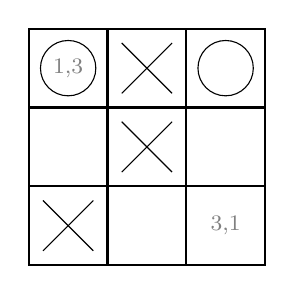
\begin{tikzpicture}
[thick]
  \foreach \x in {1,2,3}
    \foreach \y in {1,2,3}
    {
      \draw (\x,\y) +(-.5,-.5) rectangle ++(.5,.5);
    }

  \draw (1,3) node{\begin{footnotesize}\textcolor{black!50}{1,3}\end{footnotesize}};
  \draw (3,1) node{\begin{footnotesize}\textcolor{black!50}{3,1}\end{footnotesize}};

  \draw (2,3) node{\tikz \draw (-.32,-.32) -- (.32,.32);};
  \draw (2,3) node{\tikz \draw (-.32,.32) -- (.32,-.32);};

  \draw (2,2) node{\tikz \draw (-.32,-.32) -- (.32,.32);};
  \draw (2,2) node{\tikz \draw (-.32,.32) -- (.32,-.32);};

  \draw (1,1) node{\tikz \draw (-.32,-.32) -- (.32,.32);};
  \draw (1,1) node{\tikz \draw (-.32,.32) -- (.32,-.32);};

  \draw (1,3) node{\tikz \draw (0,0) circle (10pt);};

  \draw (3,3) node{\tikz \draw (0,0) circle (10pt);};
\end{tikzpicture}
\caption{A Tic-tac-toe board position, ``circles'' turn to play. The couples of numbers explain the numbering (left to right, bottom to top, starting at 1) of the grid.}
\label{fig:TTT}
\end{center}
\end{figure}

\begin{figure}
%%%\hspace{-0.8cm}
\begin{center}
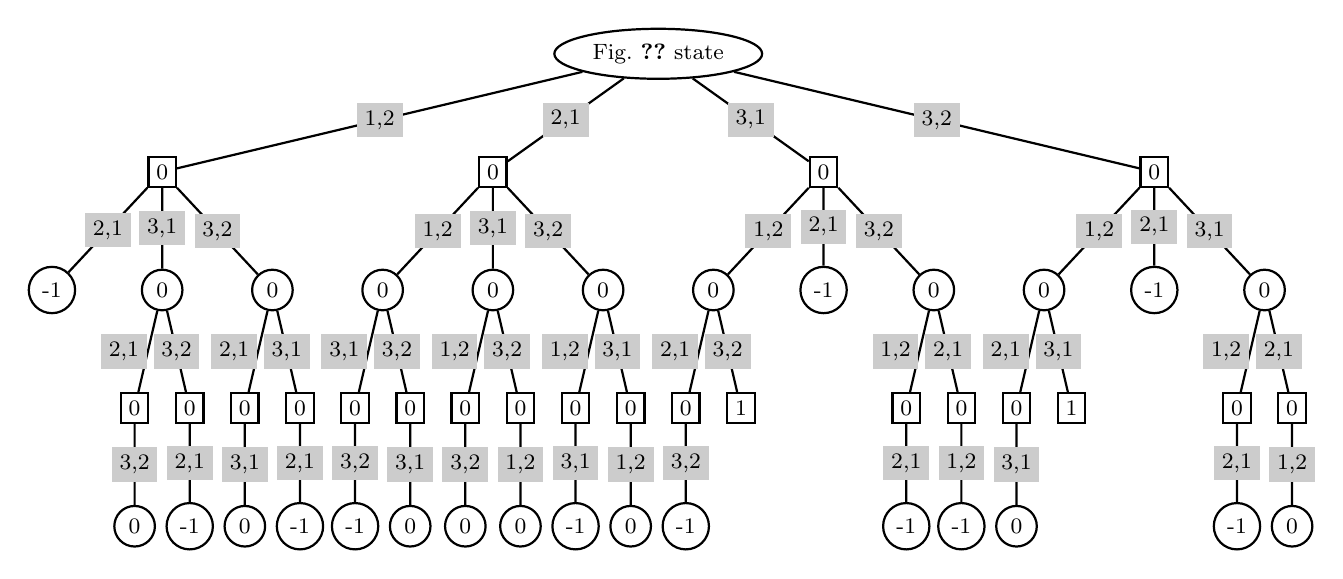
\begin{tikzpicture}
    [thick,
level 1/.style={sibling distance=42mm},
level 2/.style={sibling distance=14mm},
level 3/.style={sibling distance=7mm}
]
\begin{footnotesize}
  \node[ellipse,draw] {Fig.~\ref{fig:TTT} state}
    child {node[rectangle,draw] {0}
      child {node[circle,draw] {-1}
          edge from parent node[pos=0.5,fill=black!20] {2,1}
        }
      child {node[circle,draw] {0}
          child {node[rectangle,draw] {0}
              child {node[circle,draw] {0}
                edge from parent node[pos=0.5,fill=black!20] {3,2}}
              edge from parent node[pos=0.5,left,fill=black!20] {2,1}
            }
          child {node[rectangle,draw] {0}
              child {node[circle,draw] {-1}
                edge from parent node[pos=0.5,fill=black!20] {2,1}}
              edge from parent node[pos=0.5,fill=black!20] {3,2}
            }
          edge from parent node[pos=0.5,fill=black!20] {3,1}
        }
      child {node[circle,draw] {0}
          child {node[rectangle,draw] {0}
              child {node[circle,draw] {0}
                edge from parent node[pos=0.5,fill=black!20] {3,1}}
              edge from parent node[pos=0.5,left,fill=black!20] {2,1}
            }
          child {node[rectangle,draw] {0}
              child {node[circle,draw] {-1}
                edge from parent node[pos=0.5,fill=black!20] {2,1}}
              edge from parent node[pos=0.5,fill=black!20] {3,1}
            }
          edge from parent node[pos=0.5,fill=black!20] {3,2}
        }
      edge from parent node[pos=0.5,fill=black!20] {1,2}
    }
    child {node[rectangle,draw] {0}
      child {node[circle,draw] {0}
          child {node[rectangle,draw] {0}
              child {node[circle,draw] {-1}
                edge from parent node[pos=0.5,fill=black!20] {3,2}}
              edge from parent node[pos=0.5,left,fill=black!20] {3,1}
            }
          child {node[rectangle,draw] {0}
              child {node[circle,draw] {0}
                edge from parent node[pos=0.5,fill=black!20] {3,1}}
              edge from parent node[pos=0.5,fill=black!20] {3,2}
            }
          edge from parent node[pos=0.5,fill=black!20] {1,2}
        }
      child {node[circle,draw] {0}
          child {node[rectangle,draw] {0}
              child {node[circle,draw] {0}
                edge from parent node[pos=0.5,fill=black!20] {3,2}}
              edge from parent node[pos=0.5,left,fill=black!20] {1,2}
            }
          child {node[rectangle,draw] {0}
              child {node[circle,draw] {0}
                edge from parent node[pos=0.5,fill=black!20] {1,2}}
              edge from parent node[pos=0.5,fill=black!20] {3,2}
            }
          edge from parent node[pos=0.5,fill=black!20] {3,1}
        }
      child {node[circle,draw] {0}
          child {node[rectangle,draw] {0}
              child {node[circle,draw] {-1}
                edge from parent node[pos=0.5,fill=black!20] {3,1}}
              edge from parent node[pos=0.5,left,fill=black!20] {1,2}
            }
          child {node[rectangle,draw] {0}
              child {node[circle,draw] {0}
                edge from parent node[pos=0.5,fill=black!20] {1,2}}
              edge from parent node[pos=0.5,fill=black!20] {3,1}
            }
          edge from parent node[pos=0.5,fill=black!20] {3,2}
        }
      edge from parent node[pos=0.5,fill=black!20] {2,1}
    }
    child {node[rectangle,draw] {0}
      child {node[circle,draw] {0}
          child {node[rectangle,draw] {0}
              child {node[circle,draw] {-1}
                edge from parent node[pos=0.5,fill=black!20] {3,2}}
              edge from parent node[pos=0.5,left,fill=black!20] {2,1}
            }
          child {node[rectangle,draw] {1}
              edge from parent node[pos=0.5,fill=black!20] {3,2}
            }
          edge from parent node[pos=0.5,fill=black!20] {1,2}
        }
      child {node[circle,draw] {-1}
          edge from parent node[pos=0.5,fill=black!20] {2,1}
        }
      child {node[circle,draw] {0}
          child {node[rectangle,draw] {0}
              child {node[circle,draw] {-1}
                edge from parent node[pos=0.5,fill=black!20] {2,1}}
              edge from parent node[pos=0.5,left,fill=black!20] {1,2}
            }
          child {node[rectangle,draw] {0}
              child {node[circle,draw] {-1}
                edge from parent node[pos=0.5,fill=black!20] {1,2}}
              edge from parent node[pos=0.5,fill=black!20] {2,1}
            }
          edge from parent node[pos=0.5,fill=black!20] {3,2}
        }
      edge from parent node[pos=0.5,fill=black!20] {3,1}
    }
    child {node[rectangle,draw] {0}
      child {node[circle,draw] {0}
          child {node[rectangle,draw] {0}
              child {node[circle,draw] {0}
                edge from parent node[pos=0.5,fill=black!20] {3,1}}
              edge from parent node[pos=0.5,left,fill=black!20] {2,1}
            }
          child {node[rectangle,draw] {1}
              edge from parent node[pos=0.5,fill=black!20] {3,1}
            }
          edge from parent node[pos=0.5,fill=black!20] {1,2}
        }
      child {node[circle,draw] {-1}
          edge from parent node[pos=0.5,fill=black!20] {2,1}
        }
      child {node[circle,draw] {0}
          child {node[rectangle,draw] {0}
              child {node[circle,draw] {-1}
                edge from parent node[pos=0.5,fill=black!20] {2,1}}
              edge from parent node[pos=0.5,left,fill=black!20] {1,2}
            }
          child {node[rectangle,draw] {0}
              child {node[circle,draw] {0}
                edge from parent node[pos=0.5,fill=black!20] {1,2}}
              edge from parent node[pos=0.5,fill=black!20] {2,1}
            }
          edge from parent node[pos=0.5,fill=black!20] {3,1}
        }
      edge from parent node[pos=0.5,fill=black!20] {3,2}
    };
\end{footnotesize}
\end{tikzpicture}
\end{center}
\caption{Minimax tree with initial position at Fig.~\ref{fig:TTT} state, \textbf{nodes} are states and \textbf{edges} are transitions, labeled with the move. Leafs are end-game states: 1 point for the win and -1 for the loss. Player is ``circles'' and plays first (first edges are player's moves).}
\label{fig:minimaxTTT}
\end{figure}
\subsection{Checkers, Alpha-beta}
Checkers, Chess and Go are also zero sum, perfect-information\newglossaryentry{perfectinformationgame}{name={perfect-information game},description={a game in which all the players have complete knowledge of the (board) state of the game}}, partisan\newglossaryentry{partisangame}{name={partisan game},description={a game which is not impartial, in which a player can do actions another can not do (move a faction while the other player(s) cannot)}}, deterministic strategy game. Technically, they all can be solved by exhaustive Minimax. In practice though, it is often intractable: their bounded versions are at least in \textsc{pspace} and their unbounded versions are \textsc{exptime}-hard \citep{GPC}. The state space complexity of Checkers is the smallest of the 3 above-mentioned games with $\approxeq 5.10^20$ possible positions, and as a matter of fact, Checkers have been solved completely\citep{SchaefferBBKMLLS07}. We can see the complexity of Minimax as $O(b^d)$ with $b$ the average branching factor of the tree (to search) and $d$ the average length (depth) of the game. For Checkers $b \approxeq 10$, while the mean game length is 70 \citep{allis1994}. It is already too large to have been solved by Minimax alone (on current hardware). From 1989 to 2007, there were artificial intelligences competitions on Checkers, all using at least alpha-beta pruning: a technique to make efficient cuts in the Minimax search tree while not losing optimality.

Alpha-beta pruning (see Algorithm~\ref{alg:alphabeta}) is a branch-and-bound algorithm which (if the best nodes are searched first) can reduce Minimax to a $O(b^{d/2})=O(\sqrt{b^d})$ complexity ($O(b^{3d/4})$ for a random ordering of nodes). $\alpha$ is the maximum score than we (the maximizing player) are assured to get given what we already evaluated, while $\beta$ is the minimum score than the minimizing player is assured to get. When evaluating more and more nodes, we can only get a better estimate and so $\alpha$ can only increase while $\beta$ can only decrease. %If we find a node for us with an expected value below $\alpha$, we do not have to consider its subtree because it's sub-optimal play. If we find an expected value above $\beta$, it's sub-optimal play for the opponent. 
\begin{algorithm}
\caption{Alpha-beta algorithm}
\label{alg:alphabeta}
\begin{algorithmic}
\Function{alphabeta}{node,depth,$\alpha$,$\beta$,player}
    \If{$depth \leq 0$}
        \State \Return $value(player)$
    \EndIf
    \If{$player == us$}
        \ForAll{possible moves}
            \State $\alpha \gets \max{(\alpha, alphabeta(child,depth-1,\alpha,\beta,opponent))}$
            \If{$\beta \leq \alpha$}
                \State \textbf{break}
            \EndIf
        \EndFor
        \State \Return $\alpha$
    \Else
        \ForAll{possible moves}
            \State $\beta \gets \min{(\beta, alphabeta(child,depth-1,\alpha,\beta,us))}$
            \If{$\beta \leq \alpha$}
                \State \textbf{break}
            \EndIf
        \EndFor
        \State \Return $\beta$
    \EndIf
\EndFunction
\end{algorithmic}
\end{algorithm}
If we find a node for which $\beta$ becomes less than $\alpha$, it means that this position results from sub-optimal play. When it is because of an update of $\beta$, the sub-optimal play is on the side of the maximizing player (his $\alpha$ is not high enough to be optimal and/or the minimizing player has a winning move faster in the current sub-tree) and this situation is called an $\alpha$ cut-off. On the contrary, when the cut results from an update of $\alpha$, it is called a $\beta$ cut-off and means that the minimizing player would have to play sub-optimally to get into this sub-tree. When Starting the game, $\alpha$ is initialized to $-\infty$ and $\beta$ to $+\infty$. A worked example is given on Figure~\ref{fig:alphabeta}.
\tikzset{
alphacut/.style={postaction={decorate},
        decoration={markings,mark=at position .50 with {\draw (0.05,-.28)--(0.05,.28);\draw (-.05,-.28)--(-.05,.28);\node[right]{$\ \ \alpha \ cut$};}}},
betacut/.style={postaction={decorate},
        decoration={markings,mark=at position .50 with {\draw (0.05,-.28)--(0.05,.28);\draw (-.05,-.28)--(-.05,.28);\node[right]{$\ \ \beta \ cut$};}}},
}
\begin{figure}
%%%\hspace{-0.8cm}
\begin{center}
\begin{tikzpicture}
    [thick,
level 1/.style={sibling distance=32mm},
level 2/.style={sibling distance=14mm},
level 3/.style={sibling distance=7mm}
]
\begin{small}
  \node[circle,draw] (top) {3}
    child {node[rectangle,draw] (a) {3}
        child {node[circle,draw] (d3) {3}
            child {node[rectangle,draw] (d4) {2}}
            child {node[rectangle,draw] {3}}
        }
        child {node[circle,draw] (A) {}
            child {node[rectangle,draw] {5}}
            child {node[rectangle,draw] {} edge from parent[betacut]}
        }
    }
    child {node[rectangle,draw] (b) {0}
        child {node[circle,draw] {0}
            child {node[rectangle,draw] {0}}
        }
        child {node[circle,draw] (B) {}
            child {node[rectangle,draw] {}}
            child {node[rectangle,draw] {}}
            edge from parent[alphacut]
        }
    }
    child {node[rectangle,draw] (c) {2}
        child {node[circle,draw] {2}
            child {node[rectangle,draw] {2}}
            child {node[rectangle,draw] {1}}
        }
        child {node[circle,draw] {}
            child {node[rectangle,draw] {}}
            child {node[rectangle,draw] {}}
            edge from parent[alphacut]
        }
    };
    \node [blue,left] at (top.west) (d1) {$\alpha = 3$};
    \node [blue,left] at (a.west) (d2) {$\beta = 3$};
    \node [blue,left] at (b.west) {$\beta = 0$};
    \node [blue,left] at (c.west) {$\beta = 2$};
    \node [right] at (A.east) {$A$};
    \node [right] at (b.east) {$B$};
    \node [right] at (c.east) {$C$};
    \node [left,align=flush left] at (d1.west) {\textsc{Max}\ \ \ };
    \node [left,align=flush left] at (d2.west) {\textsc{Min}\ \ \ };
    \node [left] at (d3.west) {\textsc{Max}\ \ \ };
    \node [left] at (d4.west) {\textsc{Min}\ \ \ };
\end{small}
\end{tikzpicture}
\end{center}
\caption{Alpha-beta cuts on a Minimax tree, \textbf{nodes} are states and \textbf{edges} are transitions, labeled with the values of positions at the bottom (max depth). Here is the trace of the algorithm: \textbf{1.} descend leftmost first and evaluated 2 and 3, \textbf{2.} percolate max(2,3) higher up to set $\beta = 3$, \textbf{3.} $\beta$-cut in $A$ because its value is at least 5 (which is superior to $\beta=3$), \textbf{4.} Update of $\alpha=3$ at the top node, \textbf{5.} $\alpha$-cut in $B$ because it is at most 0 (which is inferior to $\alpha=3$), \textbf{6.} $\alpha$-cut in $C$ because it is at most 2, \textbf{7.} conclude the best value for the top node is 3.}
\label{fig:alphabeta}
\end{figure}
Prior to Checkers being solved (meaning that we have a database of which moves to play for all positions resulting from optimal play), or if playing against a sub-optimal opponent, Alpha-beta is going to be helpful to search much deeper than Minimax in the same allowed time. The best Checkers program (since the 90s), which is also the project which solved Checkers \citep{SchaefferBBKMLLS07}, Chinook, has openings and end-game (for lest than eight pieces of fewer) books, and for the mid-game (when there are more possible moves) relies on a deep search algorithm. So, appart for the beginning and the ending of the game, for which it plays by looking up a database, it used a search algorithm. As Minimax and Alpha-beta are depth first search heuristics, all programs which have to answer in a fixed limit of time use \textit{iterative deepening}, a technique which consists in fixing limited depth which will be considered maximal and evaluating this position. As it does not relies in winning moves at the bottom (remember, the search space is too big in $branching^{depth}$), we need moves evaluation heuristics. We then iterate on growing the maximal depth for which we consider moves, but we are at least sure to have a move to play in a short time (at least the greedy depth 1 found move).

\subsection{Chess, Heuristics}
With a branching factor of $\approxeq 35$ and an average game length of 80 moves \citep{Shannon_1950}, the average game-tree complexity of chess is $35^{80}\approxeq 3.10^{123}$. \citet{Shannon_1950} also estimated the number of possible actions (Shannon number) to be of the order of $10^{43}$. Chess AI needed a little more than just Alpha-beta to win against top human players (not that Checkers could not benefit it!), particularly on 1996 hardware (first win of a computer against a reigning world champion, Deep Blue on Garry Kasparov). Once an AI has openings and ending books (databases to look-up for classical moves), how can we search deeper during the game, or how can we evaluate better a situation? In iterative deepening Alpha-beta (or other search algorithms like Negascout or MTD-f), one needs to know the value of a move at the maximal depth. If it does not correspond to the end of the game, there is a need for a evaluation heuristic. Some may be straight forward, like the resulting value of an exchange in pieces points. But some strategies sacrifice a queen in favor of a more avantageous tactical position or a checkmate, so evaluation heuristics need to take tactical positions into account. In Deep Blue, the evaluation function had 8000 cases, with 4000 positions in the openings book, all learned from 700,000 grandmaster games \citep{DeepBlue}. Nowadays, Chess programs are better than deep blue and generally also search less positions. For instance, Pocket Fritz (HIARCS engine) beats current grandmasters while evaluating 20,000 positions per second (740 MIPS on a smartphone) against Deep Blue's (11.38 GFlops) 200 millions per second.

\subsection{Go, Monte-Carlo Tree Search}
With an estimated number of legal 19x19 Go positions of $2.081681994 * 10^170$ \cite{tromp2006}, and an average branching factor above Chess for gobans above 9x9, Go sets another limit for AI. MoGo \citep{GellyUCT, Gelly2006} introduced Upper Confidence Bounds for Trees (UCT\newglossaryentry{UCT}{name=UCT,description={Upper Confidence Bounds for Trees}}) for Monte-Carlo Tree Search (MCTS\newglossaryentry{MCTS}{name=MCTS,description={Monte-Carlo Tree Search}}) in Go AI successfully (being the best 9x9 and 13x13 Go program and the first to win against a pro on 9x9). The approach of MCTS is to randomly sample in the search tree (which is too big to be searched entirely), instead of systematically expanding the build tree as in Minimax, see Algorithm~\ref{alg:mcts}.
\begin{algorithm}
\caption{Monte-Carlo Tree Search algorithm. 
\textsc{SelectChild}$(node)$ and \textsc{Expand}$(node')$ are tree policy functions respectively on how to select the next move in situation $node$ (exploration or exploitation?) and how to expand the game tree of $node'$ (deep-first, breadth-first, heuristics?). \textsc{Evaluate}$(tree)$ may have 2 behaviors: \textbf{1.} if $tree$ is complete (terminal), it gives an evaluation according to games rules, \textbf{2.} if $tree$ is incomplete, it has to give an estimation (either through an heuristic or through \textsc{MCTS}). \textsc{BestChild} picks the action that leads to the better reward from $node$.}
\label{alg:mcts}
\begin{algorithmic}
\Function{MCTS}{$situation$}
    \State $node \gets$ \textsc{Node}$(situation)$
    \While{computational time left}
        \State $child \gets$ \textsc{SelectChild}$(node)$
        %%% \State \If{$child == terminal || max\ depth$}
        \State $tree \gets$ \textsc{Expand}$(child)$
        \State $child.value \gets$ \textsc{Evaluate}$(tree)$
        \State $node.children += child$
    \EndWhile
    \State \Return \textsc{BestChild}$(node)$
\EndFunction
\end{algorithmic}
\end{algorithm}


%%%%%%%%%%%%%%%%%%%%%%%%%%%%%%%%%%%%%%%%%%%%%%%%%%%%%%%%%%%%%%%%%% 

\section{Games with Uncertainty}
An exhaustive list of games or even of games genres is beyond the scope/range (XXX) of this thesis. %On the other hand, we will explain games for which randomness or incomplete information plays a key role with not-so-basic examples. 
All uncertainty boils down to incompleteness of information, being it the physics of the dice being thrown or the inability to measure what is happening in the opponent's brain. However,  we will speak of 2 types (sources) of uncertainty: extensional uncertainty, which is due to incompleteness in direct, measurable information, and intentional uncertainty, which is related to randomness in the game or in (the opponent's) decisions. The purest extensional uncertainty being acting without sensing while the purest intentional uncertainty would be for our acts to be the result of a perfect random generator. The uncertainty coming from the opponent's mind/cognition lies in between, depending on the simplicity to model the game as an optimization procedure. The harder the game is to model, the harder it is to model the trains of thoughts our opponents can follow.

\subsection{Monopoly}
In Monopoly, there is few hidden information (\textit{Chance} and \textit{Community Chest} cards only), but there is randomness in the throwing of dice\footnote{Note that the sum of two uniform distributions is not a uniform but a Irwin-Hall, $\forall n>1, P([\sum_{i=1}^n{(X_i\in U(0,1))}]=x) \propto \frac{1}{(n-1)!}\sum_{k=0}^n(-1)^k{n\choose k}\max{((x-k)^{n-1},0)}$, converging towards a Gaussian (central limit theorem).}, and a substantial influence of skill (player's decision). A very basic playing strategy would be to just look at the ruturn on investment (ROI) with regard to prices, rents and frequencies, choosing only based on the money you have and the possible actions of buying or not. A less naive way to play should evaluate the questions of buying with regard to what we already own, what others own, our cash and advancement in the game. The complete state space is huge (places for each players $\times$ their money $\times$ their possessions), but according to \cite{MonopolyMarkov}, we can model the game for one player (as he has no influence on the dice rolls and decisions of others) as a Markov process on 120 ordered pairs: 40 board spaces $\times$ possible number of doubles rolled so far in this turn (0, 1, 2). With this model, it is possible to compute more than simple ROI and derive applicable and interesting strategies. So, even in monopoly, which is not lottery playing or simple dice throwing, a simple probabilistic modeling yields a robust strategy. Additionally, \cite{MonopolyFrayn05} used genetic algorithms to generate the most efficient strategies for portfolio management. %We observe that the main difficulty of Monopoly: randomness in a gameplay in which we have to make up a strategy, can be dealt with with probabilistic modeling. 
Monopoly is an example of a game in which we have complete direct information about the state of the game, intentional uncertainty due to the roll of the dice (randomness) can be dealt with thanks to probabilistic modeling (Markov processes here). The opponent's actions are relatively easy to model due to the fact that the goal is to maximize cash and that there are not many different efficient strategies (not many Nash equilibrium if it were a stricter game) to attain it.

%\subsection{Diplomacy}
%\subsection{Bridge}
\subsection{Battleship}
Battleship (also called ``naval combat'') is a guessing game generally played with two 10x10 grids for each players: one is the player's ships grid, and one is to remember/infer the opponent's ships positions. The goal is to guess where the enemy ships are and sink them by firing shots (torpedoes). There is \textbf{incompleteness} of information but no randomness. Incompleteness can be dealt with with probabilistic reasoning. The classic setup of the game consist in two ships of length 3 and one ship of each lengths of 2, 4 and 5; in this setup, there are 1,925,751,392 possible arrangements for the ships. The way to take advantage of all possible information is to update the probability that there is a ship for all the squares each time we have additional information. So for the 10x10 grid we have a 10x10 matrix $O_{1:10,1:10}$ with $O_{i,j} \in \{true,false\}$ being the $i$th row and $j$th column random variable of the case being occupied. With $ships$ being unsunk ships, we always have $$\sum_{i,j}P(O_{i,j}=true) = \frac{\sum_{k\in ships}length(k)}{10 \times 10}$$. For instance for a ship of size 3 alone at the beginning we can have prior distributions on $O_{1:10,1:10}$ by looking at combinatorics of its placements (see Fig.~\ref{fig:battleship}). We can also have priors on where the opponent likes to place her ships. Then each round we will either hit or miss in $i,j$. When we hit, we know $P(O_{i,j}=true)=1.0$ and will have to revise the probabilities of surrounding areas, and everywhere if we learned the size of the ship, with possible placement of ships. If we did not sunk a ship, the probabilities of uncertain (not 0.0 or 1.0) positions around $i,j$ will be highered according to the sizes of remaining ships. If we miss, we know $P(O_{i,j})=false$ and can also revise (lower) the surrounding probabilities, an example of that effect is shown in Fig.~\ref{fig:battleship}. Battleship is a game with few intensional uncertainty (no randomness), particularly because the goal quite strongly conditions the action (sink ships as fast as possible) but a large part of extensional uncertainty (incompleteness of direct information), which goes down rather quickly once we act, if we update a probabilistic model of the map/grid.

\begin{figure}[h!]
\begin{center}
\includegraphics[width=7.8cm]{images/battleship_board_3_init_annotated.png} \includegraphics[width=7.8cm]{images/battleship_board_3_1miss.png}
\caption{Left: visualization of probabilities for squares to contain a ship of size 3 ($P(O_{i,j})=true$) initially, assuming uniform distribution of this type of ship. Annotations correspond to the \textit{number of combinations} (on six, the maximum number of conformations), Right: same probability after a miss in (5, 5). The larger the white area the higher the probability.}
\label{fig:battleship}
\end{center}
\end{figure}


\subsection{Poker}

%\section{Card Games}
\citep{gunn}

%%%%%%%%%%%%%%%%%%%%%%%%%%%%%%%%%%%%%%%%%%%%%%%%%%%%%%%%%%%%%%%%%% 

\section{FPS}
\subsection{Gameplay}
\subsection{FPS AI}
\subsubsection{Industry}
\subsubsection{Research}
\begin{itemize}
\item Quake 3 AI (industry standard w/o squad AI) \citep{waveren-02-artificial}
\item Killzone 2, F.E.A.R \citep{orkinGDC_FEAR} (planning), Crysis 2, BF3: industry standards with squad AI
\item Research:
\begin{itemize}
\item \citep{lehy04}
\item \citep{Laird01} (cognitive architecture)
\item others (\citep{Hladky_anevaluation} ANN, ...)
\item UT Challenge (c.f. CIG)
\end{itemize}
\end{itemize}
\subsubsection{Challenges}

%%%%%%%%%%%%%%%%%%%%%%%%%%%%%%%%%%%%%%%%%%%%%%%%%%%%%%%%%%%%%%%%%% 

\section{(MMO)RPG}

\subsection{Gameplay}
\subsection{RPG AI}
\subsubsection{Industry}
\subsubsection{Research}
\citep{Cutumisu09}
\subsubsection{Challenges}
\citep{SYNNAEVE:MMORPG}


%%%%%%%%%%%%%%%%%%%%%%%%%%%%%%%%%%%%%%%%%%%%%%%%%%%%%%%%%%%%%%%%%% 

\section{RTS}

\subsection{Gameplay}
XXX 

In chronological order, RTS include (but are not limited to): Ancient Art of War, Herzog Zwei, Dune II, Warcraft, Command \& Conquer, Warcraft II, Command \& Conquer: Red Alert, Total Annihilation, Age of Empires, StarCraft, Age of Empires II, Tzar, Cossacks, Homeworld, Battle Realms, Ground Control, Spring Engine: Balanced Annihilation, Warcraft III, Total War, Warhammer 40k, Sins of a Solar Empire, Supreme Commander, StarCraft II.

Both \citep{Human-LevelAIKillerApplication} and \cite{gunn} propose that RTS AI is one of the most challenging genres, because all levels in the hierarchy of decisions are of importance.

\subsection{RTS AI}
\subsubsection{Industry}
\subsubsection{Research}
\subsubsection{Challenges}

%%%%%%%%%%%%%%%%%%%%%%%%%%%%%%%%%%%%%%%%%%%%%%%%%%%%%%%%%%%%%%%%%% 

\section{Game Characteristics}

For a complementary taxonomy of video games and AI, see \cite{gunn}.
\subsection{Combinatory}
\subsection{Partial information}
%%%\subsection{Multiplayer}
%%%\subsection{PvE}
\subsection{Randomness}
\subsection{Time Constant(s)}
\subsection{Learning Curve}
\subsection{Recap}
\begin{sidewaystable}
\begin{tabular}{|l|ccccc|}
\hline 
Game & Combinatory & Vertical cont. & Horizontal cont. & Partial Info. & Randomness \\
\hline
Checkers & $b\approxeq 10; n\approxeq 70$ & none & none & no & no \\
Chess & $b\approxeq 35; n\approxeq 80$ & none & none & no & no \\
Go & $b\approxeq 250-300; n\approxeq 150-200$ & none & some & no & no \\
%Monopoly 
%Battleship
Limit Poker & $b\approxeq 3$\footnote{fold,check,raise} $;n/hour \in [20\dots240]$\footnote{number of decisions taken per hour} & some & few & much & much \\
Time Racing & & & & & \\
(TrackMania) & $b\approxeq 50-1,000$\footnote{$\{X \times Y\}$ sampling$\times$50Hz}$;n/min \approxeq 60$ & full & much & no & no \\
Team FPS & $b\approxeq 100-5,000$\footnote{\label{samplingFPS}$\{X \times Y \times Z\}$ sampling$\times$50Hz + firing} $;n/min \approxeq 100$\footnote{\label{apmFPS}60 ``continuous move actions''+ 40 (mean) fire actions per sec} & some & much & some & some \\
(Counter-Strike) & & & & & \\
(Team Fortress 2) & & & & & \\
FFPS duel & $b\approxeq 200-10,000$\footref{samplingFPS} $;n/min \approxeq 100$\footref{apmFPS} & some & much & some & ($\approxeq$)no \\
(Quake III) & & & & & \\
MMORPG & $b\approxeq 50-100$\footnote{in RPGs, the player does not have to aim and positioning plays a lesser role than in FPS} $;n/min \approxeq 60$\footnote{move and use abilities/cast spells} & much & much & few & moderate \\
(WoW, DAoC) & & & & & \\
RTS & $b\approxeq 200$\footnote{atomic dir/unit $\times$ \# units + constructions + productions}$;n/min=APM\approxeq 300$\footnote{for progamers, counting group actions as only one action}& some & some & much & no\\
(StarCraft) & & & & & \\
\hline
\end{tabular}
\end{sidewaystable}

%%%%%%%%%%%%%%%%%%%%%%%%%%%%%%%%%%%%%%%%%%%%%%%%%%%%%%%%%%%%%%%%%% 

\section{Player Characteristics}

%%% Timings, reflexes, modeling, goals, utility, backtracking, induction, ...

In all these games, knowledge and learning plays a key role. Humans compensate their lack of (conscious) computational power with pattern matching, abstract thinking and efficient memory structures. 
\subsection{Virtuosity}
Skill
\subsection{Deduction}
\subsection{Induction}
\subsection{Decision-Making}
%%%\subsection{Psychology}
\subsection{Recap}
%%% https://en.wikipedia.org/wiki/Cognition
\begin{sidewaystable}
\begin{tabular}{|l|ccccccc|}
\hline 
Game & Virtuosity & Deduction & Induction & Decision-Making & \multicolumn{3}{c|}{Knowledge} \\
     & (sensory-motor) & (analysis) & (abstraction) & (acting) & game & map & opponent \\
Checkers &   & ++ & &   & ++& &+ \\
Chess &   & ++ & &   & ++& &+ \\
Go &   & ++ & + &   & ++& &+ \\
Limit Poker &   & + & + & ++ & ++& &++ \\
Time Racing & ++ &   &   &   & +&++&  \\
(TrackMania) & & & & & & & \\
Team FPS & & & & & & & \\ 
(Counter-Strike) & & & & & & & \\ 
(Team Fortress 2) & & & & & & & \\ 
FFPS duel & ++ & + &   & + & +&++&+ \\
(Quake III) & & & & & & & \\ 
MMORPG & + & + & + & ++ & +&++&+ \\
(WoW, DAoC) & & & & & & & \\ 
RTS & ++ & ++ & ++ & ++ & ++&+&++ \\
(StarCraft) & & & & & & & \\
\hline
\end{tabular}
\end{sidewaystable}

%%%%%%%%%%%%%%%%%%%%%%%%%%%%%%%%%%%%%%%%%%%%%%%%%%%%%%%%%%%%%%%%%% 

\section{An interesting problem}
\subsection{Simulated but stochastic}
Human players (ally or foes), and sometimes (most of the time) stochasticity in the rules of the game (fog of war, randomness, etc.).

\chapter{Bayesian Modeling of Multi-player Games}
\chaptertoc

%%% Nothing in Nature is random. ... A thing appears random only through the incompleteness of our knowledge.
%%% - Benedict Spinoza -

\begin{quotation}\textit{
On voit, par cet Essai, que la théorie des probabilités n'est, au fond, que le bon sens réduit au calcul; elle fait apprécier avec exactitude ce que les esprits justes sentent par une sorte d'instinct, sans qu'ils puissent souvent s'en rendre compte.
\vspace{0.2cm} \\
One sees, from this Essay, that the theory of probabilities is basically just common sense reduced to calculus; it makes one appreciate with exactness that which accurate minds feel with a sort of instinct, often without being able to account for it.}
\begin{flushright}Pierre-Simon de Laplace (1814)\end{flushright}\end{quotation}

\lettrine{H}{ere}, we now present the use of probability theory as an alternative to logic, transforming incompleteness into uncertainty. Bayesian models can deal with both intentional and extensional uncertainty, that is: uncertainty coming from intentions of the players or the stochasticity of the game, as well as uncertainty coming from imperfect information and the model's limits. We will first show how these problems are addressed by probabilities and how to structure a full Bayesian program. We illustrate the approach with a model evaluated on a simulated \glos{MMORPG} situation.

%Bot AI has to be adaptive, robust, multi-scale.
%Why?
%\begin{itemize}
%\item The bot can't cheat (at least it's not fun!)
%\item The bot can't assume optimal play from the opponent when the problem is so large
%\item The bot can learn from others games, self past games, self current game
%\item The bot can't be in the head of your opponent (meta-)
%\end{itemize}

\section{Characteristics of Game AI}

\subsection{Partial information}
If the AI has perfect information, behaving realistically is the problem. Cheating bots are not fun, so either AI should just use information available to the players, or it should fake having only partial information. In probabilistic modeling, sensor models allow for the computation of the state $S$ from observations $O$ by asking $\PP(S|O)$. One can easily specify or learn $\PP(O|S)$: either the game designers specify it, or the bot uses perfect information to get $S$ and leanrs (counts) $\PP(O|S)$. Then infer $\PP(S|O) = \frac{\PP(O|S).\PP(S)}{\PP(O)}$ (Bayes rule). Incompleteness of information is just uncertainty about the full state.

\subsection{Randomness}
Some games have inherent stochasticity (variable random action effects) part of the gameplay, and even for other games, an AI can't assume optimal play from the opponent. In the context of state estimation and control, dealing with this randomness require ad-hoc methods for scripting of boolean logic, while it is dealt with natively with probabilistic models. Where a program would have to test for the action effect/value $V$ to be in a given interval to decide on a given course of action $A$, a probabilistic models just computes $\PP(A|E) = \frac{\PP(E|A).\PP(A)}{\PP(E)}$.

\subsection{Vertical continuity}
Abstracting higher level cognitive functions (strategy and tactics for instance) is an efficient way to break the complexity barrier of writing game AI. Exploiting the vertical continuity, i.e. the conditioning of higher level thinking on actions, is totally possible in a hierarchical Bayesian model. With strategies as values of $S$ and tactics as values of $T$, $\PP(T|S)$ gives the conditioning of $T$ on $S$ and thus enables us to evaluate only those $T$ values that are possible with given $S$ values.

\subsection{Horizontal continuity}
Real-time games may use discrete time-steps (24Hz for instance for StarCraft), it does not prevent temporal continuity in strategies, tactics and, most strongly, actions. There are several Bayesian models able to deal with sequences, filter models, from which \newglossaryentry{HMM}{name=HMM,description={Hidden Markov Model, a dynamic Bayesian network estimating hidden states following a Markov process from observations}}Hidden Markov Models (\glos{HMM}) \citep{Rabiner}, Kalman filters \citep{Kalman1960} and particle filters \citep{particleFiltering} are specializations of. With states $S$ and observations $O$, filter models under the Markov assumption represent the joint $\PP(S^0).\PP(O^0|S^0).\prod_{t=1}^T[\PP(S^t | S^{t-1}).\PP(O^t|S^t)]$.

\subsection{Autonomy and Programming}
Autonomy is the ability to deal with new states, the challenge of autonomous characters arises from state spaces too big to be fully specified (in scripts / FSM). Again, probabilistic modeling enables one to recognize unspecified states as soft mixtures of known states, of deal with unknown state as an incomplete version of a known state which subsumes it. Autonomy can also be reached through learning, being it through online or offline learning. Offline learning is used to learn parameters that does not have to be specified by the programmers and/or game designers. One can use data or experiments with known/wanted situations (supervised learning, reinforcement learning), or explore data (unsupervised learning) or game states (evolutionary algorithms). Online learning can provide adaptivity of the AI to the player and/or its own competency playing the game.

\section{The Bayesian Programming Methodology}
The reverend Thomas Bayes is the first credited to have worked on inversing probabilities: by knowing something about the probability of $A$ given $B$, how can one draw conclusions on the probability of $B$ given $A$? Bayes theorem states: $$\PP(A|B) = \frac{\PP(B|A)P(A)}{\PP(B)}$$
\cite{Laplace} rediscovered this theorem and published the work of inductive reasoning by using probabilities. Later, by extending logic to \textit{plausible reasoning}, \cite{Jaynes} arrived at the same properties than \cite{Kolmogorov33} probability theory. Plausible reasoning originates from logic, whose statements have degrees of plausibility represented by real numbers. %We note ``the conditional plausibility that A is true, given that B is true'' $A|B$.
Adding consistency: a) all the possible ways to reach a conclusion leads to the same result, b) information cannot be ignored, c) two equal states of knowledge have the same plausibilities; Jaynes derived the ``product-rule'' ($\PP(AB)=\PP(A\cap B)=\PP(A|B)\PP(B)$) and the ``sum-rule'' ($\PP(A+B)=\PP(A)+\PP(B)-\PP(AB)$ or $\PP(A\cup B) = \PP(A)+\PP(B)-\PP(A\cap B)$) of probabilities. As for rules of inferences, the links between logic and plausible reasoning are direct, with $C=[A\Rightarrow B]$:
\begin{itemize}
    \item modus ponens $$\frac{[A\Rightarrow B] \wedge [A=true]}{B=true}$$ translates to $$\PP(B|AC)=\frac{\PP(AB|C)}{\PP(A|C)}$$
    \item modus tollens $$\frac{[A\Rightarrow B] \wedge [B=false]}{A=false}$$ translates to $$\PP(A|C\neg B)=\frac{\PP(A \neg B|C)}{\PP(\neg B|C)}$$
\end{itemize}
Also, additionally to the two strong logic syllogisms above, plausible reasoning gets two weak syllogisms, from:
\begin{itemize}
    \item $$\PP(A|BC)=\PP(A|C)\frac{\PP(B|AC)}{\PP(B|C)}$$ we get $$\frac{[A\Rightarrow B] \wedge [B=true]}{A\ \mathrm{becomes\ more\ plausible}}$$
    \item $$\PP(B| C\neg A)=\PP(B|C)\frac{\PP(\neg A|BC)}{\PP(\neg A|C)}$$ we get $$\frac{[A\Rightarrow B] \wedge [A=false]}{B\ \mathrm{becomes\ less\ plausible}}$$
\end{itemize}

Indeed, this was proved by \cite{Cox46}, producing Cox's theorem (also named Cox-Jayne's theorem):
\begin{mythm}
A system for reasoning which satisfies:
\begin{itemize}
    \item divisibility and comparability, the plausibility of a statement is a real number,
    \item common sense, in presence of total information, reasoning is isomorphic to Boolean logic,
    \item consistency, two identical mental states should have the same degress of plausibility,
\end{itemize}
is isomorphic to probability theory.
\end{mythm}
So the degrees of belief,of any consistent induction mechanism, verify Kolmogorov's axioms. \cite{DeFinetti37} showed that if reasoning is made in a system which is not isomorphic to probability theory, then it is always possible to find a \textit{Dutch book} (a set of bets which guarantees a profit regardless of the outcomes).


Inspired by plausible reasoning, we present Bayesian programming, a formalism that can be used to describe entirely any kind of Bayesian model. It subsumes Bayesian networks and Bayesian maps, as it is equivalent to probabilistic factor graphs \cite{Diard03}. There are mainly two parts in a \newacronym{BP}{BP}{Bayesian program}\glos{BP}, the \textbf{description} of how to compute the joint distribution, and the \textbf{question(s)} that it will be asked. 

The description consists in exhibiting the relevant \textit{variables} $\{X^1,\dots,X^n\}$ and explain their dependencies by \textit{decomposing} the joint distribution $\PP(X^1\dots X^n | \delta, \pi)$ with existing preliminary (\textit{prior}) knowledge $\pi$ and data $\delta$. The \textit{forms} of each term of the product specify how to compute their distributions: either parametric forms (laws or probability tables, with free parameters that can be learned from data $\delta$) or recursive questions to other Bayesian programs.

Answering a question is computing the distribution $\PP(Searched | Known)$, with $Searched$ and $Known$ two disjoint subsets of the variables. 
%%%$P(Searched | Known) = \begin{small} \frac{\sum_{Free}P(Searched\ Free\ Known)}{P(Known)} \end{small} = \frac{1}{Z}\times \sum_{Free} P(Searched\ Free\ Known)$. 
\begin{eqnarray}
& & \PP(Searched | Known) \\
& = & \frac{\sum_{Free}\PP(Searched,\ Free,\ Known)}{\PP(Known)} \\
& = & \frac{1}{Z}\times \sum_{Free} \PP(Searched,\ Free,\ Known)
\end{eqnarray}

General Bayesian inference is practically intractable, but conditional independence hypotheses and constraints (stated in the description) often simplify the model. There are efficient ways to calculate the joint distribution like message passing and junction tree algorithms \citep{Pearl,Nai04,Koller}. Also, there are different well-known approximation techniques: either by sampling with Monte-Carlo (and Monte-Carlo Markov Chains) methods \citep{MacKay,Andrieu}, or by solving a simpler model which approximate the full joint as with variational Bayes \citep{Beal}.

%\begin{small}
\begin{eqnarray*}
BP
\begin{cases}
Desc.
    \begin{cases}
    Spec. (\pi)
        \begin{cases}
        Variables\\
        Decomposition\\
        Forms\ (Parametric\ or\ Program)
        \end{cases}\\
    Identification\ (based\ on\ \delta)
    \end{cases}\\
Question
\end{cases}
\end{eqnarray*}
%\end{small}


For the use of Bayesian programming in sensory-motor systems, see \citep{PRDMSMS}. For its use in cognitive modeling, see \citep{Colas10}. For its first use in video games (first person shooter gameplay, Unreal Tournament), see \citep{LeHy04}. \$\$\$


To sum-up, by viewing probabilities as an extension of logic, the method by which to build Bayesian models gets clearer: there is a strong parallel between writing a Bayesian program and logic or declarative programming. In order:
\begin{enumerate}
    \item Isolate the variables of the problem: it is the first prior that the programmer puts into the system. The variables can be anything, from existing input or output values of the problem to abstract/aggregative values or parameters of the model. Discovering which variable to use for a given problem is one of the most complicated form of machine learning.
    \item Suppose and describe the influences and dependencies between these variables. This is another prior that the programmer can have on the problem, and learning the structure between these variables is the second most complicated form of learning.
    \item Fill the priors and conditional probabilities parameters. The programmer needs to be an expert of the problem to put relevant parameters, although this is the easiest to learn from data once variables and structure are specified. Learning the structure can be seen as learning the parameters of a fully connected model (and then removing dependencies where are the less influent parameters) but most of these kinds of model are totally untractable.
\end{enumerate}
In the following, we will show this method applied to a simulated \glos{MMORPG} fight situation.


%%% How?
%%% \begin{itemize}
%%% \item Bayesian programming methodology
%%% \item When in doubt, toss the distribution to your neighbour
%%% \item Exploit gameplay/game rules structure
%%% \item Learn and eat data for breakfast
%%% \item Meta- can be solved by being (globally) stateless and applying the same model as self on the opponent with her sensory inputs
%%% \end{itemize}

\section{Modeling of a Bayesian MMORPG player}
We will now present a model of a \glos{MMORPG} player with the Bayesian programming framework \citep{SYNNAEVE:MMORPG}. A role-playing game (RPG) consist in the incarnation by the human player of an avatar with a class (warrior, wizard, rogue, priest...) having different skills, spells, items, health points, stamina/energy/mana (magic energy) points. Massively Multi-Player Online Role-Playing Games (e.g. World of Warcraft, AION, EVE Online, Star Wars: The Old Republic) consist in controlling a single character, which can earn experience, as well as equip always better items to increase its health points, damage per second and other skills (heals, enhancements...). Players are immersed in a unique and persistent (thus the ``massively multi-player'') world, with its history and epic battles. Players have to combat each others (\glos{PvP}) due to the factions they belong to. They also have to team-up and battle against the environment (\glos{PvE}) to aquire better items and level-up. This is a cooperative task in which human players fight together against different NPC. And more specifically here, we modeled the ``druid'' class, which is complex because it can cast spells to deal damages or other negative effects as well as to heal allies or enhance their capacities (``buff'' them). The model described here deals only with a sub-task of a global AI for autonomous NPC. The problem that we try to solve is: how do we choose which skill to use and on which target in a PvE battle? Possible targets are all our allies and foes. Possible skills are all that we know, we will just try and get a distribution over target and skills and pick the most probable combination that is yet possible to achieve (enough energy/mana, no cooldown). For that, we first choose what should be the target given all surrounding variables: is an ally near death that he should be healed, which foe should we focus our attacks on? Once we have the distribution over possible targets, we search the distribution about our skills, pondered by the one on targets. However, some variables can be things that humans subconsciously interpolate from perceptions.

\subsection{Variables}

A simple set of variables is as follows. We have the $n$ characters as possible targets; each of them has a lot of bound variables. Health/Hit points ($HP$) are discretized in 10 levels, from the lower to the higher. Distance ($D$) is discretized in 4 zones around the robot character: \textit{contact} where it can attack with a contact weapon, \textit{close}, \textit{far} and (\textit{very far}) to the further for which we have to move even for shooting the longest distance weapon/spell. Ally ($A$) is a Boolean variable mentioning if character $i$ is allied with the robot character. Delta hit points ($\Delta HP$) is a 3-valued interpolated value from the previous few seconds of fight that informs about the $i$th character getting wounded or healed (or nothing). Imminent death ($ID$) is also an interpolated value that encodes $HP$, $\Delta HP$ and incoming attacks/attackers. This is a Boolean variable saying if the $i$th character if going to die anytime soon. This is an example of what we consider that an experienced human player will infer automatically from the screen and notifications. Class ($C$), simplified over 4 values, gives the type of the $i$th character: a Tank can take a lot of damages and taunt enemies, a Contact damager can deal huge amounts of damage with contact weapons (rogue, barbarian...), Ranged stands for the class that deals damages from far away (hunters, mages...) and Healers are classes that can heal (in considerable amounts). The Resist variable is the combination of binary variables of resistance to certain types of (magical) damages into one variable. With 3 possible resistances we get ($2^3$) 8 possible values. For instance ``$R_i=FireNat$'' means that the $i$th character resists fire and nature-based damages. Armor (physical damages) could have been included, and the variables could have been separated. The skill variable takes here all the possible skills for the given character, and not only the available ones to cast at the moment to be able to have reusable probability tables (i.e. learnable tables).

\begin{itemize}
    \item Target: $T^{t-1,t} \in \{t_1\dots t_n\}$ at $t$ and $t-1$ (previous action). $T^t$ is also abusively noted $T$ in the rest of the model.
    \item Hit Points: $HP_1 \dots HP_n$ s.t. $HP_i \in [0\dots 9]$
    \item Distance: $D_1 \dots D_n$ s.t. $D_i \in \{Contact, Close, Far, VeryFar\}$
    \item Ally: $A_1 \dots A_n$ s.t. $A_i \in \{true, false\}$
    \item Derivative Hit Points: $\Delta HP_1 \dots \Delta HP_n$ s.t. $\Delta HP_i \in \{-, 0, +\}$
    \item Imminent Death: $ID_1 \dots ID_n$ s.t. $ID_i \in \{true, false\}$
    \item Class: $C_1 \dots C_n$ s.t. $C_i \in \{Tank, Contact, Ranged, Healer\}$
    \item Resists: $R_1 \dots R_n$ s.t. $R_i \in \{Nothing, Fire, Ice, Nature, FireIce, IceNat, FireNat, All\}$
    \item Skill: $S \in \{Skill_1 \dots Skill_m\}$
\end{itemize}

\subsection{Decomposition}

\subsubsection{Target selection}
The joint distribution is simplified (by conditional independence of variables) as:
\begin{eqnarray}
\PP(T, T^{t-1}, HP_{1:n}, D_{1:n}, A_{1:n}, \Delta HP_{1:n}, ID_{1:n}, C_{1:n}) = \\
\PP(T^{t-1}).\PP(T|T^{t-1}).\prod_{i=1}^n [ \PP(HP_i | A_i, C_i, T).\PP(D_i | A_i, t).\PP(A_i | T)\\
\PP(\Delta HP_i | A_i, C_i, T).\PP(C_i | A_i, T).\PP(ID_i | T) ]
\end{eqnarray}
We want to compute the probability distribution on the variable Target ($T$), so we have to consider the joint distribution with all variables on which Target ($T$) is conditionally dependant : the previous value of Target ($T^{t-1}$), and all the variables on each character (except for Resists). The probability of a given target depends on the previous one (it encodes the previous decision and so all previous states). The health (or hit) points ($HP_i$) depends on the facts that the $i$th character is an ally ($A_i$), on his class ($C_i$), and if he is a target ($T$). Such a conditional probability table should be learned, but we can already foresee that a targeted ally with a tanking class ($C=tank$) would have a high probability of having low hit points ($HP$) because taking it for target means that we intend to heal him. The distance of the unit $i$ ($D_i$) is more probably far if unit $i$ is an enemy ($A_i=false$) and we target it ($T=i$) as our kind of druid attacks with ranged spells and does not fare well in the middle of the battlefield. The probability of the $i$th character being an ally depends on if we target allies of foes more often: that is $\PP(A_i|T)$ encodes our propensity to target allies (with heals and enhancements) or foes (with damaging or crippling abilities). The probability that the $i$th units is being damaged (losing hit points: $\Delta HP_i=``-''$) is higher for foes ($A_i=false$) with vulnerable classes ($C_i=healer$) that are more succeptible to be targeted ($T=i$), and also for allies ($A_i=true$) whose role is to take most of the damages ($C_i=tank$). As for $A_i$, the probability of $ID_i$ is driven by our %soft evidence 
inclination of targeting characters near death. The probability of $C_i$ is driven by the distribution of foes and allies population, tuned with a soft evidence of which classes our druid human player will target more frequently. %Each and every time, if $T \neq i$, the probability of the left variable is given according to the uniform distribution. For the task of computing the distribution on Target, the joint distribution is simplified (by conditional independence of variables) as:


\subsubsection{Skill selection}
For skill selection, we need additional variables. The joint distribution of the updated model is: 
\begin{eqnarray}
\PP(S, T^{t-1,t}, HP_{1:n}, D_{1:n}, A_{1:n}, \Delta HP_{1:n}, ID_{1:n}, C_{1:n}, R_{1:n}) = \\
\PP(S).\PP(T^t|T^{t-1}).\PP(T^{t-1}).\prod_{i=1}^n [ \PP(HP_i | A_i, C_i, S, T).\PP(D_i | A_i, S, T).\PP(A_i | S, T) \\
        \PP(\Delta HP_i | A_i, S, T). \PP(R_i | C_i, S, T). \PP(C_i | A_i, S, T) ]
\end{eqnarray}
As previously for targets, we are interested in the conditional probabilities of each character's state variables given other state variables and given our target ($T$) and the skill that we use ($S$). If we target the $i$th unit ($T=i$), happening to be an allied ($A_i=true$) tank ($C_i=tank$) with a ``big heal'' ($S=big\_heal$), the probability that they will have low hit points ($HP_i=0$ or $1$ (very low)) is very high. Some skills have optimal ranges to be used at and so $\PP(D_i)$ will be affected. As we use heals $s_h\in \{heals\}$ exclusively on allies, $\PP(A_i=true|S=s_h) =1.0$. Conversely, as we use attacks ($s_a\in \{damage\}$) exclusively on foes, $\PP(A_i=false|S=s_a)=1.0$. The probability that the $i$th units is being damaged ($\Delta HP_i=``-''$) will top when we use a heal ($S=heal$) on an ally, as we want to maintain everyone alive. The one of the resist to ``nature based effects'' ($R_i=nature$) for skills involving ``nature'' damage ($s \in \{nature\_damage\}$) will be very low as it will be useless to use spells that the receiver is protected against. The probability that the $i$th character will die soon ($ID_i$) will be high if $i$ is targeted ($T=i$) with a big heal or big instant damage ($S=big\_heal$ or $S=big\_damage$, depending on whether $i$ is an ally or not). %For the task of computing the distribution on Skill we use:


\subsection{Parameters}

\begin{itemize}
    \item $\PP(T^{t-1})$ is unknown and unspecified (uniform). In the question, we always know what was the previous target, except when there was not one.
    \item $\PP(T|T^{t-1})$ is a probability corresponding to the propensity to switch targets. It can be learned, or uniform if there is no previous target (it the prior on the target then).
    \item $\PP(S)$ is unknown and so unspecified, it could be a prior.
    %\item $\PP(Left\_Value | Right\_Value)$ All others are \textit{learned tables}.
    \item $\PP(HP_i | A_i, C_i, S, T)$ is a $2\times4\times m \times 2$ probability table, indexed on if the $i$th character is an ally or not, on its class, on the skills ($\#S=m$) and on where it is the target or not. It can be learned (and/or parametrized), for instance $\PP(HP_i=x|a_i,c_i,s,t)=\frac{1+\mathrm{count}(x,a_i,c_i,s,t)}{10+\mathrm{count}(a_i,c_i,s,t)}$.
    \item $\PP(D_i | A_i, S, T)$ is a $4\times2 \times m \times 2$ (possibly learned) probability table.
    \item $\PP(A_i | S, T)$ is a $2 \times m \times 2$ (possibly learned) probability table.
    \item $\PP(\Delta HP_i | A_i, S, T)$ is a $3 \times 2 \times m \times 2$ (possibly learned) probability table.
    \item $\PP(R_i | C_i, S, T)$ is a $8 \times 4 \times m \times 2$ (possibly learned) probability table.
    \item $\PP(C_i | A_i, S, T)$ is a $4 \times 2 \times m \times 2$ (possibly learned) probability table.
\end{itemize}

\subsection{Identification}

If there were only perceived variables, learning the right conditional probability tables would just be counting and averaging. However, some variables encode combinations of perceptions and passed states. We could learn such parameters through the EM algorithm but we propose something simpler for the moment as our ``not directly observed variables'' are not complex to compute, we compute them from perceptions as the same time as we learn. For instance we map in-game values to their discrete values for each variables online and only store the resulting state ``compression''. In the following Results part however, we did not apply learning but instead manually specified the probability tables to show the effects of gamers' \textit{common sense} rules and how it/they can be correctly encoded in this model.

\subsection{Questions}

In any case, we ask our (updated) model:\\
\begin{equation}
P(S,T|t^{t-1},hp_{1:n},d_{1:n}, a_{1:n}, \Delta hp_{1:n}, id_{1:n}, c_{1:n}, r_{1:n})
\end{equation}
Which means that we want to know the distribution on $S$ and $T$ knowing all the state variables. We then choose to do the highest scoring combination of $S \wedge T$ that is available (skills may have cooldowns or cost more mana/energy that we have available).

As (Bayes rule) $P(S,T) = P(S|T).P(T)$, to decompose this question, we can ask:
$$P(T | t^{t-1}, hp_{1:n},d_{1:n}, a_{1:n}, \Delta hp_{1:n}, id_{1:n}, c_{1:n})$$ 
Which means that we want to know the distribution on $T$ knowing all the relevant state variables, followed by (with the newly computed distribution on $T$):
$$P(S | T, hp_{1:n},d_{1:n}, a_{1:n}, \Delta hp_{1:n}, id_{1:n}, c_{1:n}, r_{1:n})$$ 
in which we use this distribution on $T$ to compute the distribution on $S$ with:
$$P(S=skill_1 | \dots) = \sum_T P(S=skill_1 | T, \dots).P(T)$$
We here choose to sum over all possible values of T. Note that we did not ask:\\
$P(S|T=most\_probable , \dots)$ but computed instead
$$\sum_T P(S|T,hp_{1:n},d_{1:n}, a_{1:n}, \Delta hp_{1:n}, id_{1:n}, c_{1:n}, r_{1:n})$$
In presence of several possible targets and skills, this computation may have a high complexity, so we could choose not to do the sum and use and instantiate ``most probable values'', for instance of Target, but there we would make a choice earlier and so lose information. There are possibly good combinations of $S$ and $T$ for a value of $T$ that is not the most probable one. This downside may be so hard that we may want to reduce the complexity of computation by simplifying our model or its computation to be able to sum. We propose a solution in the discussion.


Here is the full Bayesian program corresponding to this model:

\begin{eqnarray*}
BP
\begin{cases}
Desc.
    \begin{cases}
    Spec. (\pi)
        \begin{cases}
        Variables\\
        S, T^{t-1,t}, HP_{1:n}, D_{1:n}, A_{1:n}, \Delta HP_{1:n}, ID_{1:n}, C_{1:n}, R_{1:n}\\
        Decomposition\\
        \PP(S, T^{t-1,t}, HP_{1:n}, D_{1:n}, A_{1:n}, \Delta HP_{1:n}, ID_{1:n}, C_{1:n}, R_{1:n}) = \\
        \PP(S).\PP(T|T^{t-1}).\PP(T^{t-1}).\prod_{i=1}^n [ \PP(HP_i | A_i, C_i, S, T).\PP(D_i | A_i, S, T).\PP(A_i | S, T) \\
                \PP(\Delta HP_i | A_i, S, T). \PP(R_i | C_i, S, T). \PP(C_i | A_i, S, T) ]\\
        Forms\\
        \mathrm{probability\ tables\ parametrized\ on\ wether\ }i\ \mathrm{is\ targeted}\\
        \end{cases}\\
    Identification\ (using\ \delta)\\
    \mathrm{learning\ (e.g.\ Laplace\ succession\ law)\ or\ manually\ specified}\\
    \end{cases}\\
Question\\
\PP(S,T|T^{t-1}, HP_{1:n}, D_{1:n}, A_{1:n}, \Delta HP_{1:n}, ID_{1:n}, C_{1:n}, R_{1:n})
\end{cases}
\end{eqnarray*}

\subsection{Example}

\begin{figure}[h!]
\begin{center}
\includegraphics[width=5cm]{images/wow_fight1.png} \hspace{1.5cm} \includegraphics[width=5cm]{images/wow_fight2.png}
\caption{Example setup A (left) and B (right). There are 2 foes and 2 players taking damages (``MT'' and ``tank''). Players with stars can heal allies, players with dotted lines will soon die ($ID=true$). Our model controls the blue character, green players are allies, while red characters are foes. The larger the surrounding ellipse is, the more health points the characters have.}
\label{fig:wow_fight}
\end{center}
\end{figure}

This model has been applied to a simulated situation with 2 foes and 4 allies while our robot took the part of a ``druid'', a versatile class that can cast spells to do direct damages, damages over time, buff (enhancements), debuff, crowd-control, heal and heal over time. We display a schema of this situation in Fig.~\ref{fig:wow_fight} The arrows indicate foes attacks on allies. MT stands for ``main tank'', Add for ``additional foe''. We worked with the skills corresponding to a Druid. HOT stands for heal over time, DOT for damage over time, ``abol'' for abolition and ``regen'' for regeneration, a ``buff'' is an enhancement and a ``dd'' is a direct damage. ``Root'' is a spell which disables the target to move for a short period of time, useful to flee or to put some distance between the enemy and the druid to cast attack spells. ``Small'' spells are usually faster to cast than ``big'' spells. The difference between setup A and setup B is simply to test the concurrency between healing and dealing damage and the changes in behavior if the player can lower the menace (damage dealer).

\begin{eqnarray*}
Skills \in \{ small\_heal, big\_heal, HOT, poison\_abol, malediction\_abol,\\
            buff\_armor, regen\_mana, small\_dd, big\_dd, DOT, debuff\_armor, root \}
\end{eqnarray*}

We did not do the ``Identification'' part, which consists in learning the probability tables from observations. To keep things simple and because we wanted to analyze the answers of the model, we worked with manually defined probability tables, %. So we introduced ``soft evidences'', indeed parameters that will modify the conditional probability tables, 
which we will change to watch their effects on the full behavior of the model. 
%For instance the
%``soft evidence that a selected target is foe'' and the ``soft evidence that a selected target will soon die ($ID=true$)'' that will consequently modify the probability tables of $P(A_i)$ and $P(ID_i)$ respectively. 
%probability that a selected target is a foe $\PP(A_i|T=i)$ and the probability that a selected target will soon die will $\PP(ID_i=``soon''|T=i)$
In the experiments, we will try different values for the ``soft evidence that a selected target will soon die'', that is $\PP(ID_i | T=i)$, and see how the behavior of the agent changes. 
We set the probability to target the same target as before ($\PP(T^t=i|T^{t-1}=i)$) to 0.4 and the previous target to ``Lich'' so that the prior probability for all other 6 targets is 0.1 (4 times more chances to target the Lich than any other character). 
We set the probability to target an enemy (instead of an ally) $\PP(A_i=false|T=i)$ to 0.6. This means that our robotic druid is mainly a damage dealer and just a backup healer. For the ``target selection'' sub-model, we can see on Fig.~\ref{fig:wow_target} (left) that the evolution from selecting the main foe ``Lich'' to selecting the ally ``Tank'' is driven by the increase of 
``soft evidence that a selected target will soon die'' and our robot eventually moves on targeting their ``Tank'' ally (to heal them). We can see on Fig.~\ref{fig:wow_target} (right) that, at some point, the robotic Druid prefers to kill the dying ``add'' (additional foe) to save their ally Tank instead of healing them. Note that there is no variable showing the relation between ``Add'' and ``Tank'' (the first is attacking the second, who is taking damages from the first), but this could be taken into account in a more complete model.

\begin{figure}[h!]
\begin{center}
\includegraphics[width=7.8cm]{images/wow_distrib_target1.png} \includegraphics[width=7.8cm]{images/wow_distrib_target2.png}
\caption{Left: probabilities of targets depending on the soft evidence that a target is dying ($\PP(ID_i=true | T=i)$) with setup A (no ally is risking death). Right: same, with setup B (the ``tank'' ally is risking death).}
\label{fig:wow_target}
\end{center}
\end{figure}
\begin{figure}[h!]
\begin{center}
\includegraphics[width=7.8cm]{images/wow_distrib_skill1.png} \includegraphics[width=7.8cm]{images/wow_distrib_skill2.png}
\caption{Left: Probabilities of skills depending on the soft evidence that a target is dying ($\PP(ID_i=true|T=i)$) with setup A (no ally is risking death). Right: same, with setup B (the ``tank'' ally is risking death).}
\label{fig:wow_skill}
\end{center}
\end{figure}

For the ``skill selection'' model, we can see on Fig.~\ref{fig:wow_skill} the influence of $ID_i$ on Skill which is coherent with the Target distribution: either, in setup A (left), we evolve with the increase of $\PP(ID_i=true|Target=i)$ to choose to heal our ally or, in setup B (right), to deal direct damage (and hopefully, kill) the foe attacking him. As you can see here, when we have the highest probability to attack the main enemy (``Lich'', when $\PP(ID_i=true|Target=i)$ is low), who is a $C=tank$, we get a high probability for the Skill \textit{debuff\_armor}. We only cast this skill if the debuff is not already present, so perhaps that we will cast \textit{small\_dd} instead. To conclude this example, Fig.~\ref{fig:wow_target_skill} shows the distribution on $\PP(T,S|all\_status\_variables)$ with setup A and the probability to target the previous target (set to ``Lich'' here) only $\approx 2$ times greater than any other character (so that we focus less on the same character), soft evidences $\PP(ID_i=true|Target=i)=0.9$ and $\PP(A_i=false|Target=i)=0.6$. On the decision-making side of this model, a simple approach would be a greedy one: if the first couple $(T,S)$ is already done or not available, we perform the second, and so on.


\begin{figure}[h!]
\begin{center}
\includegraphics[width=12.5cm]{images/wow_distrib_target_skill.png}
\caption{Log-probabilities of Target and Skill with setup A, and $\PP(ID_i=true|T=i)=0.9, \PP(A_i=false|T=i)=0.6$. This plot corresponds to the answer to the full question on which decision-making has to be done.}
\label{fig:wow_target_skill}
\end{center}
\end{figure}

\subsection{Discussion}
%%% 
%%% This model has to be applied in a real MMORPG, out of its simulated sandbox, to reveal all its shortcomings and be updated. We can already think of some future difficulties, for instance there is a possibility for many games that the Skill variable will be very big and that it will imply a too high computational cost. For that concern, we propose to clusterize the skills in global skills ($GS$) (as it can be seen in the description of the example). This approach to break down the complexity of computation is general and can be used with other variables. The skill variable $S$ can then be the subset of skills corresponding to the clustering of $GS$, for instance we could have:
%%% 
%%% $$GS \in \{SkillHeal, SkillBuff, SkillAttack, SkillDebuff\}$$
%%% $$S = SkillHeal \in \{skill_1 \dots skill_j\}$$
%%% $$S = SkillBuff \in \{skill_{j+1} \dots skill_k\}$$
%%% $$S = SkillAttack \in \{skill_{k+1} \dots skill_l\}$$
%%% $$S = SkillDebuff \in \{skill_{l+1} \dots skill_m\}$$
%%% 
%%% Global skills joint distribution: as for the “Skill joint distribution” without Resists. It will take advantage of splitting between allies and foes.
%%% 
%%% \begin{eqnarray*}
%%% P(GS,T,HP_{1:n},D_{1:n},A_{1:n},\Delta HP_{1:n}, ID_{1:n}, C_{1:n}) = \\
%%% P(GS).P(T).\prod_{i=1}^n [ P(HP_i | A_i, C_i, GS, T).P(D_i | A_i, GS, T).P(A_i | GS, T)\\
%%%                         .P(\Delta HP_i | A_i, GS, T).P(ID_i | GS, T).P(C_i | A_i, GS, T)]
%%% \end{eqnarray*}
%%% 
%%% Specialized skills joint distribution:
%%% 
%%% \begin{eqnarray*}
%%% P(S,GS,T,HP_{1:n},D_{1:n},A_{1:n},\Delta HP_{1:n}, ID_{1:n}, C_{1:n}, R_{1:n}) = \\
%%% P(S|GS).P(T).\prod_{i=1}^n [ P(HP_i | A_i, C_i, S, T).P(D_i | A_i, S, T).P(A_i | S, T)\\
%%%                         .P(\Delta HP_i | A_i, S, T).P(R_i | C_i, S, T).P(ID_i | S, T).P(C_i | A_i, S, T)]
%%% \end{eqnarray*}
%%% for the corresponding S. So that we can ask the question:
%%% $$P(S | GS, T, hp_{1:n}, d_{1:n}, a_{1:n}, \Delta hp_{1:n}, id_{1:n}, c_{1:n}, r_{1:n})$$
%%% 
%%% that will trigger $P(GS|T,\dots)$, itself triggering $P(T|all\_state\_variables)$. Choosing to do with or without the intermediate $GS$ computation, regrouping abilities by types, is mainly a question of computational time.

This limited model served the purpose of presenting Bayesian programming in practice. While it was used in a simulation, it showcases the approach one can take to break down the problem of autonomous control of \glos{npc}. The choice of the skill or ability to use and the target on which to use it puts hard constraints on every others decisions the autonomous agent has to take to perform its ability action. Thus, such a model shows that:
\begin{itemize}
    \item cooperative behavior is not too hard to incorporate in a decision (instead of being hard-coded),
    \item it can be learned, either from observations of a human player or by reinforcement (exploration),
    \item it is computationally tractable (for use in all games), the inference is just a series of ``probabilistic \textit{if}s'',
\end{itemize}
Moreover, using this model on another agent than the one controlled by the AI can give a prediction on what it will do, resulting in human-like, adaptive, playing style.

We did not kept at the research track of Bayesian modeling MMORPG games due to the difficulty to work on these types of games: the studios have too much to lose to ``farmer'' bots to accept any automated access to the game. Also, there are no sharing format of data (like replays) and the invariants of the game situations are fewer than in RTS games. Finally, RTS games have international AI competitions which were a good motivation to compare our approach with other game AI researchers.

\chapter{RTS AI: \textit{StarCraft: Broodwar}}
\chaptertoc

\begin{quotation}\textit{
lala}
\\
truc
\end{quotation}

\section{How does the game work}

\subsection{RTS Gameplay}
We first introduce the basic components of a real-time strategy (RTS) game. The player is usually referred as the ``commander'' and perceives the world in an allocentric ``God's view'', performing mouse and keyboard actions to give orders to units (or squads of units) within a circumvented area (the ``map''). In a RTS, players need to gather resources to build military units and defeat their opponents. To that end, they often have \textit{worker units} (or extraction structures) than can gather resources needed to build \textit{workers}, \textit{buildings}, \textit{military units} and \textit{research upgrades}. Workers are often also builders (as in StarCraft) and are weak in fights compared to military units. Resources may have different uses, for instance in StarCraft: minerals are used for everything, whereas gas is only required for advanced buildings or military units, and technology upgrades. Buildings and research upgrades define technology trees (directed acyclic graphs) and each state of a 
\newglossaryentry{techtree}{name={tech tree},description={abbreviation for ``technological tree'', state of the technology (buildings, researches, upgrades) which are unlocked/available to a given player.}}
%\newglossaryentry{techtree}{name={tech tree},description={abbr. for ``technological tree'', the state of buildings and technologies evolution (technologies which are unlocked) of a given player}}
\glos{techtree} (or \newglossaryentry{buildtree}{name={build tree},description={abbrev. for ``buildings tree'', state of the buildings (and thus production) unlocked by a player}}\glos{buildtree}) allow for different unit type production abilities and unit spells/abilities. The military units can be of different types, any combinations of ranged, casters, contact attack, zone attacks, big, small, slow, fast, invisible, flying... In the end, a central part of the gameplay is that units can have attacks and defenses that counter each others as in a soft rock-paper-scissors. Also, from a player point of view, most RTS games are only partially observable due to the \textit{\glos{fogofwar}} which hides units and new buildings which are not in sight range of the player's units. 


In chronological order, RTS include (but are not limited to): Ancient Art of War, Herzog Zwei, Dune II, Warcraft, Command \& Conquer, Warcraft II, C\&C: Red Alert, Total Annihilation, Age of Empires, StarCraft, Age of Empires II, Tzar, Cossacks, Homeworld, Battle Realms, Ground Control, Spring Engine games, Warcraft III, Total War, Warhammer 40k, Sins of a Solar Empire, Supreme Commander, StarCraft II. The differences in gameplay are in the order of number, nature and gathering methods of resources; along with construction, research and production mechanics. The duration of games vary from 15 minutes for the fastest to (1-3) hours for the ones with the biggest maps and longest gameplays. We will now focus on StarCraft, on which our robotic player is implemented.


\subsection{A StarCraft Game}
\textit{StarCraft} is a science-fiction RTS game released by Blizzard Entertainment$^{TM}$ in March 1998. It was quickly expanded into \textit{StarCraft: Brood War} (SC: BW) in November 1998. In the following, when referring to StarCraft, we mean StarCraft with the Brood War expansion. StarCraft is a canonical RTS game in the sense that it helped define the genre and most gameplay mechanics seen in other RTS games are present in StarCraft. It is as much based on strategy than tactics, by opposition to the Age of Empires and Total Annihilation series. In the following of the thesis, we will focus on duel mode, also known as 1 vs. 1 (1v1). Team-play (2v2 and higher) and ``free for all'' are very interesting but were not studied in the framework of this research. These game modes particularly add a layer of coordination and bluff respectively.


StarCraft sold 9.5 millions licenses worldwide, 4.5 millions in South Korea alone \citep{StarCraftNumbers}, and reigned on competitive RTS tournaments for more than a decade. Numerous international competitions (World Cyber Games, Electronic Sports World Cup, BlizzCon, OnGameNet StarLeague, MBCGame StarLeague) and professional gaming (mainly in South Korea \citep{Chee05}) produced a massive amount of data of highly skilled human players. In South Korea, there are two TV channels dedicated to broadcasting competitive video games, particularly StarCraft. The average salary of a \glos{pro-gamer} there was up to 4 times the average South Korean salary \citep{MYMPGM} (up to \$200,000/year on contract for NaDa). Professional gamers perform about 300 actions (mouse and keyboard clicks) per minute while following and adapting their strategies, while their hearts reach 160 beats per minute (BPM are displayed live in some tournaments). StarCraft II is currently (2012) taking over StarCraft in competitive gaming but a) there is still a strong pool of highly skilled StarCraft players and b) StarCraft II has a really similar gameplay.


StarCraft (like most RTS) has a \textit{\glos{replay}} mechanism, which enables to record every player's actions such that the state of the game can be deterministically re-simulated. The only piece of stochasticity comes from ``attack miss rates'' ($\approx 47\%$) when a unit is on a lower ground than its target. These randomness generator seed is saved along with the actions in the replay. All high level players use this feature heavily either to improve their play or study opponents' styles. Observing replays allows player to see what happened under the \textit{\glos{fogofwar}}, so that they can understand timing of technologies and attacks, and find clues/evidences leading to infer the strategy as well as weak points.


In StarCraft, there are three factions with very different units and technology trees:
\begin{itemize}
    \item \textit{Terran}: humans with strong defensive capabilities and balanced, averagely priced biological and mechanical units.
    \item \textit{Protoss}: advanced psionic aliens with expensive, slow to produce but resistant units.
    \item \textit{Zerg}: insectoid alien race with cheap, quick to produce but weak units.
\end{itemize}

All factions use workers to gather resources, and all other characteristics are different: from military units to ``\gloss{techtree}'', gameplay styles. Races are so different that highly skilled players focus on playing with a single race. There are two types of resources, often located close together, minerals and gas. From minerals, one can build basic buildings and units, which opens the path to more advanced buildings, technologies and units, which will in turn all require gas to be produced. While minerals can be gathered at an increasing rate (bounded asymptotically) the more workers are put at work, the gas gathering rate is quickly limited to 3 workers per gas geyser (i.e. per base). There is another third type of ``special'' resource (called \newglossaryentry{supply}{name=supply,description={maximum number of units that a player can control at a given time, can be increased up to a hard limit (200 in StarCraft).}}\textit{\glos{supply}}), which is the current limit of population a player can control. It can be upgraded by building special buildings (Protoss Pylon, Terran Supply Depot) or units (Zerg Overlord), giving 9 to 10 additional supply, up to a hard limit of 200. Some units cost more supply than others (from 0.5 for a Zergling to 8 for a Protoss Carrier or Terran Battlecruiser). In Figure~\ref{fig:SC_eco}, we show the very basics of Protoss economy and buildings. %In Figure~\ref{fig:SC_battle}, we show

\newglossaryentry{mini-map}{name=mini-map,description={radar view of the full game area, shown in the bottom corner of the interface in StarCraft.}}
\begin{figure}[!ht]
\begin{center}
\includegraphics[width=13cm]{images/SC_eco.png}
\label{fig:SC_eco}
\caption{A StarCraft screenshot of a Protoss base, with annotations. The interface (heads up display at the bottom) shows the \textit{\glos{mini-map}}. The center of the interface (bottom) shows the selected unit (or group of units), here the Protoss Nexus (main economical building, producing workers and to which resources are brought) which is in the center of the screen and circled in green. The bottom right part shows the possible actions (here build a Protoss Probe or set a rally point). The top right of the screen shows the minerals (442), gas (208) and \glos{supply} (25 total on 33 current maximum). The dotted lines demarcate economical parts with active workers: red for minerals mining and green for gas gathering. The plain cut outs of buildings show: a Pylon (white), a Forge (orange, for upgrades and access to static defense), a Cybernetics Core (yellow, for technological upgrades and expanding the tech tree), a Gateway (pink, producing ground units), a Photon Cannon (blue, static defense).}
\end{center}
\end{figure}

\newglossaryentry{opening}{name=opening,description={in Chess as in RTS games: the first strategic moves of the game, the strategy of the early game},plural=openings}
\newglossaryentry{buildorder}{name=build order,description={a formal specification of timings (most often indexed on total population count) at which to perform build actions in the early game.}}
To reach a competitive amateur level, players have to study \textit{\gloss{opening}} and hone their \textit{\gloss{buildorder}}. An opening corresponds to the first strategic moves of a game, as in other abstract strategy games (Chess, Go). They are classified/labeled with names from high level players. A build-order is a formally described and accurately timed sequence of buildings to construct in the beginning. As there is a bijection between optimal population and time (in the beginning, before any fight), build orders are indexed on the total population of the player as in the example for Protoss in table~\ref{bo:two_gates_goon_range}. 
At the highest levels of play, StarCraft games usually last between 6 (shortest games, with a successful rush from one of the player) to 30 minutes (long economically and technologically developed game).
%%%\begin{verbatim}
%%%population-thing to build
%%%8-Pylon 
%%%10-Gateway 
%%%12-Gas Assimilator
%%%13-Make Zealot Once Gateway completes 
%%%16-Pylon 
%%%18-Core
%%%20-Make Zealot 
%%%22-Pylon, make Dragoon
%%%27-Start Dragoon Range Upgrade, Pylon 
%%%30-Robotics Facility, Gateway
%%%32-Pylon 
%%%37-Make Shuttle, Start cutting Probes (don't make probes anymore for now) 
%%%39-Observatory, Then Robotic Support Bay
%%%43-make observer 
%%%44-Pylon 
%%%48-Make Reaver 
%%%52-Pylon, Start Back Probe Production (make probes again) 
%%%\end{verbatim}
\begin{table}
\begin{center}
\begin{tabular}{|l|l|l|}
\hline
Supply & Build & Note \\
\hline
8 & Pylon & ``supply/psi/control/population'' building \\
10 & Gateway & units producing structure \\
12 & Assimilator & constructed on a gas geyser, to gather gas \\
14 & Cybernetics Core & technological building \\
16 & Pylon & ``supply/psi/control/population'' building \\
16 & Range & it is a research/tech \\
16 & Dragoon & first military unit \\
\hline
\end{tabular}
\end{center}
\caption{An example of the beginning of a ``2 Gates Goon Range'' Protoss build order which focus on building dragoons and their attack range upgrade quickly.}
\label{bo:two_gates_goon_range}
\end{table}

%``Cutting'' workers (here, Probes for Protoss) production is a common feat of highly optimized ``timing attacks'' builds.

We now present the evolution of a game (Figures~\ref{fig:SC_game1} and \ref{fig:SC_game2}) during which we tried to follow the build order presented in table~\ref{bo:two_gates_goon_range} (``2 Gates Goon Range''\footnote{On Teamliquid: \url{http://wiki.teamliquid.net/starcraft/2_Gate_Goon_Range_(vs._Terran)}}) but we had to adapt to the fact that the opponent was Zerg (possibility for a faster rush) by building a Gateway at 9 supply and building a Zealot (ground contact unit) before the first Dragoon.

\begin{figure}[!ht]
\begin{center}
\begin{tabular}{cc}
\includegraphics[width=7.8cm]{images/SC_game/SC_start_game.png} &
\includegraphics[width=7.8cm]{images/SC_game/SC_first_gate.png} \\
\includegraphics[width=7.8cm]{images/SC_game/SC_scout_opponent.png} & 
\includegraphics[width=7.8cm]{images/SC_game/SC_expand.png} \\ 
\includegraphics[width=7.8cm]{images/SC_game/SC_upgrade_attack.png} & 
\includegraphics[width=7.8cm]{images/SC_game/SC_queue_production.png}
\end{tabular}
%SC_first_pylon.png
\label{fig:SC_game1}
\caption{Start and economical parts of a StarCraft game. The order of the screenshots goes from left to right and from top to bottom.}
\end{center}
\end{figure}

\begin{figure}[!ht]
\begin{center}
\includegraphics[width=7.8cm]{images/SC_game/SC_drop2a.png}
\includegraphics[width=7.8cm]{images/SC_game/SC_drop2b.png}
\includegraphics[width=7.8cm]{images/SC_game/SC_dt_army.png}
\includegraphics[width=7.8cm]{images/SC_game/SC_final_attack.png}
\label{fig:SC_game2}
\caption{Military moves from a StarCraft (PvT) game. The order of the screenshots goes from left to right and from top to bottom.}
\end{center}
\end{figure}

\section{Challenges}
In combinatorial game theory terms, competitive StarCraft is a zero sum, partial-information, deterministic strategy game.

\begin{figure}[!ht]
\begin{center}
\begin{small}
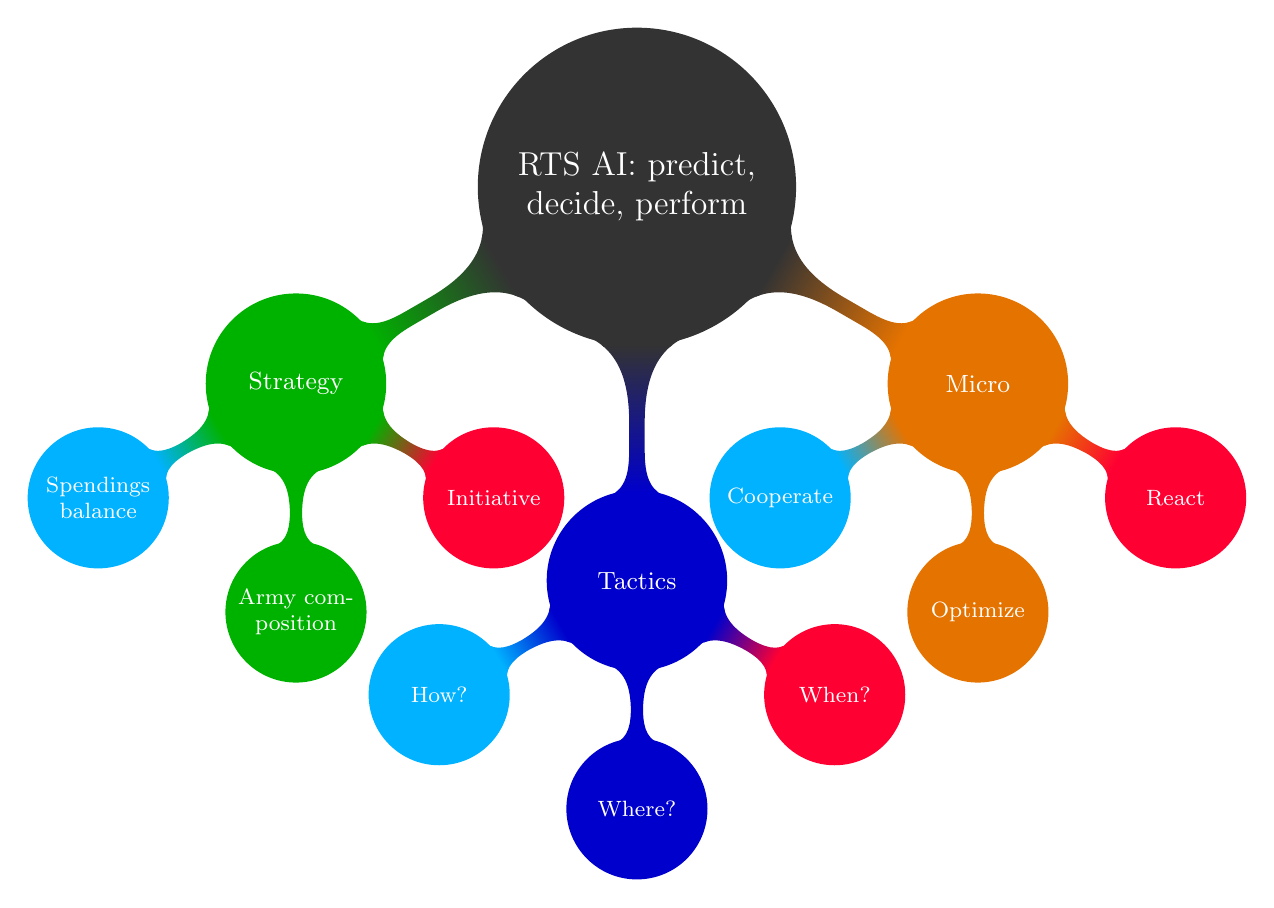
\begin{tikzpicture}
  \path[mindmap,concept color=black!80!white,text=white]
    node[concept] {RTS AI: predict, decide, perform}
    [clockwise from=-30]
    child[concept color=orange!90!black] {
      node[concept] {Micro}
      child[concept color=red!80!magenta] { node[concept] {React} }
      child { node[concept] {Optimize} }
      child[concept color=blue!30!cyan] { node[concept] {Cooperate} }
    }
    child[concept color=blue!80!black] { % TODO change color
      node[concept] {Tactics}
      child[concept color=red!80!magenta] { node[concept] {When?} }
      child { node[concept] {Where?} }
      child[concept color=blue!30!cyan] { node[concept] {How?} }
    }
    child[concept color=green!70!black] {
      node[concept] {Strategy}
      child[concept color=red!80!magenta] { node[concept] {Initiative} }
      child { node[concept] {Army composition} }
      child[concept color=blue!30!cyan] { node[concept] {Spendings balance} }
    };  
\end{tikzpicture}
\end{small}
\end{center}
\label{fig:mindmapRTS}
\caption{A mind-map of RTS AI XXX TODO}
\end{figure}

StarCraft subsumes Wargus, which has an estimated mean branching factor $1.5.10^3$ \citep{LTW} (Chess: $\approx 35$, Go: $<360$). \cite{bgweberPhD} find a branching factor of $> 1.10^6$ for StarCraft. The game complexity is roughly $10^11500$, versus the Shannon number for Chess ($10^43$).

\section{Task decomposition and linking}
\begin{figure}[!ht]
\begin{center}
\includegraphics[width=13cm]{images/starcraft_bbq_concept.pdf}
\end{center}
\label{fig:conceptbbq}
\caption{Information-centric view of the architecture of the major components of the bot. Arrows are labeled with the information or orders they convey: dotted arrows are convey constraints, double lined arrows convey distributions, plain and simple arrows convey direct information or orders. The gray parts perform game actions (as the physical actions of the player on the keyboard and mouse).}
\end{figure}

In Fig.~\ref{fig:conceptbbq}, we present the flow of informations between the different inference and decision-making parts of the bot architecture. One can also view this problem as having a good model of one's strategy, one's opponent strategy, and taking decisions. The software architecture that we propose is to have services building and maintaining the model of the enemy as well as our state, and decision-making modules using all this information to give orders to actuators.

\begin{itemize}
\item Problem: build a real-scale software piece which is maintainable
\item State of the art: shared memories, shared states
\item Our take: we transmit distributions, states stay in modules
\item Results: XXX (atm too much state), also competitions results
\end{itemize}

% XXX 
XXX Real-time strategy (RTS) gameplay consist in producing and managing group of units with attacks and movements specificities in order to defeat an enemy. Most often, it is required to gather resources and build up an economic and military power while expanding a technology tree. Parts of the map not in the sight range of the player's units are under \textit{\glos{fogofwar}}, so the player only has partial information about the enemy buildings and army. The way by which we expand the tech tree, the specific units composing the army, and the general stance (aggressive or defensive) form what we call \textit{strategy}. At the lower level, the actions performed by the player (human or not) to optimize the effectiveness of its units is called \textit{micro-management}. In between lies \textit{tactics}: where to attack, and how. A good human player takes much data in consideration when choosing: are there flaws in the defense? Which spot is more worthy to attack? How much am I vulnerable for attacking here? Is the terrain (height, chokes) to my advantage? etc.


\chapter{Micro-management}
\label{chapter:micro}
\begin{quotation}
\noindent
\textit{La vie est la somme de tous vos choix.
\vspace{0.2cm}\\
Life is the sum of all your choices.}
%\vspace{0.2cm}\\
\begin{flushright}Albert Camus\end{flushright}
\end{quotation}

\lettrine{W}{e} present a Bayesian sensory-motor model for multi-agent (decentralized) units control in an adversarial setting. Orders, coming from higher up in the decision hierarchy, are integrated as another sensory input. We evaluated our model on classic StarCraft \glos{micro} tasks. This work was published at Computational Intelligence in Games (CIG) 2011 in Seoul \citep{SYNNAEVE:Micro}.

\ifthenelse{\equal{\myebookformat}{false}}{
\chaptertoc
}{}
\newacronym{RL}{RL}{reinforcement learning}

\begin{itemize}
\item \underline{Problem:} optimal control of units in a (real-time) huge adversarial actions space (collisions, accelerations, terrain, damages, areas of effects, foes, goals...).
\item \underline{Problem that we solve:} efficient coordinated control of units incorporating all low level actions and inputs, plus higher level orders and representations.
\item \underline{Type:} it is a problem of \textit{multi-agent control in an adversarial environment}\footnote{Strictly, it can be modeled as a \glos{pomdp} for each unit independently with $S$ the states of all the other units (enemies and allied altogether) which are known through observations $O$ by conditional observations probabilities $\Omega$, with $A$ the set of actions for the given unit, $T$ transition probabilities between states and depending on actions, and the reward function $R$ based on goal execution, unit survivability and so on... It can also be viewed as a (gigantic) \glos{pomdp} solving the problem for all (controlled units) at once, the advantage is that all states $S$ for allied units is known, the disadvantage is that the combinatorics of $T$ and $A$ make it intractable for useful problems.}.
\item \underline{Complexity:} \textsc{pspace}-complete \citep{Papadimitriou87,GamingComplexity}. Our solutions are real-time on a laptop.
\end{itemize}

% TODO: 
% add graphical model??\\

\begin{figure}[ht]
\begin{center}
\includegraphics[width=13cm]{images/starcraft_bbq_concept_MICRO.pdf}
\end{center}
\caption{Information-centric view of the architecture of the bot, the part concerning this chapter (\glos{micro}) is in the dotted rectangle}
\label{fig:conceptMICRO}
\end{figure}

\section{Units Management}
\subsection{Micro-management complexity}
In this part, we focus on \glos{micro}, which is the lower-level in our hierarchy of decision-making levels (see Fig.~\ref{fig:starcraft_abstraction_time}) and directly affect units control/inputs. Micro-management consists in maximizing the effectiveness of the units \textit{i.e.} the damages given/damages received ratio. These has to be performed simultaneously for units of different types, in complex battles, and possibly on heterogeneous terrain. 
For instance: retreat and save a wounded unit so that the enemy units would have to chase it either boosts your firepower (if you save the unit) or weakens the opponent's (if they chase). 

StarCraft micro-management involves ground, flying, ranged, contact, static, moving (at different speeds), small and big units (see Figure~\ref{fig:sc_fight}). Units may also have splash damage, spells, and different types of damages whose amount will depend on the target size. It yields a rich states space and needs control to be very fast: human progamers can perform up to 400 ``actions per minute'' in intense fights. The problem for them is to know which actions are effective and the most rewarding to spend their actions efficiently. A robot does not have such physical limitations, but yet, badly chosen actions have negative influence on the issue of fights. %The problem is to identify what has to be done and what can be done, in real-time.

Let $\mathbf{U}$ be the set of the $m$ units to control, $\mathbf{A} = \{\cup_i\ \vec{d_i}\} \cup \mathbf{S}$ be the set of possible actions (all $n$ possible $\vec{d}$ directions, standing ground included, and $\mathbf{S}$kills, firing included), and $\mathbf{E}$ the set of enemies. As $|\mathbf{U}| = m$, we have $|\mathbf{A}|^{m}$ possible combinations each turn, and the enemy has $|\mathbf{A}|^{|\mathbf{E}|}$. 
The dimension of the set of possible actions each micro-turn (for instance: 1/24th of a second in StarCraft) constrains reasoning about the state of the game to be hierarchical, with different levels of granularity. In most RTS games, a unit can go (at least) in its 24 surrounding tiles (see Figure~\ref{fig:sc_fight}, each arrow correspond to a $\vec{d_i}$)
) %, combination of N, S, E, W up to the 2nd order), 
stay where it is, attack, and sometimes cast different spells: which yields more than 26 possible actions each turn. Even if we consider only 8 possible directions, stay, and attack, with $N$ units, there are $10^N$ possible combinations each turn (all units make a move each turn). As large battles in StarCraft account for \textit{at least} 20 units on each side, optimal units control hides in too big a search space to be fully explored in real-time (sub-second reaction at least) on normal hardware, even if we take only one decision per unit per second.

\begin{figure}
\begin{center}
\includegraphics[width=8.6cm]{images/SC_fight_3b.png}
\end{center}
\caption{Screen capture of a fight in which our bot controls the bottom-left units in StarCraft. The 25 possible directions ($\vec{d_1} \dots \vec{d_{25}}$) are represented for a unit with white and grey arrows around it. Orange lines represent units' targets, purple lines represent units' priority targets (which are objective directions in \textit{fightMove()} mode).}
\label{fig:sc_fight}
\end{figure}

\subsection{Our Approach}
Our full robot has separate agents types for separate tasks (strategy, tactics, economy, army, as well as enemy estimations and predictions): the part that interests us here, the unit control, is managed by Bayesian units directly. Their objectives are set by military goal-wise atomic units group, themselves spawned to achieve tactical goals (see Fig.~\ref{fig:conceptMICRO}). Units groups tune their Bayesian units modes (scout, fight, move) and give them objectives as sensory inputs. The Bayesian unit is the smallest entity and controls individual units as sensory-motor robots according to the model described above. The only inter Bayesian units communication about attack targets is handled by a structure shared at the units group level. This distributed sensory-motor model for \glos{micro} is able to handle both the complexity of unit control and the need of hierarchy (see Figure~\ref{fig:conceptMICRO}). We treat the units independently, thus reducing the complexity (no communication between our ``Bayesian units''), and allows to take higher-level orders into account along with local situation handling. For instance: the tactical planner may decide to retreat, or go through a choke under enemy fire, each Bayesian unit will have the higher-level order as a sensory input, along with topography, foes and allies positions. From its perception, our Bayesian robot \citep{Lebeltel04} can compute the distribution over its motor control. The performances of our models are evaluated against the original StarCraft AI and a reference AI (based on our targeting heuristic): they have proved excellent in this benchmark setup.


\section{Related Work}
Technical solutions include finite states machines (FSM) \citep{FSM}, genetic algorithms (GA) \citep{GA,Bakkes04,teamCompositionRTS}, reinforcement learning (RL) \citep{Marthi05concurrenthierarchical,Madeira06}, case-based reasoning (CBR) \citep{LTW,CBR-RL}, continuous action models \citep{Molineaux08}, reactive planning \citep{WeberCIG10}, upper confidence bounds tree (UCT) \citep{UCT}, potential fields \citep{Hagelback2009}, influence maps\citep{teamCompositionRTS}, and cognitive human-inspired models \citep{SORTS}.

FSM are well-known and widely used for control tasks due to their efficiency and implementation simplicity. However, they don't allow for state sharing, which increases the number of transitions to manage, and state storing, which makes collaborative behavior hard to code \citep{Cutumisu09}. Hierarchical FSM (HFSM) solve some of this problems (state sharing) and evolved into behavior trees (BT, hybrids HFSM) \citep{Isla} and behavior multi-queues (resumable, better for animation) \citep{Cutumisu09} that conserved high performances. %%%All these architectures does not include mechanisms to receive orders from separate entities. For instance, our strategic leader and tactical planners should be part of the (hierarchical) state machine, down to the control of units, which is not very flexible. 
However, adaptivity of behavior by parameters learning is not the main focus of these models, and unit control is a task that would require a huge amount of hand tuning of the behaviors to be really efficient. 
Also, these architectures does not allow reasoning under uncertainty, which helps dealing with local enemy and even allied units. Our agents see local enemy (and allied) units but do not know what action they are going to do. They could have perfect information about the allied units intentions, but this would need extensive communication between all the units.

Some interesting uses of \glos{RL} \citep{Sutton} to RTS research are concurrent hierarchical (units Q-functions are combined higher up) \glos{RL} \citep{Marthi05concurrenthierarchical} to efficiently control units in a multi-effector system fashion. \cite{Madeira06} advocate the use of prior domain knowledge to allow faster \glos{RL} learning and applied their work on a large scale (while being not as large as StarCraft) turn-based strategy game. In real game setups, \glos{RL} models have to deal with the fact that the state spaces to explore is enormous, so learning will be slow or shallow. It also requires the structure of the game to be described in a partial program (or often a partial Markov decision process) and a shape function \citep{Marthi05concurrenthierarchical}. RL can be seen as a transversal technique to learn parameters of an underlying model, and this underlying behavioral model matters. \cite{GA} used evolutionary learning techniques, but face the same problem of dimensionality. 

Case-based reasoning (CBR) allows for learning against dynamic opponents \citep{LTW} and has been applied successfully to strategic and tactical planning down to execution through behavior reasoning rules \citep{Ontanon2007}. CBR limitations (as well as RL) include the necessary approximation of the world and the difficulty to work with multi-scale goals and plans. These problems led respectively to continuous action models \citep{Molineaux08}and reactive planning \citep{WeberCIG10}. Continuous action models combine RL and CBR. Reactive planning use a decomposition similar to hierarchical task networks \citep{HTNPlanning} in that sub-plans can be changed at different granularity levels. Reactive planning allows for multi-scale (hierarchical) goals/actions integration and has been reported working on StarCraft, the main drawback is that it does not address uncertainty and so can not simply deal with hidden information (both extensional and intentional). 
Fully integrated FSM, BT, RL and CBR models all need vertical integration of goals, which is not very flexible (except in reactive planning).

Monte-Carlo planning \citep{Chung05} and upper Upper 
confidence bounds tree (UCT) planning (coming from Go AI) \citep{UCT} 
 samples through the (rigorously intractable) plans space by 
incrementally building the actions tree through Monte-Carlo sampling. 
UCT for tactical assault planning \citep{UCT} in RTS does not require to encode human knowledge (by opposition to Monte-Carlo planning) but it is too costly, both in learning and running time, to go down to units control on RTS problems. 
Our model subsumes potential fields \citep{Hagelback2009}, which are powerful and used in new generation RTS AI to handle threat, as some of our Bayesian unit sensory inputs are potential damages and tactical goodness (height for the moment) of positions. \cite{HagelbackJ08} presented a multi-agent potential fields based bot able to deal with fog of war in the Tankbattle game. \cite{Avery09} and \cite{SmithCIG10} co-evolved influence map trees for spatial reasoning in RTS games. \cite{Danielsiek_2008} used influence maps to achieve intelligent squad movement to flank the opponent in a RTS game. A drawback for potential field-based techniques is the large number of parameters that has to be tuned in order to achieve the desired behavior. 
Our model provides flocking and local (subjective to the unit) influences on the pathfinding as in \citep{teamCompositionRTS}, which uses self-organizing-maps (SOM). In their paper, Preuss \textit{et al.} are driven by the same quest for a more natural and efficient behavior for units in RTS. 
We would like to note that potential fields and influence maps are reactive control techniques, and as such, they do not perform any form of lookahead. In their raw form (without specific adaptation to deal with it), they can lead units to be stuck in local optimums (potential wells). 


Pathfinding is used differently in planning-based approaches and reactive approaches. \cite{Danielsiek_2008} is an example of the permeable interface between pathfinding and reactive control with influence maps augmented tactical pathfinding and flocking. As we used pathfinding as the mean to get a sensory input towards the objective, we were free to use a \textit{low resolution} and \textit{static} pathfinding for which A* was enough. Our approach is closer to the one of \citep{Reynolds_1999}: combining a simple path for the group with flocking behavior. In large problems and/or when the goal is to deal with multiple units pathfinding taking collisions (and sometimes other tactical features), more efficient, incremental and adaptable approaches are required. 
Even if specialized algorithms, such as D*-Lite \cite{KoenigL02} exist, it is most common to use A* combined with a map simplification technique that generates a simpler navigation graph to be used for pathfinding. An example of such technique is Triangulation Reduction A*, that computes polygonal triangulations on a grid-based map \cite{Demyen_2006}. In recent commercial RTS games like Starcraft 2 or Supreme Commander 2, flocking-like behaviors are inspired of continuum crowds (``flow field'') \cite{Treuille2006}. A comprehensive review about (grid-based) pathfinding was recently done by Sturtevant \cite{sturtevant2012benchmarks}.


Finally, there are some cognitive approaches to RTS AI \citep{SORTS}, and we particularly agree with Wintermute \textit{et al.} analysis of RTS AI problems. Our model has some similarities: separate agents for different levels of abstraction/reasoning and a perception-action approach (see Figure~\ref{fig:conceptMICRO}).

\section{A Pragmatic Approach to Units Control}
\subsection{Action and Perception}
\subsubsection{Movement}
The possible actions for each unit are to move from where they are to wherever on the map, plus to attack and/or use special abilities or spells. Atomic moves (shown in Fig.~\ref{fig:sc_fight} by white and gray plain arrows) correspond to move orders which will make the unit go in a straight line and \textit{not} call the pathfinder (if the terrain is unoccupied/free). There are collisions with buildings, other units, and the terrain (cliffs, water, etc.) which denies totally some movements for ground units. Flying units do not have any collision (neither with units, nor with terrain obviously). When a \textit{move order} is issued, if the selected position is further than atomic moves, the pathfinder function will be called to decide which path to follow. We decided to use only atomic (i.e. small and direct) moves for this reactive model, using other kinds of moves is discussed later in perspectives.

\subsubsection{Attacks}
To attack another unit, a given unit has to be in range (different attacks or abilities have different ranges) it has to have reloaded its weapon, which can be as quick as 4 times per second up to $\approx$3 seconds (75 frames) per attack. To cast a spell or use an ability also requires energy, which (re)generates slowly and can be accumulated up to a limited amount. Also, there are different kinds of attacks (normal, concussive, explosive), which modify the total amount of damages made on different types of units (small, medium, big), and different spread form and range of splash damages. Some spells/abilities absorb some damages on a given unit, others make a zone immune to all range attacks, etc. Finally, ranged attackers at a lower level (in terrain elevation) than their targets have an almost 50\% miss rate. These reasons make it an already hard problem just to select what to do without even moving. 

\subsubsection{Perceptions: potential damage map}
Perceptions are of different natures: either they are direct measurements inside the game, or they are built up from other direct measurements or even come from our AI higher level decisions. Direct measurements include the position of terrain elements (cliffs, water, space, trees). Built up measurements comes from composition of informations like the potential damage map (see Fig.~\ref{fig:potential_damage_map}. We maintain two (ground and air) damage maps which are built by summing all enemy units attack damages, normalized by their attack speed, for all positions which are in their range. These values are then discretized in levels $\{No, Low, Medium, High\}$ relative to the hit (health) points (HP) of the unit that we are moving. For instance, a tank (with many HP) will not fear going under some fire so he may have a $Low$ potential damages value for a given direction which will read as $Medium$ or $High$ for a light/weak unit like a marine. This will act as subjective potential fields \citep{Hagelback2009} in which the (repulsive) influence of the potential damages map depends on the unit type. The discrete steps are: 
$$\left\{0, \llbracket 0\dots \frac{unit\ base\ HP}{2}\rrbracket, \rrbracket \frac{unit\ base\ HP}{2} \dots unit\ base\ HP\llbracket, \llbracket unit\ base\ HP \dots +\inf\llbracket\right\}$$

\begin{figure}[h]
\begin{center}
\includegraphics[width=4cm]{images/tank_cac.png}
\hspace{1cm}
\includegraphics[width=4cm]{images/kiting.png}
\caption{Potential damage map (white squares for low potential damages, and yellow square for moderate potential damages). Left: we can see that the tank in siege mode (big blue unit with a red square on top) cannot shoot at close range and thus our units (in red) were attracted to the close safe zone. Right: the enemy units (blue, with red squares on top) are contact attack units and thus our unit (red, with a plain green square on top) is ``kiting'' (staying out of range): attacking and then retreating away (out of their range).}
\end{center}
\label{fig:potential_damage_map}
\end{figure}

\subsubsection{Repulsion/attraction}
For repulsion/attraction between units (allied or enemies), we could consider the instantaneous position of the units but it would lead to squeezing/expanding effects when moving large groups. Instead, we use their interpolated position at the time at which the unit that we move will be arrived in the direction we consider. In the right diagram in Figure~\ref{ fig:BayesianUnit_perceptions}, we want to move the unit in the center (\texttt{U}). There is an enemy (\texttt{E}) unit twice as fast as ours and an allied unit (\texttt{A}) three times as ours. When we consider moving in the direction just above us, we are on the interpolated position of unit \texttt{E} (we travel one case when they do two); when we consider moving in the direction directly on our right (East), we are on the interpolated position of unit \texttt{A}. 
We consider where the unit will be $\frac{\mathrm{dist}(unit, \vec{d_i})}{unit.speed}$ time later, but also its size (some units produce collisions in a smaller scale than our discretization).

\subsubsection{Objective}
The goals coming from the tactician model (see Fig.~\ref{fig:conceptMICRO}) are broken down into steps which gives objectives to each units. The way to incorporate the objective in the reactive behavior of our units is to add an attractive sensory input. This objective is a fixed direction $\vec{o}$ and we consider the probabilities of moving our unit in $n$ possible directions $\vec{d_1} \dots \vec{d_n}$ (in our StarCraft implementation: $n=25$ atomic directions). To decide the attractiveness of a given direction $\vec{d_i}$ with regard to the objective $\vec{o}$, we consider a weight which is proportional to the dot product $\vec{o} \cdot \vec{d_i}$, with a threshold minimum probability, as shown in Figure~\ref{fig:BayesianUnit_perceptions}.

\begin{figure}[h]
\begin{center}
\includegraphics[width=4.5cm]{images/repulsion_units_interpolation.pdf}
\hspace{1cm}
\includegraphics[width=4.5cm]{images/obj_Bayesian_units.pdf}
\caption{In both figures, the thick squares represents the boundaries of the 24 atomic directions (25 small squares with the current unit position) around the unit (\texttt{U}). Red is high probability, down to green low probability. Left: repulsion of the linear interpolation of the trajectories (here with uncertainty) of enemy unit (\texttt{E}) and allied unit (\texttt{A}), depending on their speed. Right: attraction of the objective (in direction of the dotted arrow) which is proportional to dot-product of the direction (square) considered, with a minimum threshold (in green).}
\label{fig:BayesianUnit_perceptions}
\end{center}
\end{figure}


\subsection{A Simple Unit}
\subsubsection{Greedy pragmatism}
Is staying alive better than killing an enemy unit? Is a large splash damage better than killing an enemy unit? Is it better to fire or move? In that event, where? Even if we could compute to the end of the fight and apply the same approach that we have for board games, how do we infer the best ``set of next moves'' for the enemy? %when the space of possible moves is so huge and the number of possible reasoning methods %(sacrifices and influences of other parts of the game for instance) 
%is bigger than for Chess? 
For enemy units, it would require exploring the tree of possible plans (intractable) whose we could at best only draw samples from \citep{UCT}. Even so, taking enemy minimax (to which depth?) moves for facts would assume that the enemy is also playing minimax (to the same depth) following exactly the same valuation rules as ours. Clearly, RTS \glos{micro} is more inclined to reactive planning than board games reasoning. That does not exclude having higher level (strategic and tactic) goals. In our model, they are fed to the unit as sensory inputs, that will have an influence on its behavior depending on the situation/state the unit is in. 
We should at least have a model for higher-level decisions of the enemy and account for uncertainty of moves that could be performed in this kind of minimax approach. So, as complete search through the min/max tree is intractable, we propose a first simple solution: have a greedy target selection heuristic leading the movements of units to benchmark our Bayesian model against. In this solution, each unit can be viewed as an effector, part of a multi-body (multi-effector) agent, grouped under a units group. 

\subsubsection{Targeting heuristic}
The idea behind the heuristic used for target selection is that units need to focus fire (which leads to less incoming damages if enemy units die faster) on units that do the most damages, have the less hit points, and take the most damages from their attack type. This can be achieved by using a data structure, shared by all our units engaged in the battle, that stores the damages corresponding to future allied attacks for each enemy units. Whenever a unit will fire on a enemy unit, it registers there the future damages on the enemy unit. As attacks are not all instantaneous and there are reload times, it helps focus firing greatly\footnote{The only degenerated case would be if all our units register their targets at once (and all the enemy units have the same priority) and it never happens (plus, units fire rates have a randomness factor).}. 
We also need a set of priority targets for each of our unit types that can be drawn from expert knowledge or learned (reinforcement learning) battling all unit types. A unit select its target among the most focus fired units with positive future hit point (current hit points minus registered damages), while prioritizing units from the priority set of its type. The units group can also impose its own priorities on enemy units (for instance to achieve a goal). The target selection heuristics is fully depicted in \ref{alg:targetselection} in the appendices.

\subsubsection{Fight behavior}
\label{sec:HOAI}
Based on this targeting heuristic, we design a very simple FSM based unit as shown in Figure~\ref{fig:fight_FSM} and Algorithm~\ref{alg:fight_FSM}: when the unit is not firing, it will either flee damages if it has taken too much damages and/or if the differential of damages is too strong, or move to be better positioned in the fight (which may include staying where it is). In this simple unit, the \textit{flee()} function just tries to move the unit in the direction of the biggest damages gradient (towards lower potential damages zones). The \textit{fightMove()} function tries to position the units better: in range of its priority target, so that if the priority target is out of reach, the behavior will look like: ``try to fire on target in range, if it cannot (reloading or no target in range), move towards priority target''. As everything is driven by the firing heuristic (that we will also use for our Bayesian unit), we call this AI the Heuristic Only AI (HOAI).

\begin{figure}[h]
\begin{algorithmic}
\Function{move}{$prio\_t, \nabla dmg$}
\If {$needFlee()$}
    \State {$flee(\nabla dmg)$}
\Else
    \State {$fightMove(prio\_t)$}
\EndIf
\EndFunction

\Function{fight}{}
\State $(target, prio\_target) = selectTarget()$
\If {$reloaded$}
    \If {$inRange(prio\_target)$}
        \State {$attack(prio\_target)$}
    \ElsIf {$inRange(target)$}
        \State {$attack(target)$}
    \Else
        \State {$move(prio\_target, damage\_gradient)$}
    \EndIf
\Else
    \State {$move(prio\_target, damage\_gradient)$}
\EndIf
\EndFunction
\end{algorithmic}
\caption{Fight behavior FSM for micro-managing units.}
\label{alg:fight_FSM}
\end{figure}

\begin{figure}[h]
\begin{center}
\includegraphics[width=5.5cm]{images/simple_unit_fight_FSM.pdf}
\end{center}
\caption{Fight FSM of a simple unit model: Heuristic Only AI (HOAI), which will serve as a baseline for benchmarks.}
\label{fig:fight_FSM}
\end{figure}


\subsection{Units Group}

\label{section:unitsgroup}
The units group (\texttt{UnitsGroup}, see Fig.~\ref{fig:conceptMICRO}) makes the shared \textit{future damage} data structure available to all units taking part in a fight. Units control is not limited to fight. As it is adversarial, it is perhaps the hardest task, but units control problems comprehends efficient team manoeuvering and other behaviors such as scouting or staying in position (formation). The units group structure helps for all that: it decides of the modes in which the unit has to be. We implemented 4 modes in our Bayesian unit (see Fig.~\ref{fig:unit_HFSM}): \textit{fight, move, scout, inposition}. When given a task, also named goal, by the tactician model (see Fig.~\ref{conceptMICRO}), the units group has to transform the task objective into sensory inputs for the units. 
\begin{itemize}
    \item In \textit{scout} mode, the (often quick and low hit points) unit avoids danger by modifying locally its pathfinding-based, objectives oriented route to avoid damages.
    \item In \textit{move} mode, the objective is extracted for the pathfinder output: it consists in key waypoints near the units. When moving by flocking, our unit moves are influenced by other near allied units that repulse or attract it depending on its distance to the interpolation of the allied unit. It allows our units to move more efficiently by not splitting around obstacles and colliding less. As it causes other problems, we do not use the flocking behavior in full competitive games.
    \item In the \textit{inposition} mode, the objective is the final unit formation position. The unit can be ``pushed'' by other units wanting to pass through. This is useful at a tactical level to do a wall of units that our units can traverse but the opponent's cannot. Basically, there is an attraction to the position of the unit and a stronger repulsion of the interpolation of movements of allied units.
    \item In \textit{fight} mode, our unit will follow the damages gradient to smart positions, for instance close to tanks (they cannot fire too close to their position) or far from too much contact units if our unit can attack with range (something called ``kiting''). Our unit moves are also influenced by its priority targets, its goal/objective (go through a choke, flee, etc.) and other units. The objective depends of the confidence of the units group in the outcome of the battle:
\begin{itemize}
    \item If the units group is outnumbered (in adjusted strength) and the task is not a suicidal one, the units group will ``fall back'' and give objectives towards retreat. 
    \item If the fight is even or manageable, the units group will not give any objective to units, which will set their own objectives either to their priority targets in \textit{fightMove()} or towards fleeing damages (towards highest potential damages gradient) in \textit{flee()}.
    \item If the units group is very confident in winning the fight, the objectives sensory inputs of the units will be set at the task objectives waypoints (from the pathfinder).
\end{itemize}
\end{itemize} 

\section{A Bayesian Model for Units Control}

\label{sec:bayesianunit}
\subsection{Bayesian Unit}

We use Bayesian programming as an alternative to logic, transforming incompleteness of knowledge about the world into uncertainty. In the case of units management, we have mainly \textit{intensional} uncertainty. Instead of asking questions like: where are other units going to be 10 frames later? Our model is based on rough estimations that are not taken as ground facts. Knowing the answer to these questions would require for our own (allied) units to communicate a lot and to stick to their plan (which does not allow for quick reaction nor adaptation). 

We propose to model units as sensory-motor robots described within the Bayesian robot programming framework \citep{Lebeltel04}. A Bayesian model uses and reasons on distributions instead of predicates, which deals directly with uncertainty. %Basically, a Bayesian unit will be attracted or repulsed by its sensory inputs. 
Our Bayesian units are simple hierarchical finite states machines (states can be seen as modes) that can scout, fight and move (see Figure~\ref{fig:unit_HFSM}). Each unit type has a reload rate and attack duration, so their fight mode will be as depicted in Figure~\ref{fig:fight_FSM} and Algorithm~\ref{alg:fight_FSM}. The difference between our simple HOAI presented above and Bayesian units are in \textit{flee()} and \textit{fightMove()} functions.
\begin{figure}[h]
\begin{center}
\includegraphics[width=7cm]{images/unit_HFSM2.pdf}
\end{center}
\caption{Bayesian unit modal FSM, detail on the fight mode. Stripped modes are Bayesian.}
\label{fig:unit_HFSM}
\end{figure}

The unit needs to determine where to go when fleeing and moving during a fight, with regard to its target and the attacking enemies, while avoiding collisions (which results in blocked units and time lost) as much as possible. \textbf{We now present the Bayesian program used for \textit{flee()}, \textit{fightMove()}, and while scouting}, which differ only by what is inputed as objective:
\subsubsection{Variables}
\begin{itemize}
\item $Dir_{i \in \llbracket 1 \dots n\rrbracket } \in \{True, False\}$: at least one variable for each atomic direction the unit can go to. $\PP(Dir_i = True) = 1$ means that the unit will certainly go in direction $i$ ($\Leftrightarrow \vec{d_i}$). For example, in StarCraft we use the 24 atomic directions (48 for the smallest and fast units as we use a proportional scale) plus the current unit position (stay where it is) as shown in Figure~\ref{fig:sc_fight}. %We could use one variable with 24 directions, the approach would be the same. %%% Note that $i \in \llbracket 1 \dots n\rrbracket \Leftrightarrow \mathbf{D}[i] \in \mathbf{D}$.

\item $Obj_{i \in \llbracket 1 \dots n\rrbracket } \in \{True, False\}$: adequacy of direction $i$ with the objective (given by a higher rank model). In our StarCraft AI, we use the scalar product between the direction $i$ and the objective vector (output of the pathfinding) with a minimum value ($0.3$ in \textit{move} mode for instance) so that the probability to go in a given direction is proportional to its alignment with the objective.
\begin{itemize}
    \item For \textit{flee()}, the objective is set in the direction which flees the potential damage gradient (corresponding to the unit type: ground or air).
    \item For \textit{fightMove()}, the objective is set (by the units group) either to retreat, to fight freely or to march aggressively towards the goal (see \ref{section:unitsgroup}).
    \item For the \textit{scout} behavior, the objective ($\vec{o}$) is set to the next pathfinder waypoint.
\end{itemize}

\item $Dmg_{i \in \llbracket 1 \dots n\rrbracket } \in \{no, low, medium, high\}$: potential damage value in direction $i$, relative to the unit base health points, in direction $i$. In our StarCraft AI, this is directly drawn from two constantly updated potential damage maps (air, ground). %For instance, it allows our scouting units to avoid potential attacks as much as possible.

\item $A_{i \in \llbracket 1 \dots n\rrbracket } \in \{free, small, big\}$: occupation of the direction $i$ by an allied unit. The model can effectively use many values (other than ``occupied/free'') because directions may be multi-scale (for instance we indexed the scale on the size of the unit) and, in the end, small and/or fast units have a much smaller footprint, collision wise, than big and/or slow. In our AI, instead of direct positions of allied units, we used their (linear) interpolation $\frac{\mathrm{dist}(unit, \vec{d_i})}{unit.speed}$ (time it takes the unit to go to $\vec{d_i}$) 
frames later (to avoid squeezing/expansion).

\item $E_{i \in \llbracket 1 \dots n\rrbracket } \in \{free, small, big\}$: occupation of the direction $i$ by an enemy unit. As above.

\item $Occ_{i \in \llbracket 1 \dots n\rrbracket } \in \{free, building, staticterrain\}$%(this could have been 2 variables or we could omit static terrain but we stay as general as possible): 
: Occupied, repulsive effect of buildings and terrain (cliffs, water, walls).
\end{itemize}

There is basically one set of (sensory) variables per perception in addition to the $Dir_i$ values. 

\subsubsection{Decomposition}

The joint distribution ($JD$) over these variables is a specific kind of fusion called inverse programming \citep{LeHy04}. The sensory variables are considered conditionally independent knowing the actions, contrary to standard naive Bayesian fusion, in which the sensory variables are considered independent knowing the phenomenon.
\begin{eqnarray}
&& \PP(Dir_{1:n}, Obj_{1:n}, Dmg_{1:n}, A_{1:n}, E_{1:n}, Occ_{1:n})\\
& = & JD = \prod_{i=1}^{n} \PP(Dir_i) \PP(Obj_i | Dir_i) \\
                    && \PP(Dmg_i | Dir_i) \PP(A_i | Dir_i) \\
                    && \PP(E_i | Dir_i) \PP(Occ_i | Dir_i)
\end{eqnarray}
We assume that the $i$ directions are independent depending on the action because dependency is already encoded in (all) sensory inputs. 

\subsubsection{Forms}

\begin{itemize}
\item $\PP(Dir_i)$ prior on directions, unknown, so unspecified/uniform over all $i$. $\PP(dir_i) = 0.5$.

\item $\PP(Obj_i | Dir_i)$ for instance, ``probability that this direction is the objective knowing that we go there'' $\PP(obj_i | dir_i) = threshold + (1.0-threshold)\times \mathrm{max}(0, vec{o} \cdot \vec{d_i})$. %$\PP(Obj_i = T | Dir_i = T)$ is very high (close to one) when rushing towards an objective, whereas it is far less important when fleeing. 
We could have different $thresholds$ depending on the mode, this was not the case in our hand-specified tables: $threshold = 0.3$. The right diagram on Figure~\ref{fig:BayesianUnit_perceptions} shows $\PP(Obj_i|Dir_i)$ for each for the possible directions (inside the thick big square boundaries of atomic directions) with red being higher probabilities.

\item $\PP(Dmg_i | Dir_i)$ probability of damages values in direction $i$ knowing this is the direction that we are headed to. $\PP(Dmg_i = high | Dir_i = T)$ has to be small in many cases for the unit to avoid going to positions it could be killed instantly. Probability table:\\
\begin{center}
\begin{tabular}{|l|c|c|}
\hline
$Dmg_i$ & $dir_i$ & $\bar{dir_i}$ \\
\hline
no & 0.9 & 0.25 \\
low & 0.06 & 0.25 \\
medium & 0.03 & 0.25 \\
high & 0.01 & 0.25 \\
\hline
\end{tabular}
\end{center}

\item $\PP(A_i | Dir_i)$ probability that there is an ally in direction $I$ knowing this is the unit direction. It is used to avoid collisions by not going where allied units could be in the near future. Probability table:\\
\begin{center}
\begin{tabular}{|l|c|c|}
\hline
$A_i$ & $dir_i$ & $\bar{dir_i}$ \\
\hline
free & 0.9 & 0.333 \\
small & 0.06 & 0.333 \\
big & 0.03 & 0.333 \\
\hline
\end{tabular}
\end{center}
 

\item $\PP(E_i | Dir_i)$ same explanation and use as above but with enemy units, it can have different parameters as we may want to be stucking enemy units, or avoid them (mostly depending on the unit type). In a repulsive setting (what we mostly want), the left diagram in Figure~\ref{fig:BayesianUnit_perceptions} can be seen as $\PP(A_i,E_i | \bar{Dir_i})$ if red corresponds to high probabilities ($\PP(A_i,E_i|Dir_i)$ if red corresponds to lower probabilities). In our hand-specified implementation, for \textit{flee()} and \textit{fightMove()}, this is the same probability table as above (for $\PP(A_i | Dir_i)$).

\item $\PP(Occ_i | Dir_i)$ probability table that there is a blocking building or terrain element is some direction, knowing this is the unit direction, $\PP(Occ_i = Static | Dir_i = T)$ will be very low, whereas $\PP(Occ_i = Building | Dir_i = T)$ will also be very low but triggers building attack (and destruction) when there are no other issues.
Probability table:\\
\begin{center}
\begin{tabular}{|l|c|c|}
\hline
$Occ_i$ & $dir_i$ & $\bar{dir_i}$ \\
\hline
free & 0.999899 & 0.333 \\
building & 0.001 & 0.333 \\
static & 0.000001 & 0.333 \\
\hline
\end{tabular}
\end{center}

\end{itemize}



\subsubsection{Identification}

Parameters and probability tables can be learned through reinforcement learning \citep{Sutton,Asmuth09} by setting up different and pertinent scenarii and search for the set of parameters that maximizes a reward function (more about that in the discussion). In our current implementation, the parameters and probability table values are hand specified.

\subsubsection{Question}

When in \textit{fightMove()} and \textit{flee()}, the unit asks:
\begin{equation}
\PP(Dir_{1:n} | Obj_{1:n}, Dmg_{1:n}, A_{1:n}, E_{1:n}, Occ_{1:n}, Prio_{1:n})
\end{equation}

From there, the unit can either go in the most probable $Dir_i$ or sample through them. We describe the effect of this choice in the next section (and in Fig.~\ref{fig:BayesianUnitChoice}). A simple Bayesian fusion from 3 sensory inputs is shown in Figure~\ref{fig:BayesianUnitExample}, in which the final distribution on $Dir$ peaks at places avoiding damages and collisions while pointing towards the goal. Here follows the full Bayesian program of the model (\ref{bp:BayesianUnit_fightmove}):

\begin{figure}[h]
\begin{center}
\includegraphics[width=13cm]{images/example_BayesianUnit.pdf}
\end{center}
\caption{Simple example of Bayesian fusion from 3 sensory inputs (damages and collisions avoidance, goal attraction). The grid pattern represents statically occupied terrain, the unit we control is in \texttt{U}, an allied unit is in \texttt{A}. The result is displayed on the rightmost image.}
\label{fig:BayesianUnitExample}
\end{figure}

\begin{figure}[!h]
\begin{eqnarray*}
\begin{sideways}\parbox{35mm}{\hspace{-1.3cm}Bayesian program}\end{sideways}
\begin{cases}
\begin{sideways}\parbox{15mm}{\hspace{-0.8cm}Description}\end{sideways}
    \begin{cases}
\begin{sideways}\parbox{18mm}{\hspace{-1.1cm}Specification ($\pi$)}\end{sideways}
        \begin{cases}
        Variables\\
Dir_{1:n}, Obj_{1:n}, Dmg_{1:n}, A_{1:n}, E_{1:n}, Occ_{1:n} \\
        Decomposition\\
 \PP(Dir_{1:n}, Obj_{1:n}, Dmg_{1:n}, A_{1:n}, E_{1:n}, Occ_{1:n}) =  \prod_{i=1}^{n} \big[ \PP(Dir_i) \\
 \PP(Obj_i | Dir_i) \PP(Dmg_i | Dir_i) \PP(A_i | Dir_i) \PP(E_i | Dir_i) \PP(Occ_i | Dir_i)\big]\\
        Forms\\
\PP(Dir_i): \mathrm{prior\ on\ directions\ (crossing\ policy)} \\
\PP(XYZ_i | Dir_i):\ \mathrm{probability\ tables}\\
        \end{cases}\\
    Identification\ (using\ \delta)\\
\mathrm{reinforcement\ learning\ or\ hand\ specified\ (or\ distribs.\ parameters\ optimization)}
    \end{cases}\\
Question\\
 \mathrm{fight moving/fleeing/scouting:}\ \ \PP(Dir_{1:n} | Obj_{1:n}, Dmg_{1:n}, A_{1:n}, E_{1:n}, Occ_{1:n}, Prio_{1:n})\\
%%%  \mathrm{fleeing:}\ \  \PP(Dir_{1:n} | Obj_{1:n}, Dmg_{1:n}, A_{1:n}, E_{1:n}, Occ_{1:n})\\
%%%  \mathrm{flocking:}\ \  \PP(Dir_{1:n} | Obj_{1:n}, Dmg_{1:n}, A_{1:n}, E_{1:n}, Occ_{1:n}, Att_{1:n,1:m})\\
\end{cases}
\end{eqnarray*}
\label{bp:BayesianUnit_fightmove}
\end{figure}

There are additional variables for specific modes/behaviors, also probability tables may be different.

\subsubsection{Move}

\noindent\textit{Without flocking}\\
When moving without flocking (trying to maintain some form of group cohesion), the model is even simpler. The objective ($\vec{o}$) is set to a path waypoint. The potential damage map is dropped from the $JD$, the question is:
\begin{equation}
\PP(Dir_{1:n} | Obj_{1:n}, A_{1:n}, E_{1:n}, Occ_{1:n})
\end{equation}

\noindent\textit{With flocking}\\
%To produce a \textit{flocking} behavior while moving, with $m$ units, we introduce another set of variables: $Att_{i \in \llbracket 0 \dots n\rrbracket, j \in \llbracket 0 \dots m \rrbracket} \in \{too\_close, near, far, too\_far\}$\footnote{the discrete levels could be replaced by the distance and $\PP(Att_{i,j}|Dir_i)$ could use a $Beta(\alpha, \beta)$ distribution with $\beta > \alpha > 1$.}, allied units attractions and repulsions. 
%Different than $A_i$, the $JD$ would become $JD \times \Pi_{i=1}^{n} \Pi_{j=1}^{m} \PP(Att_{i,j} | Dir_i)$, where $\PP(Att_{i,j} | Dir_i)$\footnote{Changing for $\PP(Att_i|Dir_i)P(Dir_i)$ for $\PP(Dir_i|Att_i)$ may be easier to reason about.} is a probability table for flocking: a too close unit $j$ will repel the Bayesian unit ($\PP(Att_{i,j} | Dir_i) < mean$) whereas another unit $j$ will attract depending on its distance (and possibly, leadership).
To produce a \textit{flocking} behavior while moving, we introduce another set of variables: $Att_{i \in \llbracket 1 \dots n\rrbracket} \in \{True,False\}$, allied units attractions (or not) in direction $i$.

A flocking behavior \citep{Reynolds_1999} requires:
\begin{itemize}
    \item Separation: avoid collisions, short range repulsion,
    \item Alignment: align direction with neighbours,
    \item Cohesion: steer towards average position of neighbours.
\end{itemize}
Separation is dealt with by $\PP(A_i|Dir_i)$ already. As we use interpolations of units at the time at which our unit will be arrived at the $Dir_i$ under consideration, being attracted by $Att_i$ gives cohesion as well as some form of alignment. It is not strictly the same as having the same direction and seems to fare better is complex terrain. We remind the reader that flocking was derived from birds flocks and fish schools behaviors: in both cases there is a lot of free/empty space.

A $\vec{a}$ vector is constructed as the weighted sum of neighbour\footnote{The devil is in the details, if one considers a too small neighbourhood, there is very rarely emergence of the flocking behavior, whereas if one considers a too large neighbourhood, units can get in directions which are stucking them with terrain. A pragmatic solution is to use a large neighbourhood with a decreasing weight (for increasing distance) for each unit of the neighbourhood.} allied units. Then $\PP(Att_i|Dir_i)$%\footnote{Changing for $\PP(Att_i|Dir_i)P(Dir_i)$ for $\PP(Dir_i|Att_i)$, with $Att_i$ being the distance, may be easier to reason about.}
 for all $i$ directions is constructed as for the objective influence ($\PP(Obj_i|Dir_i)$) by taking the dot product $\vec{a} \cdot \vec{d_i}$ with a minimum threshold (we used 0.3, so that the flocking effect is as strong as objective attraction):
$$\PP(att_i|dir_i) = threshold + (1.0-threshold)\times \mathrm{max}(0, \vec{a} \cdot \vec{d_i})$$

The $JD$ becomes $JD \times \Pi_{i=1}^{n} \PP(Att_{i} | Dir_i)$.
%%% \begin{center}
%%% \begin{tabular}{|l|c|c|}
%%% \hline
%%% $Att_{i,j}$ & $dir_i$ & $\bar{dir_i}$ \\
%%% \hline
%%% close & 0.4 & 0.5 \\
%%% far & 0.5 & 0.05 \\
%%% too\_far & 0.1 & 0.9 \\
%%% \hline
%%% \end{tabular}
%%% \end{center}

\begin{figure}[h]
\begin{eqnarray*}
\begin{sideways}\parbox{35mm}{\hspace{-1.3cm}Bayesian program}\end{sideways}
\begin{cases}
\begin{sideways}\parbox{15mm}{\hspace{-0.8cm}Description}\end{sideways}
    \begin{cases}
\begin{sideways}\parbox{18mm}{\hspace{-1.1cm}Specification ($\pi$)}\end{sideways}
        \begin{cases}
        Variables\\
Dir_{1:n}, Obj_{1:n}, Att_{1:n}, A_{1:n}, E_{1:n}, Occ_{1:n} \\
%Dir_{1:n}, Obj_{1:n}, Att_{1:n,1:m}, A_{1:n}, E_{1:n}, Occ_{1:n} \\
        Decomposition\\
 \PP(Dir_{1:n}, Obj_{1:n}, Att_{1:n}, A_{1:n}, E_{1:n}, Occ_{1:n}) =  \prod_{i=1}^{n} \big[ \PP(Dir_i) \\
% \PP(Dir_{1:n}, Obj_{1:n}, Att_{1:n,1:m}, A_{1:n}, E_{1:n}, Occ_{1:n}) =  \prod_{i=1}^{n} \big[ \PP(Dir_i) \\
 \PP(Obj_i | Dir_i) \PP(A_i | Dir_i) \PP(E_i | Dir_i) \PP(Occ_i | Dir_i)
\PP(Att_{i} | Dir_i)
%\prod_{j=1}^{m} \PP(Att_{i,j} | Dir_i)
\big]\\
        Forms\\
\PP(Dir_i): \mathrm{prior\ on\ directions\ (crossing\ policy)} \\
\PP(XYZ_i | Dir_i):\ \mathrm{probability\ tables}\\
        \end{cases}\\
    Identification\ (using\ \delta)\\
\mathrm{learning\ or\ hand\ specified}\\
    \end{cases}\\
Question\\
 \mathrm{flocking:}\ \  \PP(Dir_{1:n} | Obj_{1:n}, A_{1:n}, E_{1:n}, Occ_{1:n}, Att_{1:n})\\
% \mathrm{flocking:}\ \  \PP(Dir_{1:n} | Obj_{1:n}, A_{1:n}, E_{1:n}, Occ_{1:n}, Att_{1:n,1:m})\\
\end{cases}
\end{eqnarray*}
\label{bp:BayesianUnit_move}
\end{figure}


\subsubsection{In position}

%\item $Prio_{i \in \llbracket 1 \dots n\rrbracket } \in \{True, False\}$: combined effect of the priority targets that attract the unit while in fight ($fightMove()$). The $JD$ is modified as $JD \times \Pi_{i=1}^{n} \PP(Prio_i | Dir_i)$, where $\PP(Prio_i | Dir_i)$ is a probability table, that corresponds to the attraction of a priority (maybe out of range) target in this direction. This is efficient to be able to target casters or long range units for instance.
The \textit{inposition} mode corresponds to when some units are at the place they should be (no new objective to reach) and not fighting. This happens when some units arrived at their formation end positions and they are waiting for other (allied) units of their group, or when units are sitting (in defense) at some tactical point, like in front of a base for instance. The particularity of this mode is that the objective is set to the current unit position and it will be updated to always point to this ``final formation position'' as long as the unit is in this mode. This is useful so that units which are arriving to the formation can go through each others and not get stuck. Figure~\ref{fig:squaretraversal} shows the effect of using this mode: the big unit (Archon) goes through a square formation of the other units (Dragoons) which are in \textit{inposition} mode. What happens is an emerging phenomenon: the first (leftmost) units of the square get repulsed by the interpolated position of the dragoon, so they move themselves out of its trajectory. By moving, they repulse the second and then third line of the formation, the chain repulsion reaction makes a path for the big unit to pass through the formation. Once this unit path is no longer colliding, the attraction of units for their objective (their formation position) takes them back to their initial positions.

\begin{figure}[h]
\begin{center}
\begin{tabular}{cc}
\includegraphics[width=7.5cm]{images/square_traversal_1.png} & 
\includegraphics[width=7.5cm]{images/square_traversal_2.png} \\
\includegraphics[width=7.5cm]{images/square_traversal_3.png} & 
\includegraphics[width=7.5cm]{images/square_traversal_4.png} \\
\end{tabular}
\caption{Sequence of traversal of an Archon (big blue unit which is circled in green) through a square formation of Dragoons (four legged red units) in \textit{inposition} mode.}
\label{fig:squaretraversal}
\end{center}
\end{figure}


\section{Results on StarCraft}

Our implementation\footnote{\textsc{BroodwarBotQ}, code and releases: \url{http://github.com/SnippyHolloW/BroodwarBotQ}} (BSD licensed) uses BWAPI\footnote{BWAPI: \url{http://code.google.com/p/bwapi/}} to get information from and to control StarCraft. 

\subsection{Experiments}

We produced three different AI to run experiments with, along with the original AI (OAI) from StarCraft:
\begin{itemize}
\item Heuristic only AI (HOAI), as described above (\ref{sec:HOAI}): this AI shares the target selection heuristic with our Bayesian AI models and will be used as a baseline reference to avoid the bias due to the target selection heuristic.
\item Bayesian AI picking best (BAIPB): this AI follows the model of section~\ref{sec:bayesianunit} and selects the most probable $Dir_i$ as movement. 
\item Bayesian AI sampling (BAIS): this AI follows the model of section~\ref{sec:bayesianunit} and samples through $Dir_i$ according to their probability (i.e. it samples a direction in the $Dir$ distribution).
\end{itemize}

The experiments consisted in having the AIs fight against each others on a micro-management scenario with mirror matches of 12 and 36 ranged ground units (Dragoons). In the 12 units setup, the unit movements during the battle is easier (less collision probability) than in the 36 units setup. We instantiate only the army manager (no economy in this special scenarii/maps), one units group manager and as many Bayesian units as there are units provided to us in the scenario. The results are presented in Table~\ref{tab:win_ratios}.

\definecolor{grey}{rgb}{0.7,0.7,0.7}
\begin{table}[h]
\begin{center}
\begin{tabular}{|l|c|c|c|c|}
\hline
12 units & OAI & HOAI & BAIPB & BAIS \\
\hline
OAI & (50\%) & & & \\
HOAI & 59\% & (50\%) & & \\
BAIPB & 93\% & 97\% & (50\%) & \\
BAIS & 93\% & 95\% & 76\% & (50\%)\\
\hline
\end{tabular}
\begin{tabular}{|l|c|c|c|c|}
\hline
36 units & OAI & HOAI & BAIPB & BAIS \\
\hline
OAI & (50\%) & & & \\
HOAI & 46\% & (50\%) & & \\
BAIPB & 91\% & 89\% & (50\%) & \\
BAIS & 97\% & 94\% & 97\% & (50\%)\\
\hline
\end{tabular}
\end{center}
% BAIPB+Heuristics flee/fightmove 12 goons vs OAI 94/100
% BAIPB+Heuristics flee/fightmove 36 goons vs OAI 95/100
% pure BAIPB (fightMove only on ``potential fields'') 12 goons vs OAI 51/33
% pure BAIPB (fightMove only on ``potential fields'') 36 goons vs OAI 10/16
%%%\caption{Win ratios over at least 200 battles of the Original AI (OAI), Heuristic Only AI (HOAI), Bayesian AI Pick Best (BAIPB) and Bayesian AI Sample (BAIS) in two mirror setups: 12 and 36 ranged units. Read line vs column: for instance HOAI won 59\% of its matches against OAI in the 12 units setup. Note: The average amount of units left at the end of battles is proportional to the percentage of wins.}
\caption{Win ratios over at least 200 battles of OAI, HOAI, BAIPB and BAIS in two mirror setups: 12 and 36 ranged units. Left: 12 units (12 vs 12) setup. Right: 36 units (36 vs 36) setup. Read line vs column: for instance HOAI won 59\% of its matches against OAI in the 12 units setup.} %Note: The average amount of units left at the end of battles is grossly proportional to the percentage of wins.}
\label{tab:win_ratios}
\end{table}

These results show that our heuristic (HAOI) is comparable to the original AI (OAI), perhaps a little better, but induces more collisions as we can see its performance diminish a lot in the 36 units setup vs OAI. For Bayesian units, the ``pick best'' (BAIPB) direction policy is very effective when battling with few units (and few movements because of static enemy units) as proved against OAI and HOAI, but its effectiveness decreases when the number of units increases: all units are competing for the best directions (to $flee()$ or $fightMove()$ in) and they collide. The sampling policy (BAIS) has way better results in large armies, and significantly better results in the 12 units vs BAIPB. BAIPB may lead our units to move inside the ``enemy zone'' a lot more to chase priority targets (in \textit{fightMove()}) and collide with enemy units or get kill. Sampling entails that the competition for the best directions is distributed among all the ``bests to good'' positions, from the units point of view. We illustrate this effect in Figure~\ref{fig:BayesianUnitChoice}: the units (on the right of the figure) have good reasons (combinations of sensory inputs, for instance of the damage map) to flee on the left, and there may be a peak of ``best position to be at''. AS they have not moved yet, they do not have interpolation of positions which will collide, so they are not repulsing each other at this position, all go together and collide. Sampling would, on average, provide a collision free solution here.
\begin{figure}[h]
\includegraphics[width=12cm]{images/distDir.png}
\hspace{0.8cm}
\includegraphics[width=2.6cm]{images/flee_sample.png}
\caption{Example of $\PP(Dir)$ when fleeing, showing why sampling (BAIS, bottom graphic on the right) may be a better instead of picking the best direction (BAIPB, here $Dir=17$ in the plot, top graphic on the right) and triggering units collisions.}
\label{fig:BayesianUnitChoice}
\end{figure}

We also ran tests in setups with flying units (Zerg Mutalisks) in which BAIPB fared as good as BAIS (no collision for flying units) and way better than OAI.

\subsection{Our bot}

This model is currently at the core of the micro-management of our StarCraft bot. In a competitive micro-management setup, we had a tie with the winner of AIIDE 2010 StarCraft micro-management competition, winning with ranged units (Protoss Dragoons), losing with contact units (Protoss Zealots) and having a perfect tie (the host wins thanks to a few less frames of lag) in the flying units setting (Zerg Mutalisks and Scourges).

This model can be used to specify the behavior of units in RTS games. Instead of relying on a ``units push each other'' physics model for handling dynamic collision of units, this model makes the units react themselves to collision in a more realistic fashion (a marine cannot push a tank, the tank will move). More than adding realism to the game, this is a necessary condition for efficient micro-management in StarCraft: Brood War, as we do not have control over the game physics engine and it does not have this ``flow-like'' physics for units positioning.

\section{Discussion}

\subsection{Perspectives}

\subsubsection{Adding a Sensory Input: Height Attraction}
We make an example of adding a sensory input (that we sometimes use in our bot): height attraction. From a tactical point of view, it is interesting for units to always try to have the higher ground as lower ranged units have a high miss rate (almost 50\%) on higher positioned units. For each of the direction tiles $Dir_i$, we just have to introduce a new set of sensory variables: $H_{i \in \llbracket 0 \dots n \rrbracket} \in \{normal, high, very\_high, unknown\}$ ($unknown$ can be given by the game engine). $\PP(H_i|Dir_i)$ is just an additional factor in the decomposition: $JD \leftarrow JD \times \Pi_{i=1}^{n}\PP(H_i|Dir_i)$. The probability table looks like:
\begin{center}
\begin{tabular}{|l|c|}
\hline
$H_i$ & $dir_i$ \\
\hline
normal & 0.2 \\
high & 0.3 \\
very\_high & 0.45 \\
unknown & 0.05 \\
\hline
\end{tabular}
\end{center}
%%% \begin{center}
%%% \begin{tabular}{|l|c|c|}
%%% \hline
%%% $H_i$ & $dir_i$ & $\bar{dir_i}$ \\
%%% \hline
%%% normal & 0.2 & 0.25 \\
%%% high & 0.3 & 0.25 \\
%%% very\_high & 0.45 & 0.25 \\
%%% unknown & 0.05 & 0.25 \\
%%% \hline
%%% \end{tabular}
%%% \end{center}

\subsubsection{Even More Realist Behaviors}
The realism of units movements can also be augmented with a simple-to-set $\PP(Dir^{t-1}|Dir^t)$ steering parameter, although we do not use it in the competitive setup. We introduce $Dir_{i \in \llbracket 1 \dots n\rrbracket }^{t-1} \in \{True, False\}$: the previous selected direction, $Dir_i^{t-1} = T$ \textit{iff} the unit went to the direction $i$, else $False$ for a steering (smooth) behavior. The $JD$ would then be $JD \times \Pi_{i=1}^{n} \PP(Dir_i^{t-1} | Dir_i)$, with $\PP(Dir_i^{t-1} | Dir_i)$ the influence of the last direction, either a dot product (with minimal threshold) as before for the objective and flocking, or a parametrized Bell shape over all the $i$.

\subsubsection{Reinforcement Learning}
Future work could consist in using reinforcement learning \citep{Sutton} or evolutionary algorithms \citep{SmithCIG10} to learn the probability tables. It should enhance the performance of our Bayesian units in specific setups. It implies making up challenging scenarii and dealing with huge sampling spaces \citep{Asmuth09}. We learned the distribution of $\PP(Dmg_i | Dir_i)$ through simulated annealing on a specific fight task (by running thousands of games). Instead of having 4 parameters of the probability table to learn, we further restrained $\PP(Dmg_i|Dir_i)$ to be a discrete exponential distribution and we optimized the $\lambda$ parameter. When discretized back to the probability table (for four values of $Dmg$), the parameters that we learned, by optimizing the efficiency of the army in a fixed fight micro-management scenario, were even more risk adverse than the table presented with this model. The major problem with this approach is that parameters which are learned in a given scenario (map, setup) are not trivially re-usable in other setups, so that boundaries have to be found to avoid over-learning/optimization, and/or discovering in which typical scenario our units are at a given time.

\subsubsection{Reducing Collisions}
Also, there are yet many collision cases that remain unsolved (particularly visible with contact units like Zealots and Zerglings), so we could also try adding local priority rules to solve collisions (for instance through an asymmetrical $\PP(Dir_i^{t-1}|Dir_i)$) that would entails units crossing lines with a preferred side (some kind of ``social rule''),
%\item use a units group level supervision using Bayesian units' distributions over $Dir$ as preferences or constraints (for a solver),
%\item use $\PP(Dir)$ as an input to another Bayesian model at the units group level of reasoning.

In collision due to concurrency for ``best'' positions: as seen in Figure.~\ref{fig:BayesianUnitChoice}, units may compete for a well of potential. The solution that we use is to sample in the $Dir$ distribution, which gives better results than picking the most probable direction as soon as there are many units. Another solution, inspired by \citep{Marthi05concurrenthierarchical}, would be for the Bayesian units to communicate their $Dir$ distribution to the units group which would give orders that optimize either the sum of probabilities, or the minimal discrepancy in dissatisfaction, or the survival of costly units (as shown in Fig.~\ref{fig:BayesianUnitsGroup}). Ideally, we could have a full Bayesian model at the \texttt{UnitsGroup} level, which takes the $\PP(Dir)$ distributions as sensory inputs and computes orders to units. This would be a centralized model but in which the complexity of micro-management would have been broken by the lower-level model presented in this chapter.

\begin{figure}[h]
\begin{center}
\includegraphics[width=8cm]{images/UnitsGroup_BayesianUnits.pdf}
\caption{Example of the decision taken at the units group level from ``compressed'' information in the form of the distribution on $Dir$ for each Bayesian unit. This can be viewed as a simple optimization problem (maximize sum of probabilities of decisions taken), or as a constraint satisfaction problem (CSP) like ``no unit should be left behind/die/dissatisfied'', or even as another sensory-motor problem with higher-level inputs ($Dir$ distributions). Related to \ref{BayesianUnitCCL}}
\label{fig:BayesianUnitsGroup}
\end{center}
\end{figure}

\subsubsection{Tuning Parameters}
If we learn the parameters of such a model to mimic existing data (data mining) or to maximize a reward function (reinforcement learning), we can interpret the parameters that will be obtained more easily than parameters of an artificial neural network for instance. Parameters learned in one setup can be reused in another if they are understood. We claim that specifying or changing the behavior of this model is much easier than changing the behavior generated by a FSM, and game developers can have a fine control over it. Dynamic switches of behavior (as we do between the scout/flock/inposition/fight modes) are just one probability tables switch away. In fact, probability tables for each sensory input (or group of sensory inputs) can be linked to \textit{sliders} in a \textit{behavior editor} and game makers can specify the behavior of their units by specifying the degree of effect for each perception (sensory input) on the behavior of the unit and see the effect in real time. This is not restricted to RTS and could be applied to \glos{RPG} and even \glos{FPS} \gloss{gameplay}.

\subsubsection{Avoiding Local Optima}
Local optimum could trap and struck our reactive, small look-ahead, units: concave (strong) repulsors (static terrain, very high damage field). A pragmatic solution to that is to remember that the $Obj$ sensory inputs come from the pathfinder and have its influence to grow when in difficult situations (not moved for a long time, concave shape detected...). Another solution is inspired by ants: simply release a repulsive field (a repulsive ``pheromone'') behind the unit and it will be repulsed by places it already visited instead of oscillating around the local optima (see Fig.~\ref{fig:BayesianTrailingPheromone}).

\begin{figure}[h]
\begin{center}
\includegraphics[width=7.4cm]{images/trailing_pheromones.pdf}
\caption{Example of trailing repulsive charges (repulsive ``pheromones'') at already visited positions for Bayesian units to avoid being blocked by local optimums. The trajectory is indicated by the increasing numbers (most recent unit position in 19) and the (decaying) strength of the trailing repulsion is weaker in green and stronger in red. Related to \ref{BayesianUnitCCL}.}
\label{fig:BayesianTrailingPheromone}
\end{center}
\end{figure}

Another solution would be to consider more than just the atomic directions. Indeed, if one decides to cover a lot of space with directions (\textit{i.e.} use this model for with path-planning), one needs to consider directions whose paths collide with each others: if a direction is no longer atomic, this means that there are at least two paths leading to it, from the current unit position. The added complexity of dealing with these paths (and their possible collision routes with allier units or going through potential damages) may not be very aligned with the very reactive behavior that we envisioned here, but an in-between our proposed solution and full path-planning, for which it is costly to consider several dynamic different influences leading to frequent re-computation.

\subsubsection{Probabilistic Modality}
Finally, we could use multi-modality \citep{Colas10} to get rid of the remaining (small: fire-retreat-move) FSM. Instead of being in ``hard'' modes, the unit could be in a weighted sum of modes (summing to one) and we would have:
$$\PP(Dir) = w_{fightMove()}\PP(Dir|sensory\_inputs)_{fightMove()} + w_{flee()}\PP(Dir|sensory\_inputs)_{flee()} \dots$$
This could particularly help dealing with the fact that parameters learned from fixed scenarii would be too specialized. This way we could interpolate a continuous family of distributions for $\PP(Dir)$ from a fixed and finite number of parameters learned from a finite number of experiments setups.

%The sensory inputs given to a ``Bayesian unit'' controls its objective(s) or goal(s) and the parametrization of his probabilistic model controls its behavior and degree of freedom. As an illustration, two of the extreme cases are $\PP(Direction=x|Objective=x)=1$: no freedom, $\PP(Direction=x|Objective=y)=\PP(Direction=x)$: no influence of the objective. %%% TODO

\subsection{Conclusion}
\label{BayesianUnitCCL}
We have implemented this model in StarCraft, and it outperforms the original AI as well as other bots. Our approach does not require a specific vertical integration for each different type of objectives (higher level goals), as opposed to CBR and reactive planning \citep{Ontanon2007,WeberCIG10}: it can have a completely different model above feeding sensory inputs like $Obj_i$. It runs in real-time on a laptop (Core 2 Duo) taking decisions for every units 24 times per second. It scales well with the number of units to control thanks to the absence of communication at the unit level, and is more robust and maintainable than a FSM. Particularly, the cost to add a new sensory input (a new effect on the units behavior) is low.


\chapter{Tactics}
\begin{itemize}
\item Problem: choose which tactical actions/goals to persue, peform the action
\item Complexity: incompleteness/uncertainty problem, lot of low level information to handle, w.r.t. full and higher level information, simple.
\item State of the art: \citep{SORTS, Weber2010cr, Balla, CadenaG11}
\item Our take: low level heuristics that we learn to adapt to
\item Results: XXX
\item Conclusion and perspectives: still enabled for meta-game, and even in-game, adaptation. Could learn the action sequences of tactics from replays ($\approxeq$HMM).
\end{itemize}


\chapter{Strategy}
\begin{figure}[!ht]
\begin{center}
\includegraphics[width=13cm]{images/starcraft_bbq_concept_STRATEGY.pdf}
\end{center}
\label{fig:conceptSTRATEGY}
\caption{Information-centric view of the architecture of the bot, the part concerning this chapter is in the dotted rectangle}
\end{figure}
\begin{itemize}
\item Problem: take the winning strategy in the absolute
\item Complexity: without going meta, prediction is an ``inference under uncertainty'' problem, adaptation w.r.t. what we know is a planning under constraints problem. Going meta $\Rightarrow$ \texttt{(O.O)}
\item State of the art: Data mining, plan recognition, CBR... \citep{weberStrat}, \citep{Weber2010qf} and even meta \citep{metalevelbehavioradaptrts}.
\item Our take: \citep{SYNNAEVE:OpeningPred}, \citep{SYNNAEVE:StratPred}
\item Results: better resistance to noise, which is fundamental in real setup RTS gameplay (fog of war). Full Bayesian model down to adaptation actions some day?
\item Conclusion and perspectives: a way to encode and use gameplay/structural knowledge 
\end{itemize}

\section{What is a Strategy?}
% tech tree, opening, army composition, build tree

In a RTS, players need to gather resources to build military units and defeat their opponents. To that end, they often have \textit{worker units} (or extraction structures) than can gather resources needed to build \textit{workers}, \textit{buildings}, \textit{military units} and \textit{research upgrades}. Workers are often also builders (as in StarCraft) and are weak in fights compared to military units. Resources may have different uses, for instance in StarCraft: minerals are used for everything, whereas gas is only required for advanced buildings or military units, and technology upgrades. Buildings and research upgrades define technology trees (directed acyclic graphs) and each state of a ``tech tree'' allow for different unit type production abilities and unit spells/abilities. The military can be of different types, any combinations of ranged, casters, contact attack, zone attacks, big, small, slow, fast, invisible, flying... Units can have attacks and defenses that counter each others as in rock-paper-scissors. 

Each unit and building has a \textit{sight range} that provides the player with a view of the map. Parts of the map not in the sight range of the player's units are under \textit{fog of war} and the player ignores what is and happens there.
In RTS games jargon, an \newglossaryentry{opening}{name=opening,description={in Chess as in RTS games: the first strategic moves of the game, the strategy of the early game},plural=openings}\textit{\glos{opening}} denotes the same thing than in Chess: an early game plan for which the player has to make choices. In Chess because one can not move many pieces at once (each turn), in RTS games because during the development phase, one is economically limited and has to choose between economic and military priorities and can only open so many tech paths at once. The \textit{\glos{opening}} corresponds to the first military (tactical) moves that will be performed and, in StarCraft, it corresponds to the 5 (early rushes) to 15 minutes (advanced technology / late push) timespan. 
Players have to find out what opening their opponents are doing to be able to effectively deal with the strategy (army composition) and tactics (military moves: where and when) thrown at them. For that, players scout each other and reason about the incomplete information they can bring together about army and buildings composition. This paper presents a probabilistic model able to predict the \textit{\glos{opening}} of the enemy that is used in a StarCraft AI competition entry bot (see Figure~\ref{fig:}).

\section{Strategy prediction}

\subsection{Related Works}
This work was encouraged by the reading of Weber and Mateas' Data Mining Approach to Strategy Prediction \citep{weberStrat} and the fact that they provided their dataset, that we used. They tried and evaluated several machine learning algorithms on replays that were labeled with strategies (openings) with rules.


There are related works in the domains of opponent modeling \citep{HsiehS08,schadd2007opponent,OBRecog}. The main methods used to these ends are case-based reasoning (CBR) and planning or plan recognition \citep{LTW,CBR_Planning,OntanonCBR,HTNPlanning,Ramirez}. There are precedent works of Bayesian plan recognition \citep{BMPR}, even in games with Albrecht \textit{et al.} \citep{BayesianRecog} using dynamic Bayesian networks to recognize a user's plan in a multi-player dungeon adventure. 

Aha \textit{et al.} \citep{LTW} used CBR to perform dynamic plan retrieval extracted from domain knowledge in Wargus (Warcraft II clone). Onta\~{n}\'{o}n \textit{et al.} \citep{CBR_Planning} base their real-time case-based planning (CBP) system on a plan dependency graph which is learned from human demonstration. In \citep{OntanonCBR,PlanRetrieval}, they use CBR and expert demonstrations on Wargus. %They update their previous CPB approach by using ``situation assessment'' for plan retrieval. 
They improve the speed of CPB by using a decision tree to select relevant features. Hsieh and Sun \citep{HsiehS08} based their work on Aha \textit{et al.}'s CBR \citep{LTW} and used StarCraft replays to construct states and building sequences. Strategies are choices of building construction order in their model. 

Schadd \textit{et al.} \citep{schadd2007opponent} describe opponent modeling through hierarchically structured models of the opponent behaviour and they applied their work to the Spring RTS (Total Annihilation clone). Hoang \textit{et al.} \citep{HTNPlanning} use hierarchical task networks (HTN) to model strategies in a first person shooter with the goal to use HTN planners. Kabanza \textit{et al.} \citep{OBRecog} improve the probabilistic hostile agent task tracker (PHATT \citep{PHATT}, a simulated HMM for plan recognition) by encoding strategies as HTN.

The work described in this section can be classified as probabilistic plan recognition. Strictly speaking, we present model-based machine learning used for prediction of plans, while our model is not limited to prediction. It performs two levels of plan recognition, both are learned from the replays: tech tree prediction (unsupervised) and opening prediction (semi-supervised or supervised depending on the labeling method).

\subsection{Replays Labeling}
We used Weber and Mateas \citep{weberStrat} dataset of labeled replays. It is composed of 9316 StarCraft: Broodwar game logs, between $\approx$ 500 and 1300 per \textit{match-up}. A match-up is a set of the two opponents races, Protoss versus Terran (PvT) is a match-up, PvZ is another one. They are distinguished because strategies distribution are very different across match-ups (see Table~\ref{openings_distrib}). Weber and Mateas used logic rules on building sequences to put their labels, concerning only tier 2 strategies (no tier 1 rushes).

Openings are closely related to \textit{build orders} (BO) but different BO can lead to the same opening and some BO are shared by different openings. Particularly, if we do not take the time at which the buildings are constructed, we may be wrong too often. For that reason, we tried to label replays with the statistical appearance of key features with a semi-supervised method (see Figure~\ref{replays_labeling}). Indeed, the purpose of our opening prediction model is to help our StarCraft playing bot to deal with rushes and special tactics. This was not the main focus of Weber and Mateas' labels, which follow more the development of the tech tree. We used the key components of openings that we want to be aware of as features for our labeling algorithm as show in Table~\ref{labels}.

\begin{figure}[htp]
\centerline{\includegraphics[width=1.0\columnwidth]{images/replays_labeling.pdf}}
\caption{Data centric view of our semi-supervised labeling of replays}
\label{replays_labeling}
\end{figure}

The selection of the features along with the opening labels is the supervised part of our labeling method. The knowledge of the features and openings comes from expert play and the StarCraft liquipedia\footnote{\url{http://wiki.teamliquid.net/starcraft/}}. They are all presented in Table~\ref{labels}. For instance, if we want to find out which replays correspond to the ``fast Dark Templar'' (DT, Protoss invisible unit) opening, we put the time at which the first Dark Templar is constructed as a feature and perform clustering on replays with it. This is what is needed for our playing bot: to be able to know when he has to fear ``fast DT'' opening and build a detector unit quickly to be able to deal with invisibility.


For the clustering part, we tried k-means, expectation-maximization (EM) with equal shape (bivariate normal distribution with proportional covariances matrices) and EM with the normal distribution shapes and volumes chosen with a Bayesian information criterion (BIC). Best BIC models were almost always the most agreeing with expert knowledge (15/17 labels). We used the R package Mclust \citep{Mclust,Mclust2} to perform full EM clustering. We produce ``2 bins clustering'' for each set of features (corresponding to each opening), and label the replays belonging to the cluster with the lower norm of features' appearances (that is exactly the purpose of our features). Figures~\ref{PvPspeedzeal} %\ref{TvZraxFE}
and \ref{ZvPmutas} show the clusters out of EM with the features of the corresponding openings. We thought of clustering because there are two cases in which you build a specific military unit of research a specific upgrade: either it is part of your opening, or it is part of your longer term game plan or even in reaction to the opponent. So the distribution over the time at which a feature appears is bimodal, with one (sharp) mode corresponding to ``opening with it'' and the other for the rest of the games, as can be seen in Figure~\ref{PvTfastDT}.

\begin{table*}[ht] \caption{Opening/Strategies labels of the replays (Weber's and ours are not always corresponding)}
\vspace{-0.5cm}
\begin{footnotesize}
\begin{center}
\begin{tabular}{|c|c|ccc|}
\hline
Race
& Weber's labels
& Our labels
& Features 
& Note (what we fear) \\ \hline
Protoss & FastLegs & speedzeal & Legs, GroundWeapons+1 & quick speed+upgrade attack\\
 & FastDT & fast\_dt & DarkTemplar & invisible units\\
 & FastObs & nony & Goon, Range & quick long ranged attack\\
 & ReaverDrop & reaver\_drop & Reaver, Shuttle & tactical attack zone damages \\
 & Carrier & corsair & Corsair & flying units \\
 & FastExpand & templar & Storm, Templar & powerful zone attack \\
 &  & two\_gates & 2ndGateway, Gateway, Zealot & aggressive rush \\
 & Unknown & unknown & (no clear label) & \\ \hline
Terran  & Bio & bio & 3rdBarracks, 2ndBarracks, Barracks & aggressive rush\\ 
 & TwoFactory & two\_facto & 2ndFactory & strong push (long range) \\ 
 & VultureHarass & vultures & Mines, Vulture & aggressive harass, invisible\\ 
 & SiegeExpand & fast\_exp & Expansion, Barracks & economical advantage \\ 
 & Standard & & & \\ 
 & FastDropship & drop & DropShip & tactical attack \\ 
 & Unknown & unknown & (no clear label) & \\ \hline
Zerg & TwoHatchMuta & fast\_mutas & Mutalisk, Gas & early air raid \\
 & ThreeHatchMuta & mutas & 3rdHatch, Mutalisk & massive air raid \\
 & HydraRush & hydras & Hydra, HydraSpeed, HydraRange & quick ranged attack\\
 & Standard & (speedlings) & (ZerglingSpeed, Zergling) & (removed, quick attacks/mobility) \\
 & HydraMass & & & \\
 & Lurker & lurkers & Lurker & invisible and zone damages \\
 & Unknown & unknown & (no clear label) & \\ \hline
\end{tabular}
\label{labels}
\end{center}
\end{footnotesize}
\end{table*}

\begin{table}[h]
\caption{Openings distributions for Terran in all the match-ups}
\vspace{-0.5cm}
\begin{center}
\begin{tabular}{|c|cc|cc|cc|}
\hline
&  & vs Protoss &  & vs Terran &  & vs Zerg \\
Opening
& Nb
& \begin{scriptsize}Percentage\end{scriptsize}
& Nb
& \begin{scriptsize}Percentage\end{scriptsize}
& Nb
& \begin{scriptsize}Percentage\end{scriptsize} \\ \hline
%%%two\_gates & 332 & & 252 & & 304 & \\
%%%fast\_dt & 7 & & 87 & & 20 & \\
%%%templar & 3 & & 17 & & 22 & \\
% TvP 1007
% TvT 576
% TvZ 872
bio 	    & 62 	& 6.2 	& 25 	& 4.4   & 197 	& 22.6 \\
fast\_exp 	& 438 	& 43.5 	& 377 	& 65.4  & 392 	& 44.9 \\
two\_facto 	& 240 	& 23.8  & 127 	& 22.0  & 116 	& 13.3 \\
vultures 	& 122 	& 12.1  & 3 	& 0.6   & 3 	& 0.3  \\
drop 	    & 52 	& 5.2   & 10 	& 1.7   & 121 	& 13.9 \\
unknown 	& 93 	& 9.3   & 34 	& 5.9   & 43 	& 5.0 \\ \hline
\end{tabular}
\label{openings_distrib}
\end{center}
\end{table}

\begin{figure}[htp]
\centerline{\includegraphics[width=0.7\columnwidth]{images/PvTfastDT.png}}
\caption{Protoss vs Terran distribution of first appearance of Dark Templars (Protoss invisible unit).}
\label{PvTfastDT}
\end{figure}

\begin{figure}[htp]
\centerline{\includegraphics[width=0.9\columnwidth]{images/TvZraxFE.png}}
\caption{Terran vs Zerg Barracks and first Expansion timings (Terran). The bottom left cluster (squares) is the one labeled as \textit{fast\_exp}.}
\label{TvZraxFE}
\end{figure}

\begin{figure}[htp]
\centerline{\includegraphics[width=0.9\columnwidth]{images/PvPspeedzeal.png}}
\caption{Protoss vs Protoss Ground Attack +1 and Zealot Legs upgrades timings. The bottom left cluster (squares) is the one labeled as \textit{speedzeal}.}
\label{PvPspeedzeal}
\end{figure}

\begin{figure}[htp]
\centerline{\includegraphics[width=0.9\columnwidth]{images/ZvPmutas.png}}
\vspace{-0.5cm}
\caption{Zerg vs Protoss time of the third Hatch and first appearance of Mutalisks. The bottom left cluster (squares) is the one labeled as \textit{mutas}.}
\label{ZvPmutas}
\end{figure}

Finally, some replays are labeled two or three times with different labels (due to the different time of effect of different openings), so we apply a filtering to transform multiple label replays into unique label ones (see Figure~\ref{replays_labeling}). For that we choose the openings labels that were happening the earliest (as they are a closer threat to the bot in a game setup) if and only if they were also the most probable or at 10\% of probability of the most probable label (to exclude transition boundaries of clusters) for this replay. We find the earliest by comparing the norms of the clusters means in competition. All replays without a label or with multiple labels (\textit{i.e.} which did not had a unique solution in filtering) after the filtering were labeled as \textit{unknown}. We then used this labeled dataset as well as Weber and Mateas' labels in the testing of our Bayesian model for opening prediction.

\subsection{Opening Prediction Model}

Our predictive model is a Bayesian program, it can be seen as the ``Bayesian network'' represented in Figure~\ref{BNPrediction}. It is a generative model and this is of great help to deal with the parts of the observations' space where we do not have too much data (RTS games tend to diverge from one another as the number of possible actions grow exponentially). Indeed, we can model our uncertainty by putting a large standard deviation on too rare observations and generative models tend to converge with fewer observations than discriminative ones \citep{Jordan}. Here is the description of our Bayesian program:

\begin{figure}[htp]
\centerline{\includegraphics[width=0.6\columnwidth]{images/OpeningPrediction2.pdf}}
\caption{Graph representation of the opening (and tech tree) prediction model}
\label{BNPrediction}
\end{figure}

\subsubsection{Variables}
\begin{itemize}
\item $BuildTree \in [\emptyset, building_1, building_2, building_1\wedge building_2, techtrees, \dots]$: all the possible building trees for the given race. For instance $\{pylon, gate\}$ and $\{pylon, gate, core\}$ are two different $BuildTrees$.
\item $N\ Observations$: $O_{i \in \llbracket 1\dots N \rrbracket} \in \{0, 1\}$, $O_k$ is $1\ (true)$ if we have seen (observed) the $k$th building (it can have been destroyed, it will stay ``seen'').
\item $Opening$: $Op^t \in [opening_1 \dots opening_M]$ take the various opening values (depending on the race).
\item $LastOpening$: $Op^{t-1} \in [opening_1 \dots opening_M]$, Opening value of the previous time step (allows filtering, taking previous inference into account).
\item $\lambda \in \{0, 1\}$: coherence variable (restraining $BuildTree$ to possible values with regard to $O_\llbracket 1 \dots N \rrbracket$)
\item $Time$: $T \in \llbracket 1\dots P \rrbracket$, time in the game (1 second resolution).
\end{itemize}

At first, we generated all the possible (according to the game rules) $BuildTree$ values (between $\approx 500$ and $1600$ depending on the race). We observed that a lot of possible $BuildTree$ values are too absurd to be performed in a competitive match and were never seen during the learning. So, we restricted $BuildTree$ to have its value in all the build trees encountered in our replays dataset. 
%%%There are 292 build trees for Terran, 176 for Protoss and 113 for Zerg ($\approx 3000$ replays/race), all learned from the (unlabeled) replays.
There are 810 build trees for Terran, 346 for Protoss and 261 for Zerg ($\approx 3000$ replays/race), all learned from the (unlabeled) replays.

\subsubsection{Decomposition}
The joint distribution of our model is the following:
\begin{eqnarray*}
    & & P(T, BuildTree, O_1 \dots O_N, Op^t, Op^{t-1}, \lambda) \\ 
& = &   P(Op^t | Op^{t-1}) \\
    & & P(Op^{t-1}) \\
    & & P(BuildTree | Op^t) \\
    & & P(O_{\llbracket 1 \dots N\rrbracket}) \\
    & & P(\lambda | BuildTree, O_{\llbracket 1 \dots N\rrbracket}) \\
    & & P(T | BuildTree, Op^t) 
\end{eqnarray*}
This can also be see as Figure~\ref{BNPrediction}.

\subsubsection{Forms}
\begin{itemize}
\item $P(Op^t | Op^{t-1})$ is optional, we use it as a filter so that the previous inference impacts the current one. We use a functional Dirac:
\begin{eqnarray*}
& & P(Op^t|Op^{t-1})\ \  (Dirac)\\
& = & 1\ \mathrm{if}\ Op^t = Op^{t-1}\\
& = & 0\ \mathrm{else}
\end{eqnarray*}
This does not prevent our model to switch predictions, it just uses previous inference posterior $P(Op^{t-1}$ to average $P(Op^t)$.

\item $P(Op^{t-1})$ copied from one inference to another (mutated from $P(Op^t)$). The first $P(Op^{t-1})$ is bootstrapped with the uniform distribution, we could also use a prior on openings in the given match-up.
\item $P(BuildTree | Op^t)$ is learned from the labeled replays. $P(BuildTree|Op^t)$ are $\mathrm{card}(\{openings\})$ different histogram over the values of $BuildTree$.
\item $P(O_{\llbracket 1 \dots N\rrbracket})$ is unspecified, we put the uniform distribution (we could use a prior over the most frequent observations).
\item $P(\lambda | BuildTree, O_{\llbracket 1 \dots N\rrbracket})$ is a functional Dirac that restricts $BuildTree$ values to the ones than can co-exist with the observations.
\begin{eqnarray*}
& & P(\lambda = 1 | buildTree, o_{\llbracket 1 \dots N\rrbracket}) \\
& = & 1\ \mathrm{if\ } buildTree \ \mathrm{can\ exist\ with\ } o_{\llbracket 1\dots N\rrbracket} \\
& = & 0\ \mathrm{else}
\end{eqnarray*}
A $BuildTree$ value ($buildTree$) is compatible with the observations if it covers them fully. For instance, $BuildTree=\{pylon, gate, core\}$ is compatible with $o_{\#core} = 1$ but it is not compatible with $o_{\#forge} = 1$. In other words, $buildTree$ is incompatible with $o_{\llbracket 1\dots N\rrbracket}$ \textit{iff} $\{o_{\llbracket 1\dots N\rrbracket} \backslash \{o_{\llbracket 1\dots N\rrbracket} \wedge buildTree\}\} \neq \emptyset$.
\item $P(T | BuildTree, Op^t)$ are ``bell shape'' distributions (discretized normal distributions). There is one bell shape per couple $(opening, buildTree)$. The parameters of these discrete Gaussian distributions are learned from the labeled replays.
\end{itemize}

\subsubsection{Identification (learning)}
The learning of the $P(BuildTree | Op^t)$ histogram is straight forward counting of occurrences from the labeled replays. The learning of the $P(T | BuildTree, Op^t)$ bell shapes parameters takes into account the uncertainty of the couples $(buildTree, opening)$ for which we have few observations. Indeed, the normal distribution $P(T|buildTree, opening)$ begins with a high $\sigma^2$, and \textbf{not} a Dirac with $\mu$ on the seen $T$ value and $sigma=0$. This accounts for the fact that the first observation may have been an outlier. This learning process is independent on the order of the stream of examples, seeing point A and then B or B and then A in the learning phase produces the same result. 

\begin{figure}[htp]
\centerline{\includegraphics[width=1.0\columnwidth]{images/BW_HeatMap_knowing_ReaverDrop.png}}
\caption{$P(Time, BuildTree | Opening^t=ReaverDrop)$}
\label{noise}
\end{figure}


\subsubsection{Questions}
%%%\begin{eqnarray*}
%%%P(Op|T=t, O_{1:N}=o_{1:N}, \lambda = 1) \\
%%%\propto \frac{1} {P(o_{1:N}).P(\lambda).P(t)} \\
%%%\sum_{BuildTree} P(Op).P(BuildTree|Op).P(o_{1:N})\\
%%%.P(\lambda|BuildTree,o_{1:N}).P(t|BuildTree,Op)
%%%\end{eqnarray*}
The question that we will ask in all the benchmarks is:
\begin{eqnarray*}
 & P(Op|T=t, O_{\llbracket 1\dots N\rrbracket}=o_{\llbracket 1\dots N\rrbracket}, \lambda = 1) \\
 & \propto P(Op).P(o_{\llbracket 1\dots N\rrbracket})\\
 & \times \sum_{BuildTree} P(\lambda | BuildTree, o_{\llbracket 1\dots N\rrbracket})\\
 & .P(BuildTree|Op).P(t|BuildTree, Op)
\end{eqnarray*}
Note that if we see $P(BuildTree, Time)$ as a plan, asking $P(BuildTree|Opening, Time)$ boils down to use our ``plan recognition'' mode as a planning algorithm, which could provide good approximations of the optimal goal set \citep{Ramirez}. This gives us a distribution on the build trees to follow (build orders) to achieve a given opening.

\subsection{Results on StarCraft}

\subsubsection{Prediction}

For each match-up, we ran cross-validation testing with 9/10th of the dataset used for learning and the remaining 1/10th of the dataset used for testing. We ran tests finishing at 5, 10 and 15 minutes to capture all kinds of openings (early to late ones). To measure the predictive capability of our model, we used 3 metrics: 
\begin{itemize}
\item the \textit{final} prediction, which is the opening that is predicted at the end of the test, 
\item the \textit{online twice} (OT), which counts the openings that have emerged as most probable twice a test (so that their predominance is not due to noise),
\item the \textit{online once} $> 3$ (OO3), which counts the openings that have emerged as most probable openings after 3 minutes (so that these predictions are based on really meaningful information).
\end{itemize}
After 3 minutes, a Terran player will have or be building his first supply depot, barracks, refinery (gas), and at least factory or expansion. A Zerg player would have his first overlord, zergling pool, extractor (gas) and most of the time his expansion and lair tech. A Protoss player would have his first pylon, gateway, assimilator (gas), cybernectics core, and sometimes his robotics center, or forge and expansion.

\begin{figure}[htp]
\centerline{\includegraphics[width=1.0\columnwidth]{images/TvP_prediction.png}}
\vspace{-0.2cm}
\centerline{\includegraphics[width=1.0\columnwidth]{images/TvPx_prediction.png}}
\vspace{-0.3cm}
\caption{Evolution of $P(Opening)$ with increasing observations in a TvP match-up, with Weber's labeling on top, our labeling on the bottom. The x-axis corresponds to the construction of buildings.}
\label{prediction}
\vspace{-0.5cm}
\end{figure}

Table~\ref{results} sums up all the prediction probabilities (scores) of our model in all the match-ups with both labeling of the game logs. Please note that when an opening is mispredicted, the distribution on openings is often not $P(badopening)=1, P(others)=0$ and that we can extract some value out of these distributions. Also, we observed that $P(Opening=unknown)>P(others)$ is often a case of misprediction: our bot would use the next prediction in this case. Figure~\ref{prediction} shows the evolution of the distribution $P(Opening)$ during a replay for Weber's and our labelings. Figure~\ref{noise} shows the resistance of our model to noise. We randomly removed some observations (buildings, attributes), from 1 to 15, knowing that for Protoss and Terran we use 16 buildings observations and 17 for Zerg. We think that our model copes well with noise because it backtracks unseen observations: for instance if we have only the $core$ observation, it will work with build trees containing $core$ that will passively infer unseen $pylon$ and $gate$. Also, uncertainty is handled natively.



\begin{figure}[htp]
\centerline{\includegraphics[width=1.0\columnwidth]{images/ZvP2.png}}
\vspace{-0.2cm}
\centerline{\includegraphics[width=1.0\columnwidth]{images/PvZ2.png}}
\vspace{-0.3cm}
\caption{Two extreme evolutions of the 3 probabilities of opening recognition with increasing noise (15 missing attributes/observations/buildings correspond to 93.75\% missing information for Protoss and Terran openings prediction and 88.23\% of missing attributes for Zerg openings prediction). Zerg opening prediction probabilitly on top, Protoss bottom.}
\label{noise}
\end{figure}

\begin{table*}[ht] \caption{Prediction probabilities for all the match-ups}
\vspace{-0.5cm}
\begin{center}
\begin{tabular}{|c|ccc|ccc|ccc|ccc|ccc|ccc|}
\hline
& \multicolumn{9}{|c|}{Weber and Mateas' labels}
& \multicolumn{9}{|c|}{Our labels}
\\  \hline
& \multicolumn{3}{|c|}{5 minutes}
& \multicolumn{3}{|c|}{10 minutes}
& \multicolumn{3}{|c|}{15 minutes}
& \multicolumn{3}{|c|}{5 minutes}
& \multicolumn{3}{|c|}{10 minutes}
& \multicolumn{3}{|c|}{15 minutes}
\\
\begin{scriptsize}match-up\end{scriptsize}
& final
& OT
& OO3
& final
& OT
& OO3
& final
& OT
& OO3
& final
& OT
& OO3
& final
& OT
& OO3
& final
& OT
& OO3 \\ \hline
PvP & 0.65 & 0.53 & 0.59 & 0.69 & 0.69 & 0.71 & 0.65 & 0.67 & 0.73
& 0.78 & 0.74 & 0.68 & 0.83 & 0.83 & 0.83 & 0.85 & 0.83 & 0.83 \\
PvT & 0.75 & 0.64 & 0.71 & 0.78 & 0.86 & 0.83 & 0.81 & 0.88 & 0.84
& 0.62 & 0.69 & 0.69 & 0.62 & 0.73 & 0.72 & 0.6 & 0.79 & 0.76 \\
PvZ & 0.73 & 0.71 & 0.66 & 0.8 & 0.86 & 0.8 & 0.82 & 0.87 & 0.8
& 0.61 & 0.6 & 0.62 & 0.66 & 0.66 & 0.69 & 0.61 & 0.62 & 0.62 \\
TvP & 0.69 & 0.63 & 0.76 & 0.6 & 0.75 & 0.77 & 0.55 & 0.73 & 0.75
& 0.50 & 0.47 & 0.54 & 0.5 & 0.6 & 0.69 & 0.42 & 0.62 & 0.65 \\
TvT & 0.57 & 0.55 & 0.65 & 0.5 & 0.55 & 0.62 & 0.4 & 0.52 & 0.58
& 0.72 & 0.75 & 0.77 & 0.68 & 0.89 & 0.84 & 0.7 & 0.88 & 0.8 \\
TvZ & 0.84 & 0.82 & 0.81 & 0.88 & 0.91 & 0.93 & 0.89 & 0.91 & 0.93
& 0.71 & 0.78 & 0.77 & 0.72 & 0.88 & 0.86 & 0.68 & 0.82 & 0.81 \\
ZvP & 0.63 & 0.59 & 0.64 & 0.87 & 0.82 & 0.89 & 0.85 & 0.83 & 0.87
& 0.39 & 0.56 & 0.52 & 0.35 & 0.6 & 0.57 & 0.41 & 0.61 & 0.62 \\
ZvT & 0.59 & 0.51 & 0.59 & 0.68 & 0.69 & 0.72 & 0.57 & 0.68 & 0.7
& 0.54 & 0.63 & 0.61 & 0.52 & 0.67 & 0.62 & 0.55 & 0.73 & 0.66 \\
ZvZ & 0.69 & 0.64 & 0.67 & 0.73 & 0.74 & 0.77 & 0.7 & 0.73 & 0.73
& 0.83 & 0.85 & 0.85 & 0.81 & 0.89 & 0.94 & 0.81 &  0.88 & 0.94\\ \hline
\begin{scriptsize}overall\end{scriptsize} & 0.68 & 0.62 & 0.68 & 0.73 & 0.76 & 0.78 & 0.69 & 0.76 & 0.77 
& 0.63 & 0.67 & 0.67 & 0.63 & 0.75 & 0.75 & 0.63 & 0.75 & 0.74 \\ \hline
\end{tabular}
\label{results}
\end{center}
\end{table*}


\subsubsection{Performances}
The first iteration of this model was not making use of the structure imposed by the game in the form of ``possible build trees'' and was at best very slow, at worst intractable without sampling. With the model presented here, the performances are ready for production as shown in Table~\ref{CPU}. The memory footprint is around 3.5Mb on a 64bits machine. Learning computation time is linear in the number of games logs events ($O(N)$ with $N$ observations), which are bounded, so it is linear in the number of game logs. It can be serialized and done only once when the dataset changes. The prediction computation corresponds to the sum in the question (III.B.5) and so its computational complexity is in $O(N\cdot M)$ with $N$ build trees and $M$ possible observations, as $M << N$, we can consider it linear in the number of build trees (values of $BuildTree$).

\begin{table}[h]
\caption{Extremes of computation time values (in seconds, C2D 2.8Ghz)}
\vspace{-0.5cm}
\begin{center}
\begin{tabular}{|c|cc|cc|}
\hline
Race
& Nb Games
& Learning time
& Inference $\mu$
& Inference $\sigma^2$ \\ \hline
T (max) & 1036 & 0.197844 & 0.0360234 & 0.00892601 \\
T \begin{tiny}(Terran)\end{tiny} & 567 & 0.110019 & 0.030129 & 0.00738386 \\ 
P \begin{tiny}(Protoss)\end{tiny} & 1021 & 0.13513 & 0.0164457 & 0.00370478 \\
P \begin{tiny}(Protoss)\end{tiny} & 542 & 0.056275 & 0.00940027 & 0.00188217 \\ 
Z \begin{tiny}(Zerg)\end{tiny} & 1028 & 0.143851 & 0.0150968 & 0.00334057 \\
Z \begin{tiny}(Zerg)\end{tiny} & 896 & 0.089014 & 0.00796715 & 0.00123551 \\ \hline
\end{tabular}
\label{CPU}
\end{center}
\end{table}

\subsection{Extensions}

\subsubsection{Possible Uses}
Developing beforehand a RTS game AI that specifically deals with whatever strategies the players will come up is very hard. And even if game developers were willing to patch their AI afterwards, it would require a really modular design and a lot of work to treat each strategy. With our model, the AI can adapt to the evolutions in play by learning its parameters from the replay, and it can dynamically adapt during the games by using the reverse question $P(BuildTree | Opening,Time)$, or even $P(TechTree | Opening, Time)$ if we use a $TechTree$ variable encoding buildings and technology upgrades. This question would give the distribution over technology trees knowing the opening we want to perform at which time. This would allow for the bot to dynamically choose/change build orders.

We could also use this model in a commentary assistant AI. In the StarCraft and StarCraft 2 communities, there are a lot of \gloss{pro-gamer} tournaments that are commented and we could provide a tool for commentators to estimate the probabilities or different openings or technology paths. As in commented poker matches, where the probabilities of different hands are drawn on screen for the spectators, we could display the probabilities of openings. In such a setup we could use more features as the observers and commentators can see everything that happens (upgrades, units) and we limited ourselves to ``key'' buildings in the work presented in this paper.

\subsubsection{Improvements}

First, our prediction model can be upgraded to have a higher recognition rate: we could reason about $t+1$ explicitly before computing the distribution over possible openings at $t$ and thus compute the distribution over technology trees at $t+1$. Perhaps it would increase the results of $P(Opening|Observations)$, but it almost surely would increase $P(BuildTree^{t+1}|Observations)$ which is important for late game predictions. We could also make use of more features as we currently only use at most 20 features (only buildings), and never all at once. Perhaps also that incorporating priors per match-up would lead to better results.

Then, we could feed it with \textit{more} replays during the learning by scrapping more progamers level replays websites. Also, we could learn from replays of bot vs bot matches. For the learning part, the labeling of replays is very important, and our labeling methods can be improved. 
We could explore auto-supervised learning \citep{AutoSuperLearning}. 
Clearly, some match-ups are handled better, either in the replays labeling part and/or in the prediction part. Replays could be labeled by humans and we would do supervised learning then. Or they could be labeled by a combination of rules (as in \citep{weber}) and statistical analysis (as the method presented here). Finally, the replays could be labeled by match-up dependent openings (instead of race dependent openings currently) and could contain either the two parts of the opening %(early and late developments) 
or the game time at which the label is the most relevant, as openings are often bimodal (``fast expand into mutas'', ``corsairs into reaver'', etc.).

Finally, a hard problem is detecting the ``fake'' builds of very highly skilled players. Indeed, some progamers have build orders which purpose are to fool the opponent into thinking that they are performing opening A while they are doing B. %For instance they could ``take early gas'' leading the opponent to think they are going to do tech units, not gather gas 
For instance, they could leadthe opponent to think they are going to \textit{tech} 
and perform an early rush instead. We think that this can be handled by our model by changing $P(Opening|LastOpening)$ by $P(Opening|LastOpening, LastObservations)$ and adapting the influence of the last prediction with regard to the last observations (i.e., we think we can learn some ``fake'' label on replays).

\section{Strategy adaptation}

\subsection{Related Works}
\subsection{Strategy Adaptation Model}
\subsection{Results on StarCraft}
\subsection{Extensions}






\chapter{BroodwarBotQ}%: putting it all together}
%%% There's no difference between a pessimist who says, "Oh it's hopeless, so don’t bother doing anything." and an optimist who says, "Don't bother doing anything, it's going to turn out fine anyways. Either way, nothing happens.
%%% --Yvon Chouinard
\label{chapter:bot}


%%% BBQ LOC
%%% cpp:          23234

\begin{quotation}
\textit{Dealing with failure is easy: Work hard to improve. Success is also easy to handled: You've solved the wrong problem. Work hard to improve.}\\
\begin{flushright}Alan J. Perlis (1982)\end{flushright}
\end{quotation}

\lettrine{I}{n} this chapter, we present some of the engineering that went in the robotic player's (bot) implementation. We will also present the different flows of informations and how decisions are made during a game. Finally we will present the results of the full robotic player to various bots competitions.

\ifthenelse{\equal{\myebookformat}{false}}{
\chaptertoc
}{}

\begin{figure}
\includegraphics[width=1.0\columnwidth]{images/ladder_2012-02-12.png}
\caption{Bots ladder on February 12th, 2012. With \textsc{BroodwarBotQ} using a Bayesian model for opponent's strategy prediction as well as for \glos{micro}.}
\end{figure}


\section{Code Architecture}

\label{sec:codearchitecture}
mapping schéma code <-> schéma info-flow.

\begin{figure}[h]
\begin{center}
\includegraphics[width=16cm]{images/BBQEarly2012.pdf}
\caption{Simple view of the code architecture of \textsc{BroodwarBotQ}, the most important interactions are shown: every piece which has responsibility for the control of units refer to the \texttt{Arbitrator}, all macro components compete for resources, all other arrows represent orders or important transfers of information.}
\label{fig:codearchitecture}
\end{center}
\end{figure}


\section{A Game Walkthrough}
The tree of decisions.


\section{Results}
AIIDE 2010,2011, Ladder.



%%%\chapter{Meta-Reasoning}
learning to learning applied to learning

\section{Player modeling}
Basic adaptation to opponents play between games and during a game.

\section{Reinforcement learning}
Seeking the causes of success/failures and modifying parameters accordingly. The farther from the evaluated model you are, the hardest is the modification/search/tuning.

\section{Meta-game / Psychological warfare / Game theory}
I think he thinks I think...



\chapter{Conclusion}
\begin{quotation}\textit{
Man's last mind paused before fusion, looking over a space that included nothing but the dregs of one last dark star and nothing besides but incredibly thin matter, agitated randomly by the tag ends of heat wearing out, asymptotically, to the absolute zero.\\
Man said, ``AC, is this the end? Can this chaos not be reversed into the Universe once more? Can that not be done?''\\
AC said, ``THERE IS AS YET INSUFFICIENT DATA FOR A MEANINGFUL ANSWER.''
}
\begin{flushright}Isaac Asimov (The Last Question, 1956)\end{flushright}\end{quotation}

%%% \ifthenelse{\equal{\myebookformat}{false}}{
%%% \chaptertoc
%%% }{}

%\section{Summary}
\section{Contributions summary}
We classified the problems raised by game AI, and in particular by RTS AI. We showed how the complexity of video games makes it so that game AI systems can only be incompletely specified. This leads to uncertainty about our model, but also about the model of the opponent. Additionally, video games are often partially observable, sometimes stochastic, and most of them require motor skills, which will introduce randomness in the outcomes of player's actions. We chose to deal with incompleteness by transforming it into uncertainty about our reasoning model. We bind all these sources of uncertainty in Bayesian models. 

%Specifically, we attacked three problems at three abstraction levels:
Our contributions about breaking the complexity of \textit{specifying} and \textit{controlling} game AI systems are resumed by:
\begin{itemize}
    \item In chapter~\ref{chapter:micro}, we produced reactive, decentralized, multi-agent control by transforming the incompleteness about allied units intentions into uncertainty of their future locations. This can be viewed as an extension of Bayesian robot programming \citep{Lebeltel04} in a multi-agent setting. Instead of specifying a distribution on the possible directions knowing the sensory inputs, we specified the sensor distribution (independently of each other sensors) knowing the direction ($\PP(Sensor|Direction)$). This approach, called \textit{inverse programming}, can be viewed as ``instead of specifying the states and their transitions based on sensors (an FSM), we specifying what the sensors should be when we are in a given state'', reverting some of the burden of specifying behaviors, and in a probabilistic setting. This is an extension of the work on inverse programming for Unreal Tournament avatars \citep{LeHy04}. Combined, these contributions lead to real-time micro-management behaviors for StarCraft, which achieved very satisfying results (ex-aequo with the best micro-management AI of AIIDE 2010 competition), and were published in \citep{SYNNAEVE:Micro}.

    \item By going up in the ladder of abstraction (strategy \& tactics), we were able to exploit what we previously called \textit{vertical continuity} (see section~\ref{sec:verticalcontinuity}) through hierarchical models. About strategy (chapter~\ref{chapter:strategy}), from low-level observations, we produced \gloss{buildtree} (section~\ref{sec:techtreepred}, \citep{SYNNAEVE:StratPred}), and built upon that to infer \gloss{opening} (section~\ref{sec:openingspred}, \citep{SYNNAEVE:OpeningPred}) and to constrain the inference on the opponent's army composition (section~\ref{sec:armycomposition}). Tactics (chapter~\ref{chapter:tactics}) also make good use of the prediction on the opponent's \glos{techtree}. When used in decision-making, our models are even more constrained, because we have full knowledge of our state instead of distributions.

    \item We also took advantage of actions sequencing, previously called \textit{horizontal continuity} (see section~\ref{sec:horizontalcontinuity}), by assessing that, often, things which are done should not be undone (at least not immediately) and that some strategic and tactical steps are prerequisite of intended steps. At the strategic level, the distribution on \gloss{buildtree} is time-dependent: the sequencing is encoded in the learned discrete Gaussian distributions (section~\ref{sec:techtreepred}, \citep{SYNNAEVE:StratPred}). The openings are filtered on previous inferences with a first order Markovian assumption (section~\ref{sec:openingspred}, \citep{SYNNAEVE:OpeningPred}), i.e. the value at time $t$ is dependent on the value at time $t-1$. The army composition model (section~\ref{sec:armycomposition}) makes use of temporal continuity to adapt the player's army to the opponent's future army composition. %Tactics are based on lower-level units movement tracking (filtering). 
Micro-management assumes an uncertain linear interpolation of future units position resulting of trajectory continuity (instead of considering all possible positions), as explained in subsection~\ref{sec:microrepulsionattraction}.
\end{itemize}

We used machine learning to help specifying our models, both used for prediction (opponent modeling) and for decision-making. We exploited different datasets for mainly two separate objectives:
\begin{itemize}
    \item We produced relevant \textit{abstract} models thanks to learning. For the labeling replays (allowing for supervised learning of our full \gloss{opening} prediction model), we used semi-supervised (by selecting features and a scoring function) \glos{GMM} clustering of replays, as presented in section~\ref{sec:replayslabeling} \citep{SYNNAEVE:OpeningPred}. In order to reason qualitatively and quantitatively about armies composition with a tractable model, we applied GMM to armies unit types percentages to find the different composing components (section~\ref{sec:armycomposition}). For tactics, we used heuristics (see subsection~\ref{sec:scoringheuristics}) for the evaluation of the regions, whose bias (incompleteness) the model was adapted to by learning.
    
    \item We learned the \textit{parameters} of our models from human-played games datasets. At the strategic level, we learned the time-dependent distributions on the build trees and the co-occurrence of openings with build trees in sections~\ref{sec:techtreepred} and \ref{sec:openingspred}, respectively published as \citep{SYNNAEVE:StratPred}, \citep{SYNNAEVE:OpeningPred}. We were also able to study the strengths and weaknesses of openings this way (subsection~\ref{sec:openingsstrengthsweaknesses}, and we looked at the dynamics or army compositions (section~\ref{sec:armycomposition}). For tactics (see chapter~\ref{chapter:tactics}), we learned the co-occurrences of attacks with regions tactical properties.
\end{itemize}

Finally, we produced a StarCraft bot (chapter~\ref{chapter:bot}), which ranked 9th (on 13) and 4th (on 10), respectively at the AIIDE 2011 and CIG 2011 competitions. It is about 8th (on $\approx$ 20) on an independent ladder containing all bots submitted to competitions (see Fig.~\ref{fig:ladderbots}).

%%% \begin{itemize}
%%% \item train your IA from data
%%% \item or train your IA by itself
%%% \item or let the game designers set the parameters
%%% \end{itemize}

%%% \begin{itemize}
%%% \item A tractable decomposition of game AI in a hierarchy of predictions, decisions and actions.
%%% \item Integration of learning in a decision-making model. 
%%% \item An autonomous agent for StarCraft (BroodwarBotQ).
%%% \end{itemize}

\section{Perspectives}
\label{chapter:perspectives}
\subsection{Micro}
\subsubsection{Reactive behaviors}
An improvement (explained in subsection~\ref{sec:microreducingcollisions}) over our existing model usage would consist in using the distributions on directions ($\PP(Dir)$) for each units to make a centralized decision about which units should go where. This would allow for coordinated movements while retaining the tractability of a decentralized model: the cost for units to compute their distributions on directions ($\PP(Dir)$) is the same as in the current model, and there are methods to select the movements for each unit which are linear in the number of units (for instance maximizing the probability for the group, i.e. for the sum of the movements).

For the problem of avoiding local optima ``trapping'', we proposed a ``trailing pheromones repulsion'' approach in subsection~\ref{sec:microavoidlocal} (see Fig.~\ref{fig:BayesianTrailingPheromone}), but other (adaptive) pathfinding approaches can be considered.

\subsubsection{Parameters identifications}

Furthermore, the identification of the probability distributions of the sensors knowing the directions ($\PP(Sensor|Direction)$) is the main point of possible improvements. In the industry, behavior could be authored by game designers equipped with an appropriate interface (with ``sliders'') to the model's parameters. As a competitive approach, reinforcement leaning or evolutionary learning of the probability tables (or probability distributions' parameters) seems the best choice. The two main problems are: 
\begin{itemize}
    \item types and/or levels of opponents: as we cannot assume optimal play from the opponents (at least not for large scale battles), the styles and types of the opponents' control will matter for the learning.
    \item differences in situations: as there are several types of micro-management situations, we have to choose the granularity of learning settings (battles) and how we recognize them in-game. We could consider the continuum of situations, and use Bayesian fusion of posteriors from models %parameters 
learned in discrete contexts.
\end{itemize}
As the domain (StarCraft) is large, distributions have to be efficiently parametrized (normal, log-normal, exponential distributions should fit our problem). The two main approaches to learn these sensors distributions would be:
\begin{itemize}
    \item Concurrent hierarchical reinforcement learning (\citep{Marthi05concurrenthierarchical} showed how it can work in Wargus).
        \item Co-evolving control policies by playing them against each others (\citep{Miles2007,Avery09} presented a related work with influence maps).
\end{itemize}.
%\citep{Schoenauer1996} 

\subsection{Tactics}

We explained the possible improvements around our model in subsection~\ref{sec:tacticspossibleimprovements}. The three most interesting research directions for tactics would be:
\begin{itemize}
    %\item Improve tactical state estimation, so that both our tactical decision-making and tactical prediction benefit it. A first step would be to use a (dynamic) filtering on enemy units, either with a particle filter \citep{Thrun02d} as \cite{weber2011aiide} did in Starcraft, or with hidden semi-Markov models \citep{Hladky_anevaluation}. We proposed here a simpler units filtering model based on the decomposition of the map in regions in section~\ref{sec:enemyunitsfilter}.
    \item Improve tactical state estimation, so that both our tactical decision-making and tactical prediction benefit from it. A first step would be to use a (dynamic) filtering on enemy units. We proposed a simpler units filtering model based on the decomposition of the map in regions in section~\ref{sec:enemyunitsfilter}.

    \item Use our learned parameters as bootstrap (``prior'') and keep on learning against a given opponent and/or on a given map. We should count how often and in which circumstances an attack, which should be successful, fails. It should even be done during a given game (as human players do). This may be seen as an exploration-exploitation trade-off in which our robotic player wants to minimize its regret for which multi-armed bandits \citep{Kuleshov2000} are a good fit.%, and have proved their valor in Go AI \citep{GellySchoenauer}.

    \item Tactical assault generation, so that we do not have to hard-code the tactical goals behaviors. The definition of \textit{tactics} used in \citep{PonsenMSA06} is not exactly matching ours, but they evolved some strategic and tactical decision elements (evolving knowledge bases for \glos{CBR}) in Wargus. However, we are still far from script-independent tactics (in StarCraft). Being able to infer the necessary steps to carry out a $Drop$ (request a Dropship and military units, put them in the Dropship at some location A and drop them at location B to attack location C, retreat if necessary) attack would be a good benchmark for tactics generation.
\end{itemize}


\subsection{Strategy}

\subsubsection{Higher-level parameters as variables}

Strategy is a vast subject and impacts tactics very much. There are several ``strategic dimensions'', but we can stick to the two strategy axes: aggressiveness (initiative), and economy/technology/production balance. 
These dimensions are tightly coupled inside a strategical plan, as putting all our resources in economy at time $t$ is not aimed at attacking at time $t+1$. Likewise, putting all our resources in military production at time $t$ is a mistake if we do not intend to be aggressive at time $t+1$. However, there are several combinations of values along these dimensions, which lead to different strategies. We detailed these higher order views of the strategy in section~\ref{sec:whatisstrategy}. 

In our models (tactics \& army composition), the aggressiveness is a parameter. Instead these two strategic dimensions could be encoded in variables:
\begin{itemize}
    \item $A \in \{true,false\}$ for the aggressiveness/initiative, which will influence tactical (When do we attack?) and strategic models (How much do we adapt and how much do we follow our initiative? How do we adapt?).
    \item $ETP \in \{eco,tech,prod\}$ which will arbitrate how we balance our resources between economic expansion, technology advances and units production.
\end{itemize}
A possibility is yet again to try and use a multi-armed bandit acting on this two variables ($A$ and $ETP$), which (hyper-)parametrize all subsequent models. At this level, there is a lot of context to be taken into account, and so we should specifically consider contextual bandits.

Another interesting perspective would be to use a hierarchy (from strategy to tactics) of reinforcement learning of (all) the bot's parameters, which can be seen as learning the degrees of liberty (of the whole bot) one by one as in \citep{baranes2009}. A more realistic task is to learn only these parameters that we cannot easily learn from datasets or correspond to abstract strategical and tactical thinking (like $A$ and $ETP$).

\subsubsection{Production \& construction planning}

A part of strategy that we did not study here is production planning, it encompasses planning the use (and future collection) of resources, the construction of buildings and the production of units. Our bot uses a simple search, some other bots have more optimized build-order search, for instance UAlbertaBot uses a build-order abstraction with depth-first branch and bound \citep{Churchill2011}. Planning can be considered (and have been, for instance \citep{BartheyeJ09}), but it needs to be efficient enough to re-plan often. Also, it could be interesting to interface the plan with the uncertainty about the opponent's state (Will we be attacked in the next minute? What is the opponent's technology?). 

A naive probabilistic planning approach would be to plan short sequences of constructions as ``bricks'' of a full production plan, and assign them probability variables which will depend on the beliefs on the opponent's states, and replan online depending on the bricks probabilities. For instance, if we are in a state with a Protoss Cybernetics Core (and other lower technology buildings), we may have a sequence ``Protoss Robotics Facility $\rightarrow$ Protoss Observatory'' (which is not mutually exclusive to a sequence with Protoss Robotics Facility only). This sequence unlocks detector technology (Observers are detectors, produced out of the Robotics Facility), so its probability variable ($RO$) should be conditioned on the belief that the opponent has invisible units ($\PP(RO=true|Opening=DarkTemplar)=high$ or parametrize $\PP(RO|ETT)$ adequately). The planner would both use resources planning, time of construction, and this posterior probabilities on sequences.
%\citep{PlanningUnderUncertainty11}
%Planning \citep{Wolfe11}\\
%Bandits (contextual bandits)\\

\subsection{Inter-game Adaptation (Meta-game)}


In a given match, and/or against a given player, players tend to learn from their immediate mistakes, and they adapt their strategies to each other's. As this can be seen as a continuous learning problem (reinforcement learning, exploration-exploitation trade-off), there is more to it. Human players call this the \textit{\glos{metagame}}, as they enter the ``I think that he thinks that I think...'' game until arriving at fixed points. This ``meta-game'' is closely related to the balance of the game, and the fact that there are several equilibriums makes the interest of StarCraft. Also, clearly, for human players there is psychology involved. 

\subsubsection{Continuous learning}

For all strategic models, the possible improvements (subsections~\ref{sec:buildtreeimprovements}, \ref{sec:openingspossibleimprovements}, \ref{sec:armycompoextensions}) would include to learn specific sets of parameters against the opponent's strategies. The problem here is that (contrary to battles/tactics) there are not much observations (games against a given opponent) to learn from. For instance, a naive approach would be to learn a Laplace's law of succession directly on $P(ETechTrees=ett|Player=p)= \frac{1 + nbgames(ett,p)}{\#ETT + nbgames(p)}$, and do the same for $EClusters$, but this could require several games. Even if we see more than one tech tree per game for the opponent, a few games will still only show a sparse subset of $ETT$. Another part of this problem could arise if we want to learn really in-game as we would only have partial observations. %(and $ETactics$),  

\cite{metalevelbehavioradaptrts} approached ``meta-level behavior adaptation in RTS games'' as a mean for their case-based planning AI to learn from its own failures in Wargus. The opponent is not considered at all, but this could be an interesting entry point to discover bugs or flaws in the bot's parameters.

\subsubsection{Bot's psychological warfare}

Our main idea for real meta-game playing by our AI would be to use our models recursively. As for some of our models (tactics \& strategy), that can be used both for prediction and decision-making, we could have a full model of the enemy by maintaining the state of a model from them, with their inputs (and continually learn some of the parameters). For instance, if we have our army adaptation model for ourselves and for the opponent, we need to incorporate the output of their model as an input of our model, in the part which predicts the opponent's future army composition. If we cycle (iterate) the reasoning (``I will produce this army because they will have this one''...), we should reach these meta-game equilibriums.


\subsubsection{Final words}

Finally, bots are as far from having a psychological model of their opponent as from beating the best human players. I believe that this is our adaptability, our continuous learning, which allows human players (even simply ``good'' ones like me) to beat RTS games bots consistently. When robotic AI will start winning against human players, we may want to hinder them to have only partial vision of the world (as humans do through a screen) and a limited number of concurrent actions (humans use a keyboard and a mouse so they have limited \glos{APM}). At this point, they will need an attention model and some form of hierarchical action selection. Before that, all the problems arose in this thesis should be solved, at least at the scale of the RTS domain.




%\citep{RussellW89}




\printglossaries
%%% \bibliographystyle{plain}
%\bibstyle{plainnat}
\bibliographystyle{plainnat}
%\bibdata{phdthesis}
\bibliography{phdthesis}

\appendix
%\begin{appendices}
\chapter{Game AI}
\label{apdx:gameAI}

\section{Algorithms}

\begin{algorithm}
\caption{Negamax algorithm}
\label{alg:negamax}
\begin{algorithmic}
\Function{negamax}{depth}
    \If{$depth \leq 0$}
        \State \Return $value()$
    \EndIf
    \State $\alpha = -\infty$
    \ForAll{possible moves}
        \State $\alpha = max(\alpha, -negamax(depth-1))$
    \EndFor
    \State \Return $\alpha$
\EndFunction
\end{algorithmic}
\end{algorithm}

\section{Questions of the ``gamers' survey'' in section~\ref{surveygamers} page~\pageref{surveygamers}}

\label{apdx:survey}

%%% How good are you?
%%% \begin{itemize}
%%%     \item Very good
%%%     \item Good
%%% \end{itemize}


How important is the virtuosity? (to win the game)
reflexes, accuracy, speed, "mechanics"
\begin{itemize}
    \item 0 (not at all, or irrelevant)
    \item 1 (counts, can be game changing for people on equal level at other answers)
    \item 2 (counts a lot, can make a player win even if he is a little worse on lower importance gameplay features)
\end{itemize}


How important is deductive thinking? (to win the game)
"If I do A he can do B but not C" or "I see E so he has done D", also called analysis, forward inference."
\begin{itemize}
    \item 0 (not at all, or irrelevant)
    \item 1 (counts, can be game changing for people on equal level at other answers)
    \item 2 (counts a lot, can make a player win even if he is a little worse on lower importance gameplay features)
\end{itemize}


How important is inductive thinking? (to win the game)
"He does A so he may be thinking B" or "I see D and E so (in general) he should be going for F (learned)", also called generalization, "abstraction".
\begin{itemize}
    \item 0 (not at all, or irrelevant)
    \item 1 (counts, can be game changing for people on equal level at other answers)
    \item 2 (counts a lot, can make a player win even if he is a little worse on lower importance gameplay features)
\end{itemize}


How hard is decision-making? (to win the game)
"I have options A, B and C, with regard to everything I know about this game, I will play B (to win)", selection of a course of actions.
\begin{itemize}
    \item 0 (not at all, or irrelevant)
    \item 1 (counts, can be game changing for people on equal level at other answers)
    \item 2 (counts a lot, can make a player win even if he is a little worse on lower importance gameplay features)
\end{itemize}


You can predict the next move of your opponent:
(is knowledge of the game or of the opponent more important)
\begin{itemize}
    \item 1 by knowing what the best moves are / the best play for him?
    \item -1 by knowing him personally (psychology)?
    \item 0 both equal
\end{itemize}


What is more important:
\begin{itemize}
    \item 1 knowledge of the game (general strategies, tactics, timings)
    \item -1 knowledge of the map (specific strategies, tactics, timings)
    \item 0 both equal
\end{itemize}

%\end{appendices}

\noindent{Nani gigantum humeris insidentes.\\
Des nains sur des \'{e}paules de g\'{e}ants.\\
Standing on the shoulders of giants.\\}


\end{document}

